% ******************************* PhD Thesis Template **************************
% Please have a look at the README.md file for info on how to use the template

\documentclass[a4paper,12pt,times,numbered,print,index]{Classes/PhDThesisPSnPDF}

% ******************************************************************************
% ******************************* Class Options ********************************
% *********************** See README for more details **************************
% ******************************************************************************

% `a4paper'(The University of Cambridge PhD thesis guidelines recommends a page
% size a4 - default option)
%
% `11pt' or `12pt'(default): Font Size 10pt is NOT recommended by the University
% guidelines
%
% `oneside' or `twoside'(default): Printing double side (twoside) or single
% side.
%
% `print': Use `print' for print version with appropriate margins and page
% layout. Leaving the options field blank will activate Online version.
%
% `index': For index at the end of the thesis
%
% `draftclassic': For draft mode without loading any images (same as draft in book)
%
% `draft': Special draft mode with line numbers, images, and water mark with
% timestamp and custom text. Position of the text can also be modified.
%
% `abstract': To generate only the title page and abstract page with
% dissertation title and name, to submit to the Student Registry
%
% `chapter`: This option enables only the specified chapter and it's references
%  Useful for review and corrections.
%
% ************************* Custom Page Margins ********************************
%
% `custommargin`: Use `custommargin' in options to activate custom page margins,
% which can be defined in the preamble.tex. Custom margin will override
% print/online margin setup.
%
% *********************** Choosing the Fonts in Class Options ******************
%
% `times' : Times font with math support. (The Cambridge University guidelines
% recommend using times)
%
% `fourier': Utopia Font with Fourier Math font (Font has to be installed)
%            It's a free font.
%
% `customfont': Use `customfont' option in the document class and load the
% package in the preamble.tex
%
% default or leave empty: `Latin Modern' font will be loaded.
%
% ********************** Choosing the Bibliography style ***********************
%
% `authoryear': For author-year citation eg., Krishna (2013)
%
% `numbered': (Default Option) For numbered and sorted citation e.g., [1,5,2]
%
% `custombib': Define your own bibliography style in the `preamble.tex' file.
%              `\RequirePackage[square, sort, numbers, authoryear]{natbib}'.
%              This can be also used to load biblatex instead of natbib
%              (See Preamble)
%
% **************************** Choosing the Page Style *************************
%
% `default (leave empty)': For Page Numbers in Header (Left Even, Right Odd) and
% Chapter Name in Header (Right Even) and Section Name (Left Odd). Blank Footer.
%
% `PageStyleI': Chapter Name next & Page Number on Even Side (Left Even).
% Section Name & Page Number in Header on Odd Side (Right Odd). Footer is empty.
%
% `PageStyleII': Chapter Name on Even Side (Left Even) in Header. Section Number
% and Section Name in Header on Odd Side (Right Odd). Page numbering in footer

% Uncomment to change page style
%\pagestyle{PageStyleII}

% ********************************** Preamble **********************************
% Preamble: Contains packages and user-defined commands and settings
% ******************************************************************************
% ****************************** Custom Margin *********************************

% Add `custommargin' in the document class options to use this section
% Set {innerside margin / outerside margin / topmargin / bottom margin}  and
% other page dimensions
\ifsetCustomMargin
  \RequirePackage[left=37mm,right=30mm,top=35mm,bottom=30mm]{geometry}
  \setFancyHdr % To apply fancy header after geometry package is loaded
\fi

% Add spaces between paragraphs
%\setlength{\parskip}{0.5em}
% Ragged bottom avoids extra whitespaces between paragraphs
\raggedbottom
% To remove the excess top spacing for enumeration, list and description
%\usepackage{enumitem}
%\setlist[enumerate,itemize,description]{topsep=0em}

% *****************************************************************************
% ******************* Fonts (like different typewriter fonts etc.)*************

% Add `customfont' in the document class option to use this section

\ifsetCustomFont
  % Set your custom font here and use `customfont' in options. Leave empty to
  % load computer modern font (default LaTeX font).
  %\RequirePackage{helvet}

  % For use with XeLaTeX
  %  \setmainfont[
  %    Path              = ./libertine/opentype/,
  %    Extension         = .otf,
  %    UprightFont = LinLibertine_R,
  %    BoldFont = LinLibertine_RZ, % Linux Libertine O Regular Semibold
  %    ItalicFont = LinLibertine_RI,
  %    BoldItalicFont = LinLibertine_RZI, % Linux Libertine O Regular Semibold Italic
  %  ]
  %  {libertine}
  %  % load font from system font
  %  \newfontfamily\libertinesystemfont{Linux Libertine O}
\fi

% *****************************************************************************
% **************************** Custom Packages ********************************

% ************************* Algorithms and Pseudocode **************************

%\usepackage{algpseudocode}


% ********************Captions and Hyperreferencing / URL **********************

% Captions: This makes captions of figures use a boldfaced small font.
%\RequirePackage[small,bf]{caption}

\RequirePackage[labelsep=space,tableposition=top]{caption}
\renewcommand{\figurename}{Fig.} %to support older versions of captions.sty


% *************************** Graphics and figures *****************************

%\usepackage{rotating}
%\usepackage{wrapfig}

% Uncomment the following two lines to force Latex to place the figure.
% Use [H] when including graphics. Note 'H' instead of 'h'
%\usepackage{float}
%\restylefloat{figure}

% Subcaption package is also available in the sty folder you can use that by
% uncommenting the following line
% This is for people stuck with older versions of texlive
%\usepackage{sty/caption/subcaption}
\usepackage{subcaption}

% ********************************** Tables ************************************
\usepackage{booktabs} % For professional looking tables
\usepackage{multirow}

%\usepackage{multicol}
%\usepackage{longtable}
%\usepackage{tabularx}


% *********************************** SI Units *********************************
\usepackage{siunitx} % use this package module for SI units


% ******************************* Line Spacing *********************************

% Choose linespacing as appropriate. Default is one-half line spacing as per the
% University guidelines

% \doublespacing
% \onehalfspacing
% \singlespacing


% ************************ Formatting / Footnote *******************************

% Don't break enumeration (etc.) across pages in an ugly manner (default 10000)
%\clubpenalty=500
%\widowpenalty=500

%\usepackage[perpage]{footmisc} %Range of footnote options


% *****************************************************************************
% *************************** Bibliography  and References ********************

%\usepackage{cleveref} %Referencing without need to explicitly state fig /table

% Add `custombib' in the document class option to use this section
\ifuseCustomBib
   \RequirePackage[square, sort, numbers, authoryear]{natbib} % CustomBib

% If you would like to use biblatex for your reference management, as opposed to the default `natbibpackage` pass the option `custombib` in the document class. Comment out the previous line to make sure you don't load the natbib package. Uncomment the following lines and specify the location of references.bib file

%\RequirePackage[backend=biber, style=numeric-comp, citestyle=numeric, sorting=nty, natbib=true]{biblatex}
%\bibliography{References/references} %Location of references.bib only for biblatex

\fi

% changes the default name `Bibliography` -> `References'
\renewcommand{\bibname}{References}


% ******************************************************************************
% ************************* User Defined Commands ******************************
% ******************************************************************************

% *********** To change the name of Table of Contents / LOF and LOT ************

%\renewcommand{\contentsname}{My Table of Contents}
%\renewcommand{\listfigurename}{My List of Figures}
%\renewcommand{\listtablename}{My List of Tables}


% ********************** TOC depth and numbering depth *************************

\setcounter{secnumdepth}{2}
\setcounter{tocdepth}{2}


% ******************************* Nomenclature *********************************

% To change the name of the Nomenclature section, uncomment the following line

%\renewcommand{\nomname}{Symbols}


% ********************************* Appendix ***********************************

% The default value of both \appendixtocname and \appendixpagename is `Appendices'. These names can all be changed via:

%\renewcommand{\appendixtocname}{List of appendices}
%\renewcommand{\appendixname}{Appndx}

% *********************** Configure Draft Mode **********************************

% Uncomment to disable figures in `draft'
%\setkeys{Gin}{draft=true}  % set draft to false to enable figures in `draft'

% These options are active only during the draft mode
% Default text is "Draft"
%\SetDraftText{DRAFT}

% Default Watermark location is top. Location (top/bottom)
%\SetDraftWMPosition{bottom}

% Draft Version - default is v1.0
%\SetDraftVersion{v1.1}

% Draft Text grayscale value (should be between 0-black and 1-white)
% Default value is 0.75
%\SetDraftGrayScale{0.8}


% ******************************** Todo Notes **********************************
%% Uncomment the following lines to have todonotes.

%\ifsetDraft
%	\usepackage[colorinlistoftodos]{todonotes}
%	\newcommand{\mynote}[1]{\todo[author=kks32,size=\small,inline,color=green!40]{#1}}
%\else
%	\newcommand{\mynote}[1]{}
%	\newcommand{\listoftodos}{}
%\fi

% Example todo: \mynote{Hey! I have a note}
\renewcommand*\thefootnote{\alph{footnote}}
\newsavebox{\bigimage}

\usepackage[capitalise,noabbrev]{cleveref}
\usepackage{longtable}
\usepackage{bm}
\usepackage{amsmath}
\usepackage{epigraph}

% Needed for likelihood `curly' L notation
\DeclareMathAlphabet{\mathcal}{OMS}{cmsy}{m}{n}

\newcommand{\T}[1]{T_{\mathrm{#1}}}
\newcommand{\psd}[1]{P_{\mathrm{#1}}}
\newcommand{\Gam}[1]{\Gamma_{\mathrm{#1}}}
\newcommand{\Ga}{\Gamma_{\mathrm{cal}}}
\newcommand{\Gr}{\Gamma_{\mathrm{rec}}}
\newcommand{\y}{\mathbfit{T}_{\mathrm{cal}}}
\newcommand\given[1][]{\:#1\vert\:}
\newcommand{\mathbfss}[1]{\textbf{\textsf{#1}}}
\newcommand{\mathbfit}[1]{\textbf{\textit{#1}}}
\newcommand{\half}{\frac{1}{2}}

\pdfminorversion=7

% ************************ Thesis Information & Meta-data **********************
% Thesis title and author information, refernce file for biblatex
% ************************ Thesis Information & Meta-data **********************
%% The title of the thesis
\title{\textsc{Excalibrate}}
%\texorpdfstring is used for PDF metadata. Usage:
%\texorpdfstring{LaTeX_Version}{PDF Version (non-latex)} eg.,
%\texorpdfstring{$sigma$}{sigma}

\subtitle{\large{Bayesian calibration for data-intensive astrophysical experimentation}}

\author{Ian Laurent Van Roque}

\dept{Department of Physics}

\university{University of Cambridge}
% Crest minimum should be 30mm.
%\crest{
\includegraphics[width=0.2\textwidth]{University_Crest}}
%% Use this crest, if you are using the college crest
%% Crest long miminum should be 65mm
%\crest{
\includegraphics[width=0.45\textwidth]{University_Crest_Long}}
\crest{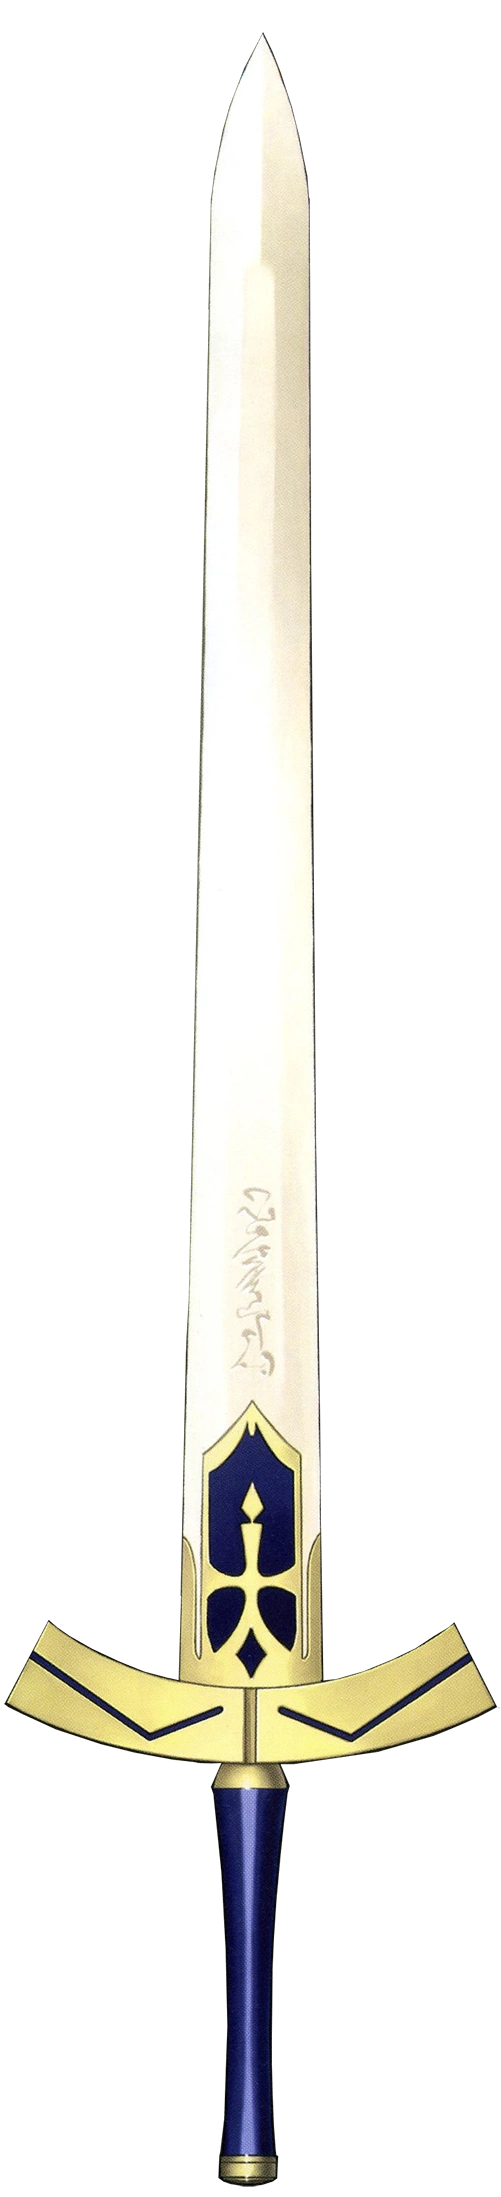
\includegraphics[width=0.15\textwidth]{Figs/Crests/Excalibur}}

%% College shield [optional] 
% Crest minimum should be 30mm.
%\collegeshield{\includegraphics[width=0.2\textwidth]{CollegeShields/Kings}}


%% Supervisor (optional)
%% for multiple supervisors, append each supervisor with the \newline command
%\supervisor{Prof. A.B. Supervisor\newline
%Prof. C.D. Supervisor}

%% Supervisor Role (optional) - Supervisor (default) or advisor
% \supervisorrole{\textbf{Supervisors: }}
%% if no title is desired:
% \supervisorrole{}

%% Supervisor line width: required to align supervisors
%\supervisorlinewidth{0.35\textwidth}

%% Advisor (optional)
%% for multiple advisors, append each advisor with the \newline command
%\advisor{Dr. A. Advisor\newline
%Dr. B. Advisor}
     
%% Advisor Role (optional) - Advisor (default) or leave empty
% \advisorrole{Advisors: }
%% if no title is required
% \advisorrole{}

%% Advisor line width: required to align supervisors
%\advisorlinewidth{0.25\textwidth}


%% You can redefine the submission text:
% Default as per the University guidelines:
% ``This dissertation is submitted for the degree of''
%\renewcommand{\submissiontext}{change the default text here if needed}

%% Full title of the Degree
\degreetitle{Doctor of Philosophy}

%% College affiliation (optional)
\college{Wolfson College}

%% Submission date
% Default is set as {\monthname[\the\month]\space\the\year}
%\degreedate{September 2014} 

%% Meta information
\subject{LaTeX} \keywords{{LaTeX} {PhD Thesis} {Physics} {University of
Cambridge}}


% ***************************** Abstract Separate ******************************
% To printout only the titlepage and the abstract with the PhD title and the
% author name for submission to the Student Registry, use the `abstract' option in
% the document class.

\ifdefineAbstract
 \pagestyle{empty}
 \includeonly{Declaration/declaration, Abstract/abstract}
\fi

% ***************************** Chapter Mode ***********************************
% The chapter mode allows user to only print particular chapters with references
% Title, Contents, Frontmatter are disabled by default
% Useful option to review a particular chapter or to send it to supervisior.
% To use choose `chapter' option in the document class

\ifdefineChapter
 \includeonly{Chapter3/chapter3}
\fi

% ******************************** Front Matter ********************************
\begin{document}

\frontmatter

\maketitle

%\begin{crests}

\hspace{25mm}

\includegraphics[width=0.20\textwidth]{Figs/Crests/Family_Crest}
\newline

\vspace{60mm}

\includegraphics[width=0.20\textwidth]{Figs/Crests/University_Crest.pdf}
\hspace{70mm}

\includegraphics[width=36mm, height=38mm]{Figs/Crests/Wolfson_Crest.png}

\end{crests}
% ******************************* Thesis Dedidcation ********************************

\begin{dedication} 

I would like to dedicate this thesis to my loving parents \dots

\end{dedication}
% ******************************* Thesis Declaration ***************************

\begin{declaration}

This dissertation is the result of my own work and includes nothing which is the outcome of work done in collaboration except as declared in the Preface and specified in the text. It is not substantially the same as any work that has already been submitted, or, is being concurrently submitted for a degree, diploma or other qualification at the University of Cambridge, or any other university or similar institution except as declared in the Preface and specified in the text. It does not exceed the prescribed word limit for the Faculty of Physics \& Chemistry Degree Committee.

\Cref{sec:21cm} reviews decades of research in 21-cm cosmology following the work of many authors cited throughout. \Cref{sec:edges} summarises the work done in relation to the experiments published as \citet{edgesNature} with \cref{sec:historic_cal} detailing the calibration methods used in the EDGES experiment introduced by \citet{rogersCal} and \citet{edgesCal}, though some equations have been changed in this thesis to conform with modern notation. \Cref{sec:receiver_general}, \cref{sec:additional_models} and \cref{sec:matlab_results} are intended to be published as \mbox{\citet{nimaCal}} which was initially co-written with Dr. Nima Razavi-Ghods. The work presented in this thesis has been rewritten and expanded to incorporate details not included in \citet{nimaCal}. Computer aided design (CAD) models for various devices developed for these experiments were created by Steven H. Carey and are credited as such in the image descriptions. Some of the CAD images and files have been altered by the author for presentation in this thesis. The experiment regarding the front-end thermal management system effectiveness on six litres of water was done independently by Steven H. Carey but is included here for completeness. \Cref{sec:reach_formalism}, \cref{sec:likelihood} and \cref{sec:simulated_data} have been published as \citet{ian_bayes}. \Cref{sec:mphil_results} summarises work submitted to the University of Cambridge for an MPhil degree entitled ‘Bayesian Techniques for the Calibration of 21 cm Global Experiments’. \Cref{sec:fbf} is work intended to be published by the author at a later date. \Cref{fig:amp1_schematic}, \cref{fig:amp2_schematic} and \cref{fig:fem_schematic} are circuit diagrams created by John A. Ely based on designs by Dr. Nima Razavi-Ghods.


\end{declaration}

% ************************** Thesis Acknowledgements **************************

\begin{acknowledgements}      

Firstly, my deepest appreciation (and sincerest apologies) go to my two supervisors; Dr. Nima Razavi-Ghods and Dr. Will Handley for their continued support, guidance and patience. I know I could not have been the easiest person to work with, and I am eternally grateful to have been taken on as a student by them.

Thanks to my dearest parents Thomas and Solon; I can’t believe how lucky I am to be their son. I wouldn’t trade it for the world.

Thanks to my loving family; Andrew, Ben, Dick, Lily, Matthew, May, Rachel, Solia and Susie, for waiting so patiently for me, and to my cherished grandmothers, Camila and Betty, for their everlasting love.

I truly could not have done this without my darling Sabrina. My heartfelt gratitude for putting up with me dear. A very special thanks to Waldemar and Martina for opening up their home to me, especially during the most critical and difficult periods of thesis writing. And thanks to Martha for the endless support and affection.

I am honoured by the fellowship and assistance of Dr. William Barker. Appreciation goes to Dr. Florian Lienhard for being the best office mate anyone could ask for, and to Prof. Dave Green for being the best office neighbour anyone could ask for. I also wish to acknowledge Steve Carey and John Ely whose hard work and knowledge were integral to this project, for which I am truly grateful. I am very grateful to my group as well. Dr. Dominic Anstey generously provided much of his time and expertise teaching me the mathematical background of which this work is based. Dr. Harry Bevins provided an ideal to strive for. Dr. John Cumner listened to every single one of my rants and helped me pull through on my worst days. Thomas Gessey-Jones patiently and thoroughly answered all of my questions regardless of how trivial they were or how many times I walked into his office unannounced. Thanks goes to Sam Leeney for all the support and lunchtime chats. I also wish to thank Kilian Scheutwinkel for all of the advice and encouragement. It really meant a lot to me.

Thanks goes to Prof. Patrick Carrazana for believing in me, to Prof. Richard Saunders for his boundless wisdom and to Dr. Thomas Feggeler for the continued professional advice. I am truly grateful for the guidance of Dr. Christopher O’Grady, Dr. Monarin Uervirojnangkoorn and Prof. Stefano Profumo. I would not be here without them. For changing how I see the world, I would like to thank Prof. Richard Mitchell and for starting me on this journey, I would like to acknowledge Mr. Steve Ratto. Ms. Katherine (Katie) E. Ward showed me endless kindness for which I am honoured as well. I am indebted to so many wonderful teachers who taught, supported and encouraged me including; Prof. Steven Ritz, Prof. George Brown, Prof. Enrico Ramirez‑Ruiz, Dr. Adriane Steinacker, Mr. Arron Apperson, Mr. Nate Kundin, Mr. David Martin, Mr. Asif Rahman, Mr. Rich Serrao, and Mrs. Cristina Trujillo.

I am grateful to Dr. Anas Al Rawi, Prof. Paul Rimmer, Mr. Anthony Djedi and Mr. Steven Brereton for their pastoral and professional support and to all my treasured friends met along the way; Khalid Aleem, Morgan Dang, Joe Ferris, Khalen Hudson, Perman Jorayev, Edii Lam, Liam Lau, James Luis, Derek Ngoon, Michael O'Donnghaile, Peter Pedersen, and Matt Wang. Franklin, Derek and Arun were the most genuine of friends even when I wasn’t, and I could not have done any of this without Will Mandell.

I give thanks to John and Michelle Bentley for their sincere kindness and belief in me. I would also like to acknowledge the colleagues we’ve lost; Prof. Richard Hills and Dr. David Sun who challenge us to be the best of scientists and of course, my beloved auntie Solane.

And finally, thanks goes to those who inspired me to undertake this endeavour in the first place; Dr. Neil deGrasse Tyson, Prof. Brian Greene, Prof. Brian Cox and Prof. Michio Kaku.

\end{acknowledgements}

% ************************** Thesis Abstract *****************************
% Use `abstract' as an option in the document class to print only the titlepage and the abstract.
\begin{abstract}
The detection of minute radio-frequency signals from the primordial Universe are thought to contain fundamental information on the evolution of the first luminous sources. Such breakthroughs however are hindered by the unprecedented levels of sensitivity and calibration needed to confidently distinguish these millikelvin-level signatures from galactic foregrounds and instrument systematics. In this work we detail the development of a calibration methodology that expands upon the Dicke switching procedure introduced for microwave-frequency devices and applies it to contemporary experiments targeting early time periods such as the Dark Ages, Cosmic Dawn and Epoch of Reionisation.

Included are the designs and practical considerations for a receiver unit housing numerous calibration standards, a compact microcontroller unit, portable vector network analyser and Peltier-based thermal management system for deployment with the REACH radiometer experiment in the South African Radio Astronomy Observatory. Following this, we detail a first-of-its-kind Bayesian calibration algorithm named \textsc{Excalibrate} which offers unparalleled speed and mobility, allowing for the characterisation of the radiometer in the same environment as observational measurements. Datasets taken at various points of the receiver development are tested with \textsc{Excalibrate} which archives calibration accuracies of about 1 kelvin or less.

Upon numerous adjustments to both the physical receiver unit and our code, we demonstrate that the polynomial approximation for calibration parameters used by \textsc{Excalibrate} may not be an appropriate model for continued advancement towards a tens-of-millikelvin-level calibration accuracy. We believe this finding is corroborated by the EDGES team, which calls into question the controversal results reported by them using similar polynomial approximations. In light of this, we derive a mathematical framework for an alternative method to solve for calibration parameters as singular values at each frequency point and conclude with further suggestions for increasing the sensitivity of the radiometer.

\end{abstract}


% *********************** Adding TOC and List of Figures ***********************

\tableofcontents

%\listoffigures

%\listoftables

% \printnomenclature[space] space can be set as 2em between symbol and description
%\printnomenclature[3em]

%\printnomenclature

% ******************************** Main Matter *********************************
\mainmatter

\pagenumbering{arabic}

\chapter{Introduction}

\ifpdf
    \graphicspath{{introduction/figs/Raster/}{introduction/figs/PDF/}{introduction/figs/}}
\else
    \graphicspath{{introduction/figs/Vector/}{introduction/figs/}}
\fi


%\section[Short title]{Reasonably long section title}
Only a year after its invention in 1608, the optical device known as the telescope was first pointed to the sky \citep{histTel}. In the four hundred years since, the tool has not only been the driver of astronomical research but epitomises the field and its achievements. Aided by the finite speed of light, our place in the Universe is contextualised through glimpses into the past, revealing galaxies up to eight billion years old in the visible spectrum. As we approach the limits of optical telescopes, novel methods of astrophysical observation are needed for continued advancements in our understanding of the cosmos. One such method is the employment of an instrument used to study information encapsulated in electromagnetic waves beyond the visible regime; the radio telescope \citep{smithObsAst}.

Over the past century, astronomers have pieced together the chronology of the Universe with studies such as the JWST Advanced Deep Extragalactic Survey which has unveiled galaxies nearly 13 billion years old \citep{jades}. Continued measurements reveal more information and even older structures using data at longer wavelengths such as the infrared \citep{abyss} as the wavelength of light from the oldest structures stretches with the expansion of the universe. This phenomenon is known as ‘redshift’ and relates the wavelength of an observed signal to its original wavelength when emitted in the distant past
\begin{equation}
    \label{eqn:redshift}
    1 + z = \frac{ \lambda_{\mathrm{obsv}} }{ \lambda_{\mathrm{emit}} },
\end{equation}
where $z$ is the dimensionless redshift quantity while $\lambda_{\mathrm{obsv}}$ and $\lambda_{\mathrm{emit}}$ represent the signal's wavelength at the time of observation and creation respectively. Redshift can be related to the extent of universal expansion to show the ages of objects in the sky and it can be shown that information from the earliest stars and galaxies have redshifted out the regime of visible light and into lower wavelengths. Thus, probing the deepest cosmic questions such as the development of galaxies within the first billion years of our Universe requires the use of low-frequency techniques \cite{furPhys}.

Since the 1930’s, radio telescopes have remained one of the most exciting research areas in contemporary astronomy with their potential to explore the first hundreds of millions of years after the Big Bang through observation of redshifted signals. By the 1950’s it was understood that, being the most abundant material in the Universe, study of hydrogen and its interaction with astrophysical phenomena would trace the bulk evolution of the cosmos as a whole, especially during periods where there is no visible light to be seen such as before the first stars. While the ultimate goal of current experimentation would be to analyse images of primordial hydrogen \citep{liuData,21in21}, the limitations of current technology restrict us to an interim objective of spectral measurements from the early universe. An essential tool for astronomers hoping to examine this time period would be to take advantage of hydrogen’s preference for specific wavelengths of light (particularly those with a wavelength of 21 centimetres), which manifest as minute changes in temperature profiles where energy is absorbed or released by hydrogen.


% =========================================
\section{21-cm astrophysics}\label{sec:21cm}
Following recombination, remnant photons from the Big Bang pervaded the Universe having escaped the frenzied soup of electrons now confined into neutral hydrogen atoms held together in gaseous form \citep{ryden}. In the present day, the expansion of the Universe has stretched the wavelengths of these relic photons out of the visible spectrum and into microwave frequencies which have been measured as the cosmic microwave background (CMB)\footnote{In this text, the relic photon field and the CMB will be referred to interchangeably.}. These hydrogen atoms interact restrictively with the CMB via photons of wavelength equal to 21 centimetres \citep{lofar}. Hydrogen atoms absorb these 21-cm photons and gain their energy causing the orientation of ground state electrons to flip relative to their associated nuclei \citep{furProbe}. This marginally higher-energy hydrogen atom is said to be in an ‘excited’ state compared to its natural orientation. 

Initially, the transfer of electrons between the neutral hydrogen gas and the CMB was in equilibrium preserving the CMB spectra predicted by the Planck formula at radio frequencies. During this time, the orientation of electrons in hydrogen atoms, also referred to as the spin state, were continuously swapped in equal proportion. For every 21-cm photon absorbed by the CMB, another was emitted by some nearby hydrogen atom as it decays from an excited state. Soon afterwards but before the existence of the first stars, hydrogen atoms in dense pockets collide to temporarily form hydrogen molecules in a process known as collisional coupling \citep{21in21}. The combination of two atoms mixes the orientation of the constituent electrons which, through the Universe’s natural preference for low-energy states, leads to a net de-excitation of electrons when the pairs dissociate. This sweeping reset of electron orientations down to their lowest energy configuration breaks the equilibrium state as more de-excited hydrogen atoms are free to absorb 21-cm photons from the CMB. This loss of 21-cm photons by the CMB should be seen as minute deviations from the spectrum predicted by the Planck equation allowing us to timestamp the construction of dense hydrogen pockets that would eventually coalesce into the first stars. This collisional coupling is only temporary though, as the expansion of the universe cools hydrogen adiabatically returning the primordial gas to equilibrium with the CMB as shown in \cref{fig:reionisation_hist} \citep{21in21}. This collection of processes in the absence of luminous sources is referred to as the Dark Ages.
\begin{figure}
    \centering
    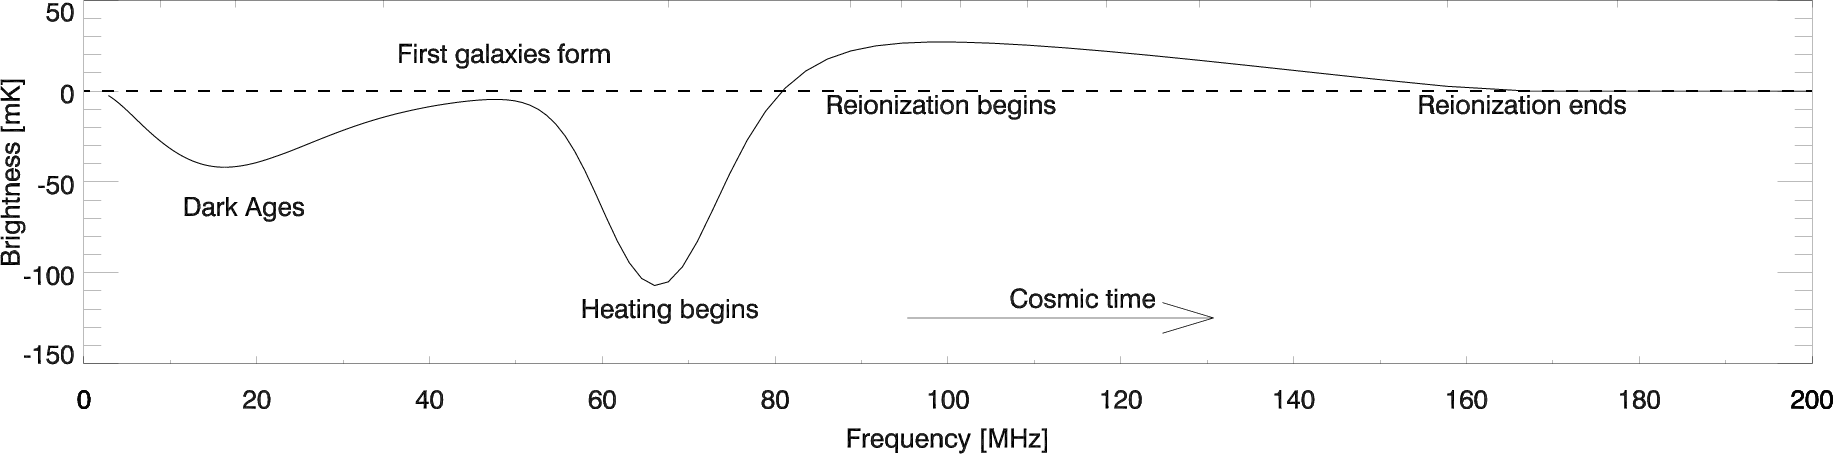
\includegraphics[width=\textwidth]{21cm_signal}
    \caption{A simulation of the expected 21-cm hydrogen signature based on typical models as a measurable brightness temperature (solid line) relative to the CMB temperature (dashed line). The turning points made from crests and troughs detail various stages of cosmic evolution such as the Dark Ages, the arrival of the first stars and galaxies, maturation of luminous sources and the Epoch of Reionisation. Image taken from \citet{cosmic_signature}.}
    \label{fig:reionisation_hist}
\end{figure}

The hydrogen gas in the most dense pockets eventually condenses into the first stars during Cosmic Dawn where ultraviolet (UV) radiation is generated for the first time since the Big Bang. Within this band of UV radiation are photons with a frequency of 2470 GHz known as a Lyman-$\alpha$ photon. These Lyman-$\alpha$ photons will bring the neutral hydrogen atoms to an energetic state beyond the spin flip which promptly decay down to the de-excited ground state, effectively cooling the gas and allowing for more absorption of CMB photons. This process, called the Wouthuysen-Field Effect, should yield an even stronger absorption trough than the collisional coupling as seen in \cref{fig:reionisation_hist} \citep{wouthuysen,field}. This first generation of stars will eventually mature into the first black holes and neutron stars producing even stronger radiation such as X-rays and gamma rays which will saturate the hydrogen gas and ionise them during an Epoch of Reionisation \citep{liuData}. The inability of hydrogen gas to continue absorbing photons will heat the gas past the CMB temperature leading to an emission profile as seen in \cref{fig:reionisation_hist}.

It is evident that CMB absorption and emission by primordial hydrogen gas traces early astrophysical processes that remain unconstrained by observation. Theory suggests that this may be measured as a differential brightness temperature relative to the predicted CMB profile and redshifted to radio frequencies between 50 and 200 MHz which can be represented by the equation
\begin{equation}
    \label{diffBright}
    \T{21} (z) \approx 0.023 \mathrm{K} \times x_{ \mathrm{H}_{\mathrm{I}} }(z) \left[ \left( \frac{0.15}{ \Omega_{\mathrm{m}} } \right) \left( \frac{ 1+z }{10} \right) \right]^{ \half } \left( \frac{ \Omega_{ \mathrm{b}} h}{0.02} \right) \left[ 1 - \frac{ \T{R}(z) }{ \T{S}(z) } \right],
\end{equation}
and is dependent on many characteristics of the early universe such as the fraction of hydrogen gas that is neutral $x_{ \mathrm{H}_{\mathrm{I}} }(z)$, the matter and baryon densities with respect to the critical density of the Universe $\Omega_\mathrm{m}$ and $\Omega_\mathrm{b}$ as well as Hubble’s constant $h$ \citep{edgesNature}. Also present in the equation is the temperature of the background radiation $\T{R}$ and the spin temperature $\T{S}$ which represents the relative populations of excited and de-excited electrons\footnote{The factor of 0.023 K comes from atomic-line physics \citep{edgesNature}}. Qualities of early luminous sources such as the efficiency of star formation or the mean free path of ionising photons will affect heating and alter the profile of the differential brightness temperature, producing a unique 21-cm brightness temperature such as the models shown in \cref{fig:21cm_models} where each individual line corresponds to a possible cosmic history \citep{theory_models}. Working backwards from an observed signal would provide constraints to these parameters narrating the influence of the first structures on the primordial hydrogen.
\begin{figure}
    \centering
    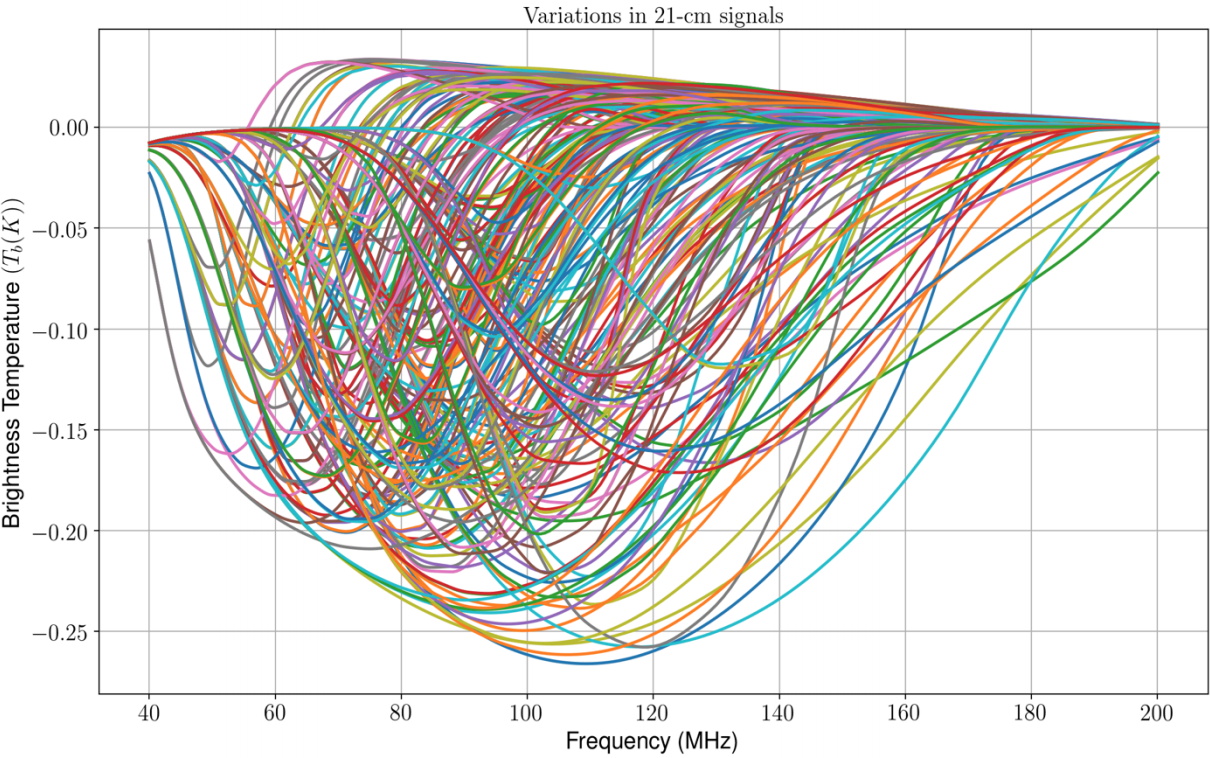
\includegraphics[width=0.8\textwidth]{21cm_models}
    \caption{Numerous simulations of plausible hydrogen signatures each representing a possible cosmic history. Various parameters such as the precise arrival of the first stars and galaxies will alter the hydrogen signal which when compared will allow theoreticians to identify models most representative of our early Universe. Data for image taken from \citet{theory_models}.}
    \label{fig:21cm_models}
\end{figure}


With the potential to provide such a wealth of information, many experiments have attempted to measure the 21-cm signature by taking long time integrations of radio spectra as a function of frequency averaged over the entire sky, also known as a ‘global’ measurement. This method has been employed in projects such as the Broadband Instrument for Global Hydrogen Reionisation Signal (BIGHORNS) \citep{bighorns}, the Large-Aperture Experiment to Detect the Dark Ages (LEDA) \citep{leda}, the Shaped Antenna Measurement of the Background Radio Spectrum (SARAS) \citep{saras} and the Sonda Cosmol\'{o}gica de las Islas para la Detecci\'{o}n de Hidr\'{o}geno Neutro (SCI-HI) \citep{scihi}. Another method of observation is the utilisation of interferometric arrays to measure spatial fluctuations in the sky brightness temperatures on the scales of megaparsecs which would give details on individual luminous sources. This technique is used in experiments such as the Low-Frequency Array (LOFAR) \citep{lofar}, the Precision Array for Probing the Epoch of Reionization (PAPER) \citep{paper}, the Hydrogen Epoch of Reionization Array (HERA) \citep{hera} as well as the future Square Kilometre Array (SKA) \citep{ska}.

Despite the developments in radio astronomy, a definitive detection of the 21-cm signature is yet to be made due to the difficulties that arise from such a measurement. One hindrance to experimentation are astrophysical foregrounds that may be up to five orders of magnitude higher than the proposed hydrogen signal at radio frequencies. These foregrounds include radiation produced from cosmic ray electrons moving through magnetic fields in our galaxy known as galactic synchrotron radiation, or the emission of photons when electrons scatter of the presently-ionised hydrogen nuclei known as free-free emission \citep{foregrounds,edges}. Fortunately, it is thought that the various crests and troughs of the 21-cm signature, known as ‘turning points’, allow the hydrogen signal to be distinguishable from the foregrounds which are smooth at radio frequencies and approximated by simple power law equations \citep{edgesNature}. Another point of concern are TV and FM radio broadcasts which are emitted at the frequencies relevant to 21-cm experiments \citep{reach}. Earth’s atmosphere is also known to be refractive at radio frequencies causing any potential signal to wander around the sky as ionospheric patches roll past the telescope’s observational beam \citep{lofar}. In response to these challenges however, scientists have developed models and methods to mitigate the effects of such impedances enabling continued studies which have provided intriguing results.


% =========================================
\section{The EDGES experiment}\label{sec:edges}
To date, the most significant result in 21-cm experimentation has been made by the Experiment to Detect the Global EoR Signature (EDGES) which aims to detect the sky-averaged 21-cm brightness temperature from the EoR \citep{edgesCal}. The project has been conducting multiple observations from the Murchison Radio-astronomy Observatory in Western Australia since 2006 \citep{edgesCal} using multiple dipole-like antennas of metal panels mounted horizontally above a ground plane \citep{edgesNature}. Early measurements placed an upper limit on the relative brightness temperature of the redshifted 21-cm signal contribution to their recorded foreground-removed spectrum \citep{edges2008} as well as a lower limit to the duration of the reionisation epoch with $\delta z > 0.06$, the latter result effectively excluding rapid reionisation models \citep{edges2010}. Following the deployment of one high-band and two low-band instruments, EDGES reported the detection of a flattened absorption profile in the radio spectrum centred at 78 MHz with a width of 19 MHz and depth of 0.5 K which they suggest is the 21-cm hydrogen signature \citep{edgesNature}.

The finding was met with considerable discussion as the detected profile’s characteristics did not match theoretical models. The trough centering at 78 MHz (corresponding to a redshift $z \sim 18$) would require more efficient star and galaxy formation at high redshifts \citep{edges_star_formation} while its flattened Gaussian shape suggest a delayed start to X-ray heating after the formation of Lyman-alpha emitting stars, not consistent with models \citep{theory_models}. Most notably however, was the profile amplitude which is more than a factor of two greater than the largest predictions by \citet{theory_models} as shown in \cref{fig:edges_signal} which would indicate that either primordial gas was cooler than expected or that the background radiation temperature was hotter than expected \citep{edgesNature}. With both the radiation and gas temperatures constrained by the CMB and adiabatic cooling mechanisms, known astrophysical processes are unlikely to account for the observed discrepancy and new physics has been proposed to to rectify the inconsistency such as an IGM cooling channel facilitated by dark matter-baryon interactions \citep{edgesNature}. Other phenomena such as an excess radio background due to efficient black hole formation obscured by dense hydrogen halos have also been proposed \citep{ew_radio_background}.
\begin{figure}
    \centering
    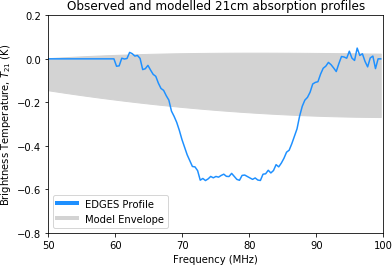
\includegraphics[width=0.7\textwidth]{edges_signal}
    \caption{The detected EDGES profile shown in blue \citep{edgesNature} over an envelope of models from \cref{fig:21cm_models} shown in grey. It is evident that the EDGES signal exhibits and absorption trough that is is deeper than all of the models shown. If astrophysical, this suggests and increased amount of CMB photon absorption by neutral hydrogen gas than previously expected. Additionally the flatness and width of the absorption trough are also unlike the models shown in \cref{fig:21cm_models}. All of these differences which may require new physics to explain. Data for EDGES signal available in footnote link \textsuperscript{c}. Data for model envelope from image by \citet{theory_models}.}
    \label{fig:edges_signal}
\end{figure}

Alternatively, inaccurate analysis methods or instrumental systematics may also account for the disparity between the EDGES data and theoretical models. \citet{hills_concerns} showed that the EDGES modelling process implied unphysical foreground emission parameters while \citet{sims_concerns} describe systematic calibration errors preferred by the Bayesian evidence under statistical analyses of the publicly available EDGES data\footnote{available at \url{http://loco.lab.asu.edu/edges/edges-data-release/}}. The \mbox{SARAS 3} radiometer measuring radio sky spectra at 55--85 MHz tested for the presence of the EDGES best-fit profile which was rejected from their data at the 95.3\% confidence level \citep{saras_reject}. Furthermore upper limits on the 21-cm power spectrum set by HERA Phase I observations were found to neither support nor disfavour a cosmological origin to the feature seen by EDGES \citep{hera_limits}.


The divided interpretation of the profile centred at 78 MHz highlights the need for follow-up experimentation to definitively confirm or refute the findings of \citet{edgesNature}. Continued investigations will need to improve on the instrumentation, analysis methods and measurement techniques in order to avoid data of nebulous origin or questionable interpretation. Many projects such as Probing Radio Intensity at high-Z from Marion (PRIZM) \citep{prizm}, Mapper of the IGM Spin Temperature (MIST) \citep{mist} and the Dark Ages Polarimeter PathfindER (DAPPER) \citep{dapper} are spearheading the effort including a certain Cambridge-led collaboration…


% =========================================
\section{The REACH experiment}\label{sec:reach}
The Radio Experiment for the Analysis of Cosmic Hydrogen (REACH) is a Cambridge-led sky-averaged 21-cm experiment of which the author is a member of. The radiometer targeting the cosmic hydrogen signature between 50--170 MHz ($z \sim $7.5--28) has a principle science objective of verifying the EDGES detection through a phased deployment at the RFI-quiet Karoo South African radio reserve \citep{reach}. A design focus on the identification and removal of residual systematics sets REACH apart from concurrent experiments which typically aim to minimise the chromatic response of the instrument as achromatic antennas mitigate the introduction of spectral components into foreground signals \citep{edges2008,saras2}. Relying on such a ‘smooth’ instrument response presents challenges such as with EDGES where the resulting frequency bandwidth ratio is restricted to 2:1 necessitating the use of scaled systems with overlapping bands to cover the full frequency range. REACH alternatively intends to improve on current experiments through the joint detection and characterisation of instrument systematics together with astrophysical foregrounds and the cosmic signature using Bayesian statistical methods \citep{dom,dom_modelling}. This joint fit between physically-based models is expected to facilitate the detection of correlated systematics and avoid those potentially degenerate with a cosmological signal with unaccounted-for systematics diagnosed using Maximally Smooth Functions \citep{maxsmooth}.

REACH Phase I plans on taking simultaneous observations of the sky using two antennas; the hexagonal dipole (50--130 MHz) and the conical log spiral (50--170 MHz) both of which were chosen from numerous designs for their ability to reconstruct mock 21-cm signals to a high degree of statistical confidence with small root mean square error in simulations \citep{dom_antenna}\footnote{We note that the hexagonal dipole is similar to the rectangular dipole antenna used in the EDGES experiment}. The antenna pair will be analysed in parallel to isolate signal components associated with hardware systematics while the contrasting mechanical designs will prevent experimental sensitivity to hardware-specific systematics. The project’s non-reliance on achromatic antennas allows for an ultra-wideband system covering the Cosmic Dawn and EoR (up to 3.5:1 for the conical log spiral) \citep{john_antenna}. Using such a large bandwidth, spectral differences between the oscillating 21-cm signature and the smooth power-law foregrounds can be leveraged during data analysis to support a positive detection \citep{reach}.

The deployment site was also chosen with care after an extensive survey. In the Karoo, REACH will observe the southern hemisphere sky from a remote 4 km wide basin surrounded by hills and mesas offering a reduced FM radio presence. Located near similar experiments such as HERA, MeerKAT \citep{meerkat} and the Square Kilometre Array (SKA)1-Mid instrument \citep{ska}, the location offers critical support infrastructure including on-site maintenance, staff as well as controlled access through paved roads. A Phase II experiment is planned for the same site which will incorporate additional antenna systems. Scaled versions of the hexagonal dipole and dual polarisation antennas have been proposed.

Simulations run with the above specifications forecast percent-level constraints on astrophysical parameters using REACH and in the case of a non-detection, upper limits on the strength of the absorption feature can be used to bound high-redshift phenomena \citep{reach}. We estimate a $\sim 500$ mK absorption profile consistent with EDGES can be detectable in as little as three hours of integrated data out of approximately 30 hours of observation time ($\lesssim \frac{1}{6}$th the time necessary to detect more conservative 21-cm signature models at the same redshift), though up to an order of magnitude more time may need to be allocated for the removal of low quality data and calibration measurements. If the data do not support an EDGES-like or high-amplitude 21-cm signal, the experiment will continue to integrate for longer periods in which case REACH will be able to place rigorous constraints on any excess radio background amplitudes and hydrogen cooling mechanisms beyond the typical adiabatic expansion. For the case of a detected 21-cm absorption signature much smaller than the EDGES profile in the high signal-to-noise regime, forward modelling consistent with standard astrophysics and cosmology will be used to constrain parameters such as the low-energy cutoff frequency and power law index of the X-ray spectral energy distribution, the X-ray efficiency of sources, the CMB Thomson-scattering optical depth, the minimum virial circular velocity of star-forming galaxies, the mean free path of ionising photons in the IGM as well as the star-formation efficiency \citep{tom_crh,visbal,fialkov_history}.

Contingent on this detection is of course, the measurement accuracy and sensitivity of the instrument as a whole. The contribution to this project by the author is the maximisation of such attributes through the construction of a high quality radio-frequency receiver unit, its seamless incorporation within the overarching system, as well as the development of intelligent software for receiver calibration. In this thesis, we present the designs, motivation, specifications and production of the REACH front-end and back-end receiver unit for deployment in 2023 highlighting its unique architecture and features to aid in instrument characterisation. We also detail an innovative calibration procedure that incorporates a Bayesian methodology leading to an in-field, rapid algorithm for calibration of the instrument in the same environment as observations, a first of its kind. While presenting the results of the technique, we highlight the challenges of achieving the accuracy needed to detect such miniscule 21-cm signals as well as present a framework for continued advancements in calibration towards the detection of the highly-redshifted global 21-cm hydrogen signature.


\chapter{Receiver design and development}\label{chap:instrumentation}

% **************************** Define Graphics Path **************************
\ifpdf
    \graphicspath{{instrumentation/figs/Raster/}{instrumentation/figs/PDF/}{instrumentation/figs/}}
\else
    \graphicspath{{instrumentation/figs/Vector/}{instrumentation/figs/}}
\fi

Measurements of the radio-sky require an instrument called a ‘radiometer’, a machine that measures incoming radiation. A radiometer usually consists of two main components; an antenna to collect electromagnetic waves and a device to measure the signal's power, such as a spectrometer. As more advanced instruments are deployed, additional processes are implemented to condition this information before being sent to the spectrometer such as amplification of weak signals and filtering to frequencies of interest such that a new intermediary device is often introduced as a bridge between the antenna and the spectrometer known as a ‘receiver’.

The addition of components such as a receiver will necessarily produce more complicated forms of systematic noise through things like reflections spawned from impedance mismatches at connections which hamper the detection and analysis of astrophysical phenomena. Characterising the interaction of the various instrument components as well as the resulting noise is undertaken through auxiliary devices which inform the process of ‘calibration’ in order to ultimately remove systematics and facilitate detection of cosmic signals. Consideration for the ensemble of devices, their control and monitoring is a principle area of experimental instrument design and the development of new architecture and engineering techniques to accommodate the unique requirements of individual experiments is the focus of this next chapter.


% =========================================
\section{The REACH receiver}\label{sec:receiver_general}
The REACH receiver is designed to address concerns brought forth from other experiments regarding residual systematics in their data while permitting the innovative features of the overall radiometer. Primarily, the broad bandwidth used by REACH makes it impractical to develop an achromatic antenna that provides a perfect impedance match between the antenna and receiver \citep{reach}. Reflections spawned from this contact point result in considerable spectral variation across the observational band on the order of tens of Kelvin due to the overwhelming synchrotron foreground at these frequencies. Furthermore, while the method of ‘relative calibration’ was historically used to characterise narrow-band instruments, wide-band radiometers must obtain an absolute flux scale in frequency to measure the frequency-dependent sky-averaged brightness temperature through ‘absolute calibration’ \citep{rogersCal}, which necessitates a series of additional components and switches.

Another primary focus of the design approach was the ability to calibrate the instrument completely in the field\footnote{While this philosophy was not completely adhered to in the final deployed system, the spirit of this ambition guided the entire receiver development. Please see \cref{sec:tparameters} for more details.} as opposed to previous experiments where the devices were characterised in controlled laboratory settings before deployment \citep{edgesCal}. The environmental (e.g. temperature and humidity) dependence of the sensitive electronic components provided a challenge to be addressed in the receiver design which requires system and temperature stability in the field as well as full autonomy.

In response to these considerations, the REACH receiver system is comprised of two subsystems, the receiver ‘front-end’ that sits under the raised antenna ground plane and the receiver ‘back-end’, also known as the readout system, which is separated from the front-end by a 100 metre distance connected by a Radio Frequency over Fibre (RFoF) link and powered by solar panels. A conceptual diagram of the radiometer system is shown in \cref{fig:system_diagram}. Many of the environment-sensitive components responsible for calibration and conditioning of the data are included in the front-end, with the back-end containing components for spectral data collection, control and signal processing as detailed below.
\begin{figure}
    \centering
    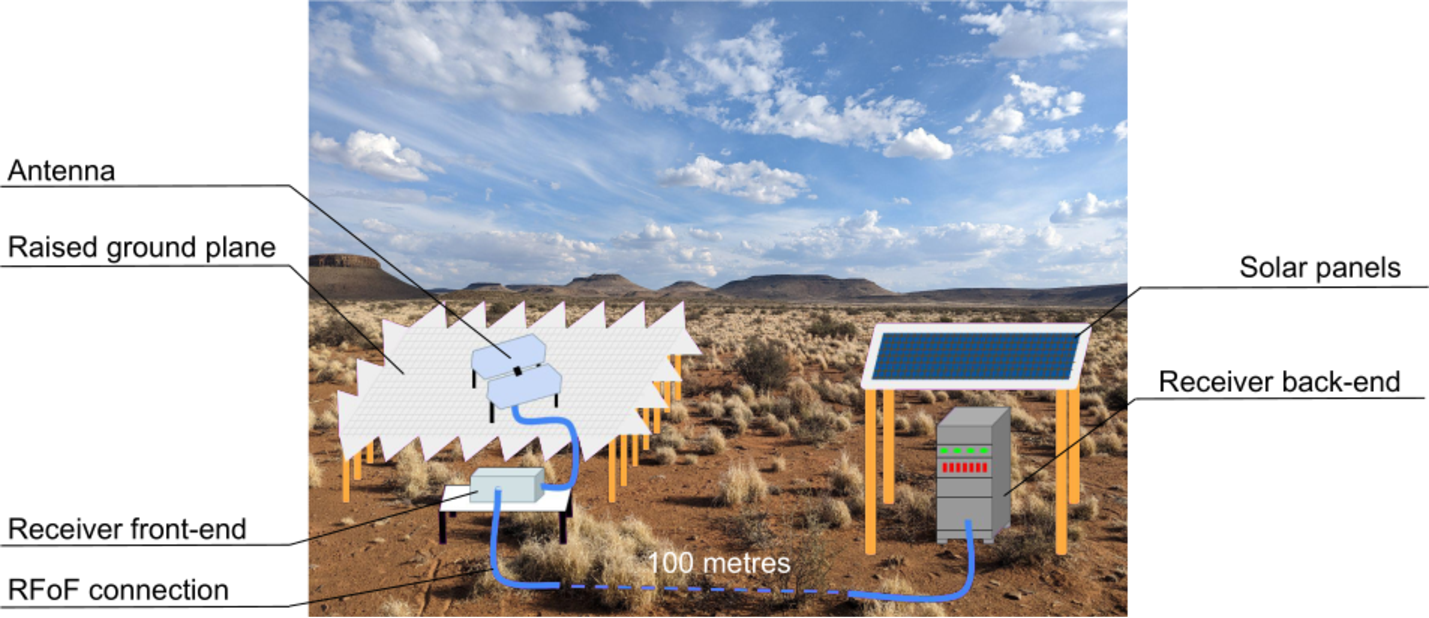
\includegraphics[width=\textwidth]{system_diagram}
    \caption{An illustration of the REACH radiometric system showing the hexagonal dipole antenna on a raised ground plane above the receiver front-end linked to the back-end and solar panels by 100 metres of fibre optic cable. The background image is a picture taken of the REACH deployment site located in the South African Karoo Radio Astronomy Reserve.}
    \label{fig:system_diagram}
\end{figure}


% =========================================
\section{Receiver front-end}\label{sec:frontend}
The front-end contains the most sensitive radiometer components housed in a sealed enclosure to facilitate calibration of the instrument to the highest accuracy. As the maintenance of environmental stability is difficult to achieve over long periods of time in the field, the project’s emphasis on an in situ calibration could only be achieved through a conscious effort to minimise the volume of the receiver front-end such that a constant temperature is kept via thermal devices while drawing a sustainable amount of power from the solar panels which allocate a maximum of 135 W of power to the front-end. Given this as a primary focus during the design process, nearly all of the components in the front-end were chosen based on a careful balance between their compact size and superior quality.


% =========================================
\subsubsection{The front-end enclosure}
The entirety of the receiver front-end is contained in a $500 \times 500 \times 210$ mm Rittal AE 1007.600 stainless steel enclosure serving as an RF-shield with category IP 66 protection against dust and water from the outside environment. 20 mm\footnote{18 mm in actuality when measured} of Kingspan Kooltherm K5 External Wall Insulation Board lines the inner walls of the enclosure in order to assist with temperature stability. Original designs used 11 mm Zotefoam for its efficient absorption of infrared radiation as used by the BICEP/Keck Array \citep{bicep}, but thermal tests showed this material to be less efficient during cooling compared to the 0.021 Wm\textsuperscript{-1}K\textsuperscript{-1} thermal conductivity of the building-standard Kooltherm sheets. Six connection ports were drilled into the enclosure to interface with external components; one for connection to the antenna sitting directly above the receiver on the raised ground plane via 150 mm Heliax cable, two for control and monitoring via USB over fibre-optical link, one RFoF connection for communication with the receiver back-end, one SubMiniature version-A (SMA) port for the 48 V DC power supply from the solar panels and an additional coaxial SMA port for testing and triage in the field. Electromagnetic interference (EMI) gaskets were placed around the openings to reduce the impact of self-generated RFI towards the antenna as well as external RFI from feeding into the signal chain. A diagram of the enclosure’s external connections is shown in \cref{fig:enclosure_external_connections}.
\begin{figure}
    \centering
    \includegraphics[width=\textwidth]{enclosure_external_connections}
    \caption{The external connections of the receiver front-end enclosure showing the coaxial antenna connections, USB to fibre connections in blue, RFoF connection in green, power connection and additional port for in-field diagnostics and testing. The orientation shown is the same as during deployment.}
\label{fig:enclosure_external_connections}
\end{figure}

The metal framing of the enclosure also served as a heat dump for the encased electrical components using a custom heat exchanger and fan-assisted heat sink as detailed in the next section. To assist with the thermal considerations, the receiver front-end components are mounted on a 3 mm baseplate as shown in \cref{fig:enclosure_plate} to allow airflow between the plate and the internal heat exchanger.
\begin{figure}
    \centering
    \begin{minipage}{.4\textwidth}
        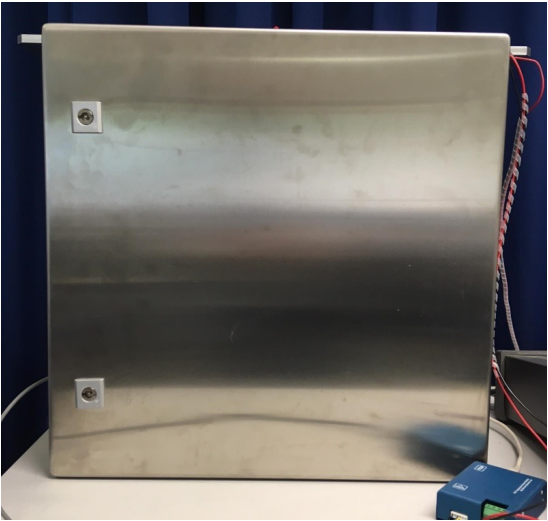
\includegraphics[scale=0.55]{enclosure}
        \vfill
        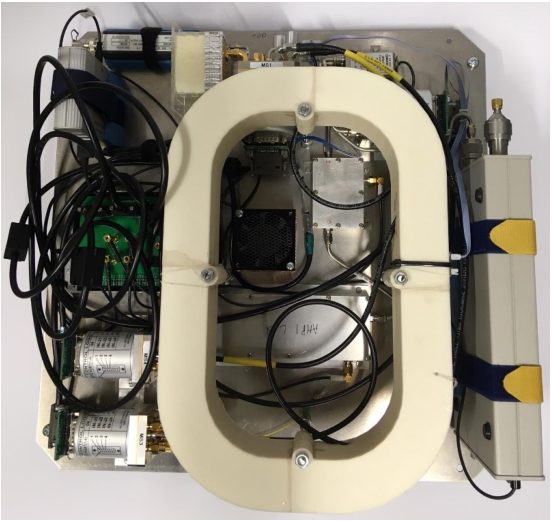
\includegraphics[scale=0.55]{component_plate}
    \end{minipage}
    \begin{minipage}{.4\textwidth}
        \centering
        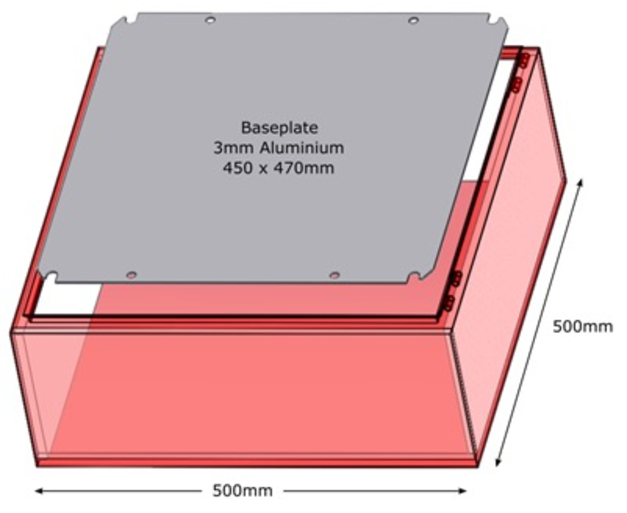
\includegraphics[scale=0.57]{enclosure_plate}
    \end{minipage}
    \caption{A picture of the front-end enclosure is shown on the top left. The bottom left shows the front-end components bolted onto the 3 mm baseplate. The diagram on the right depicts the baseplate's insertion into the enclosure. CAD image credit: Steven H. Carey.}
    \label{fig:enclosure_plate}
\end{figure}


% =========================================
\subsubsection{Front-end thermal management system}
Front-end temperature stability is maintained through a stack of components placed below the centre of the baseplate. A 113 watt Laird UltraTEC UT6-24-F1-5555 proportional integral derivative thermoelectric cooler (TEC) drives cooling or heating through the Peltier effect which is coupled to the receiver component baseplate by a $55 \times 55 \times 16$ mm copper stack. A thermal gap pad connects the bottom of the TEC module with a larger copper plate on the enclosure wall allowing heat transfer to an external Fischer LA7 150-1 heatsink and fan for expulsion of heat to the outside environment.

An initial test of this setup was conducted by placing a 40 W $110 \times 110$ mm heating source below the receiver component baseplate centre which recorded a 5 K temperature gradient over the plate as shown in \cref{fig:base_temp_grad}.
\begin{figure}
    \centering
    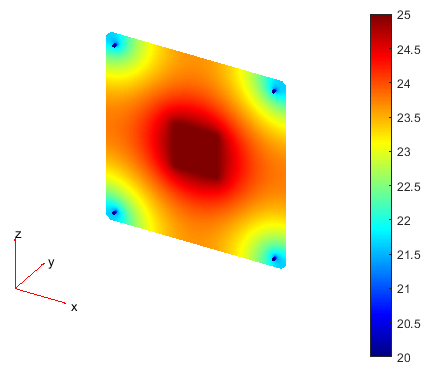
\includegraphics[scale=0.6]{base_temp_grad}
    \caption{A plot from an initial temperature test showing a 5 K temperature gradient over the receiver component baseplate when heated from below by a 40 W heat source placed at the plate's centre. Image credit: Steven H. Carey.}
    \label{fig:base_temp_grad}
\end{figure}
Following the results of this test, a secondary baseplate was installed below the initial baseplate with the two plates separated by a heatsink and an internal fan installed to promote air circulation throughout the front end. A follow-up test using this configuration returned a temperature gradient of 0.125 K across the component baseplate. A diagram of the completed setup is shown in \cref{fig:peltier_diag}
\begin{figure}
    \centering
    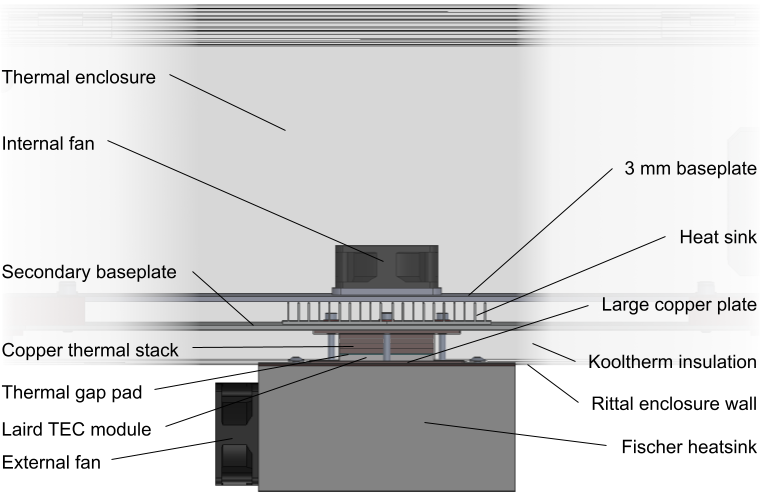
\includegraphics[width=\textwidth]{reach_peltier_diagram}
    \caption{A diagram representing the components for thermal conditioning of the receiver front-end. The vantage point shown is as if the front-end enclosure is laid on its back. It should be noted that the above figure is the MK II version which is slightly updated from the configuration currently deployed in the field. Modified from a CAD rendering by Steven H. Carey.}
    \label{fig:peltier_diag}
\end{figure}

The TEC is controlled by an Electron Dynamics Southampton TC-M-U-10A module and powered by a separate custom-made 22 V power supply unit (PSU) designed to reduce RFI coupling from the very large switch currents produced. The PSU, shown in \cref{fig:psu}, is also configured to automatically power the external fan when the Electron Dynamics controller draws more than 6 W of power to prevent thermal overload.
\begin{figure}
    \centering
    \begin{subfigure}{.45\textwidth}
        \centering
        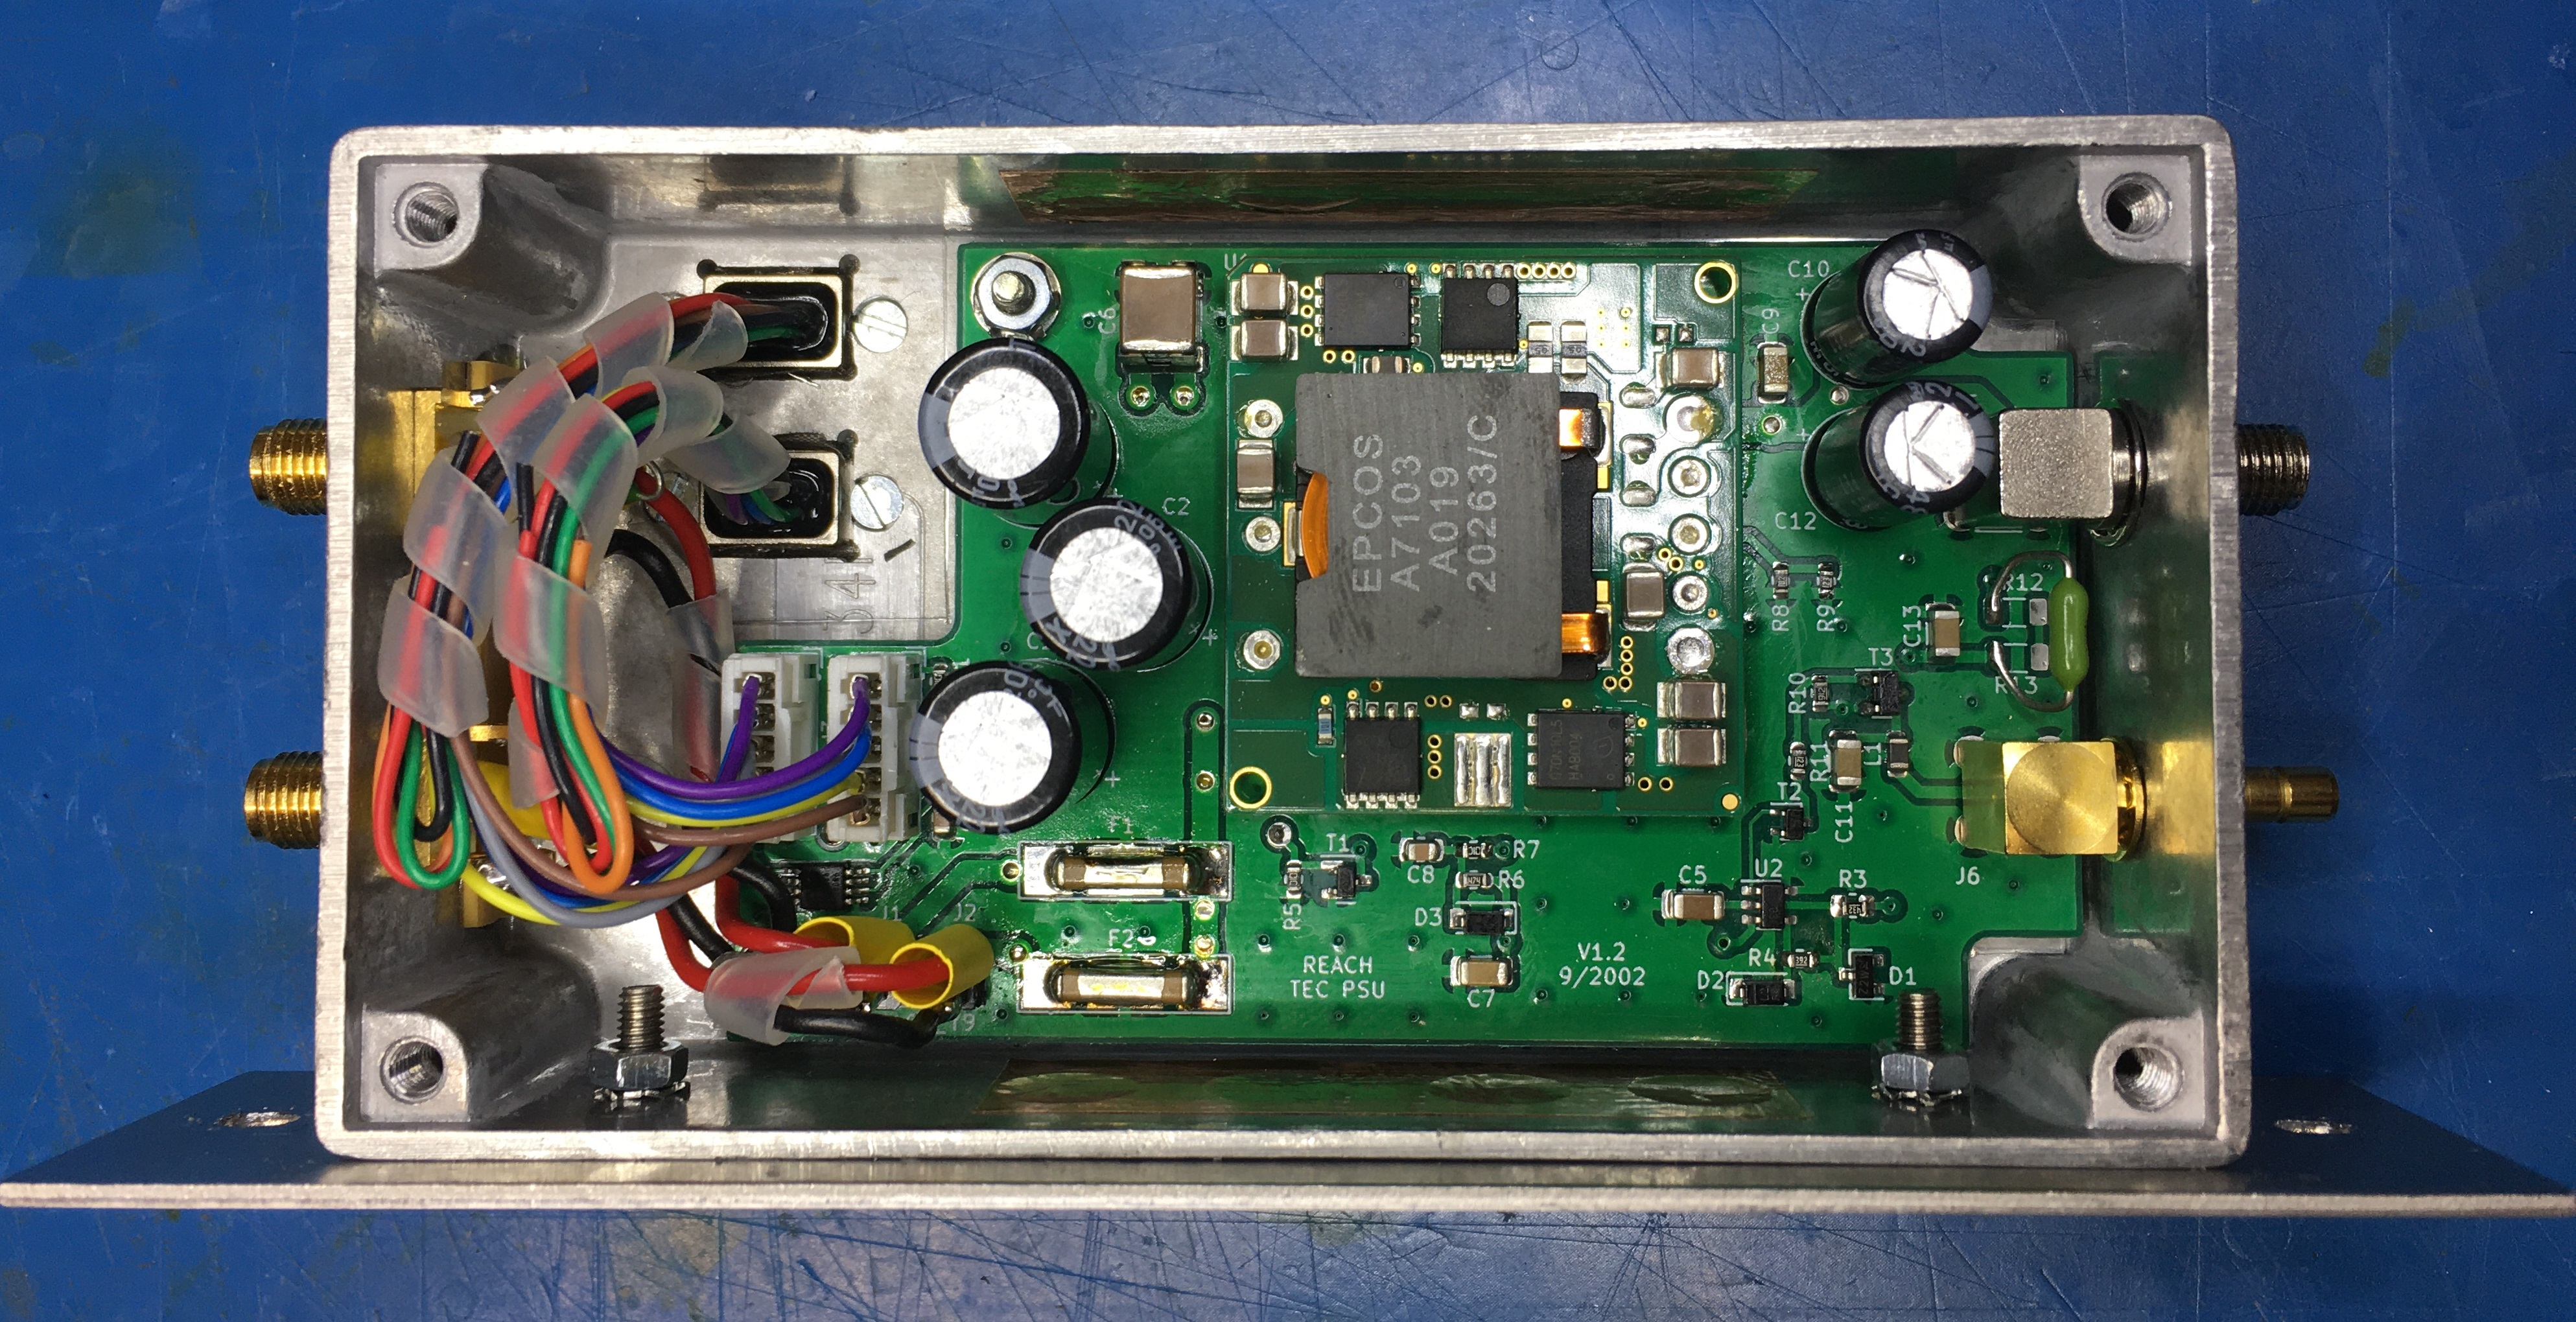
\includegraphics[width=\linewidth]{psu}
    \end{subfigure}
    \hfill
    \begin{subfigure}{.52\textwidth}
    \centering
        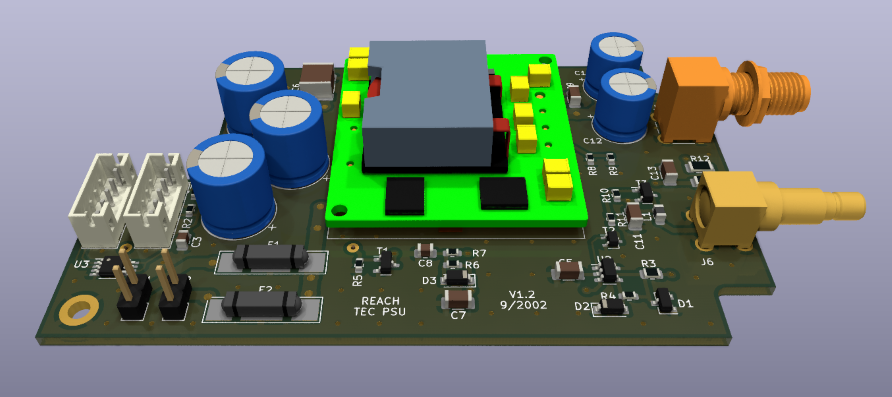
\includegraphics[width=\linewidth]{cad_psu}
    \end{subfigure}
    \caption{The constructed thermoelectric cooler power supply unit (left) along with its original CAD rendering (right) for perspective. CAD rendering credit: Steven H. Carey.}
    \label{fig:psu}
\end{figure}

The effectiveness of the front-end thermal management system was evaluated by testing the performance of the construction on 6 litres of bottled water placed in the empty front-end enclosure at room temperature with the TEC driven at its maximum 88 W and the Electron Dynamics controller instructed to maintain a $10^\circ$ C setpoint temperature as shown in \cref{fig:water_test} where the endpoint is achieved after about 8 hours of cooling with a steady-state temperature within 0.01 K of the target setpoint. These results suggest that a long, continuous amount of cooling is needed to stabilise the front-end temperature before calibration or observational measurements are made. This may be done in the afternoon or evenings preceding an observational run. An additional comparison of the completed thermal management system installed on the front-end enclosure with its 3D-rendered cross section is shown in \cref{fig:enclose_supp} for reference.
\begin{figure}
    \centering
    \centering
    \begin{subfigure}{.4\textwidth}
        \centering
        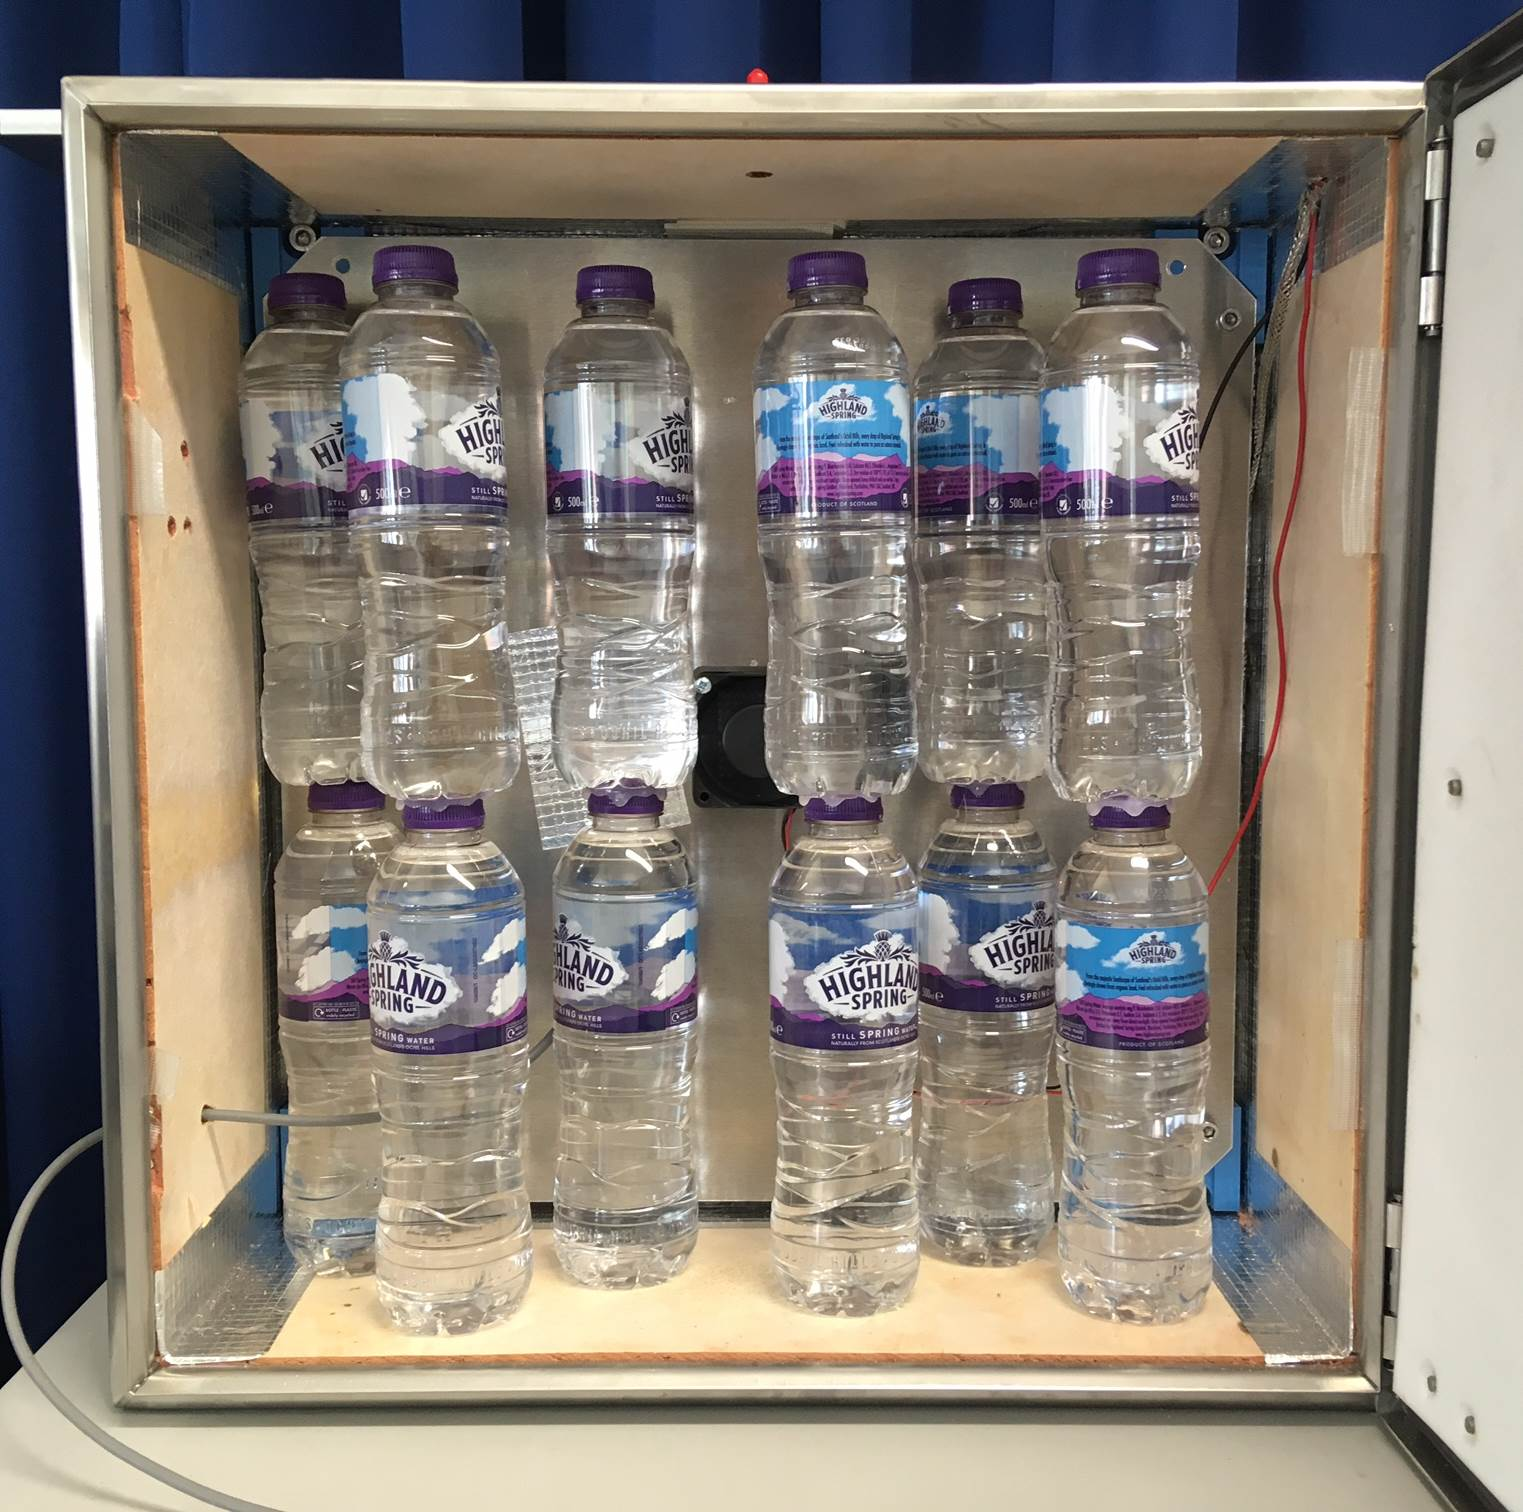
\includegraphics[width=\linewidth]{water}
    \end{subfigure}
    \hfill
    \begin{subfigure}{.55\textwidth}
    \centering
        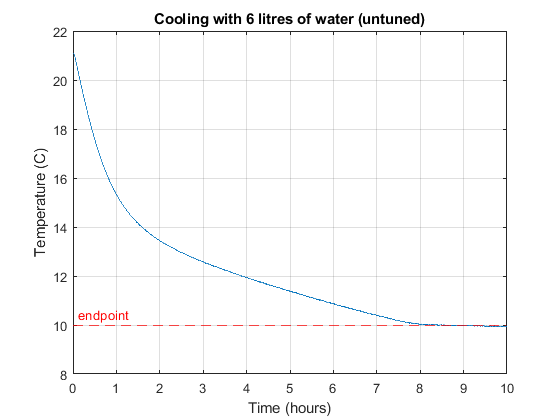
\includegraphics[width=\linewidth]{water_results}
    \end{subfigure}
    \caption{Six litres of water placed in the empty front-end enclosure with the thermal management system installed. The results of this test with the TEC driven at its maximum wattage and the controller setpoint of $10^\circ$ C is shown on the right. It should be noted that for this test, the proportional, integral and derivative controller values were not tuned beforehand, which reduces efficiency. Image credit: Steven H. Carey.}
    \label{fig:water_test}
\end{figure}


% =========================================
\subsubsection{Calibration sources}
One of the main obligations for thermal stability is to stabilise measurements of passive devices used to calibrate the instrument which we collectively refer to as ‘calibration sources’ or ‘calibrators’. Historically, absolute calibration is undertaken through measurement of each calibration source as part of a three-position Dicke cycle containing a single source, a reference $50 \Omega$ load and a reference noise source where comparison of power spectral measurements between the source and references serve to calibrate out time dependent system gain using \cref{eqn:tant_star} \citet{edgesCal,rogersCal}. Usually four sources were used; 1) an ambient-temperature ‘\textit{cold}’ $50 \Omega$ load, 2) a $50 \Omega$ load heated to high temperature, 3) a cable shorted at one end and 4) a cable left open at one end. The $50 \Omega$ loads give the absolute temperature scale in our calibration solution while the cables simulate antennas looking at an isotropic sky with temperatures equal to the cables’ physical temperature \citep{rogersCal}. A diagram of the Dicke switching procedure used in calibration is shown in \cref{fig:dicke}.
\begin{figure}
    \centering
    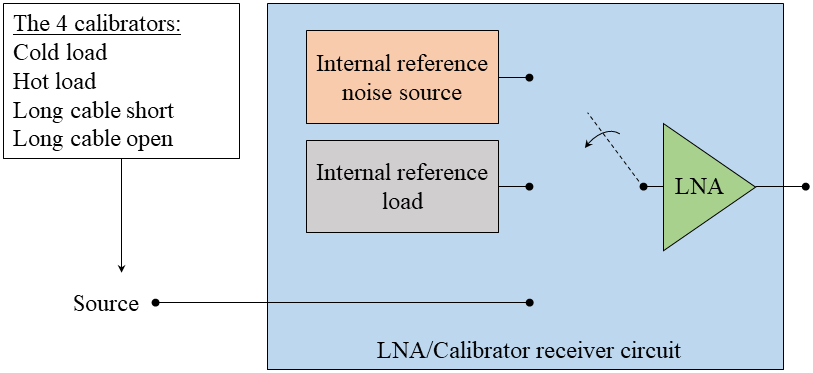
\includegraphics[scale=0.5]{dicke}
    \caption{A diagram of the Dicke switching procedure showing the calibrator position, $50 \Omega$ reference position and reference noise source position. Here, the four canonical calibration sources are used; the ambient and heated $50 \Omega$ loads along with the shorted and open cables. Power spectral measurements of these devices are conditioned by the Low Noise Amplifier (LNA) before being passed on to the spectrometer for initial removal of the time-dependant system gain.}
    \label{fig:dicke}
\end{figure}

The cold load used was taken from an 85033 $50 \Omega$ SMA calibration kit certified by Kirkby Microwave. Multiple heated loads were custom made for this experiment. A simple heated load was constructed from a 4-inch RG-405 coaxial cable terminated with a $50 \Omega$ load attached to a proportional heater connected to DC power with the temperature directly monitored through contact with a thermocouple. As the heated calibration source is typically heated to $\sim 370$ K, which could affect the temperatures of nearby ambient components, an improved calibrator was constructed with the $50 \Omega$ resistor and thermistor attached to a 4-inch semi rigid cable surrounded with thermal insulation and encased in an acrylic cubic shell. A temperature gradient across the 4-inch cable within the construction is produced by the temperature difference between the heated load and the coaxial end connected to the receiver input. As this changes the temperature ‘seen’ by the instrument, a corrective factor is introduced in our calibration calculations and detailed in \cref{sec:historic_cal}. While this advanced heated load was used for some of the results presented in this work such as in \cref{sec:hera_results} and \cref{sec:reach_results}, the simple heated load was the device deployed to the field due to time constraints impacting critical adjustments to reinforce the advanced heated load. A diagram of the advanced heated load is included in \cref{fig:hot_load}.
\begin{figure}
    \centering
    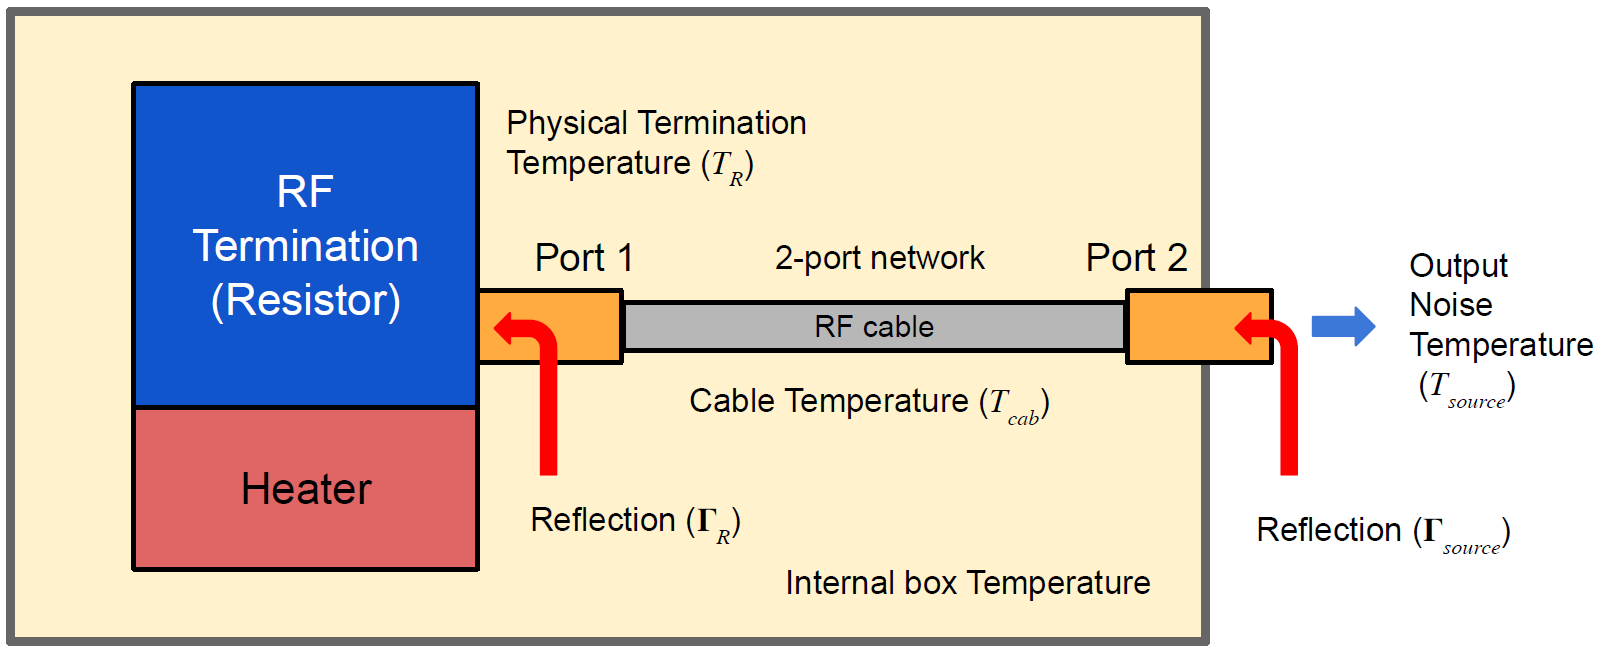
\includegraphics[width=0.65\textwidth]{hot_load}
    \caption{Illustration of the heated load construction for use as a calibration source. The thermally enclosed resistor and powered heater are connected to the input switch via a 4-inch cable as shown in the diagram. These components effectively form a temperature gradient across the calibration device which must be corrected for via the procedure discussed in \cref{sec:historic_cal} as $\T{R}$, $\T{cab}$ and $\T{source}$ are not necessarily equal.}
    \label{fig:hot_load}
\end{figure}

Open and shorted coaxial terminations were taken from the same Kirkby 85033 kit and connected to the end of coaxial cables. Over the course of receiver development, many different models and lengths of cables with varied specifications were tried with the final deployed system having the open and shorted ends connected to 10 metre LMC195 coaxial cabling partially built in-house at Cambridge. With the need for more accurate characterisation of the instrument, we have expanded our selection of calibration sources to twelve, maximising the information detailing the instrument response. Additional ambient-temperature $25 \Omega$ and $100 \Omega$ resistors were included for increased data on non-complex impedance response. The same 10 metre LMC195 cable was also terminated with $10 \Omega$ and $250 \Omega$ resistors. An additional 2 metres of LMC195 terminated with $27 \Omega$, $36 \Omega$, $69 \Omega$ and $91 \Omega$ resistors was also included. These additional terminations were all custom made in Cambridge.

The calibration sources and resistances were carefully chosen to permit strategic sampling of the noise waves as a function of impedance. \Cref{fig:smith} demonstrates the extensive scope of frequency-dependent impedances for our calibration sources as well as a simulated impedance of the REACH dipole antenna covering 50--150 MHz \citep{john_antenna}.
\begin{figure}
    \centering
    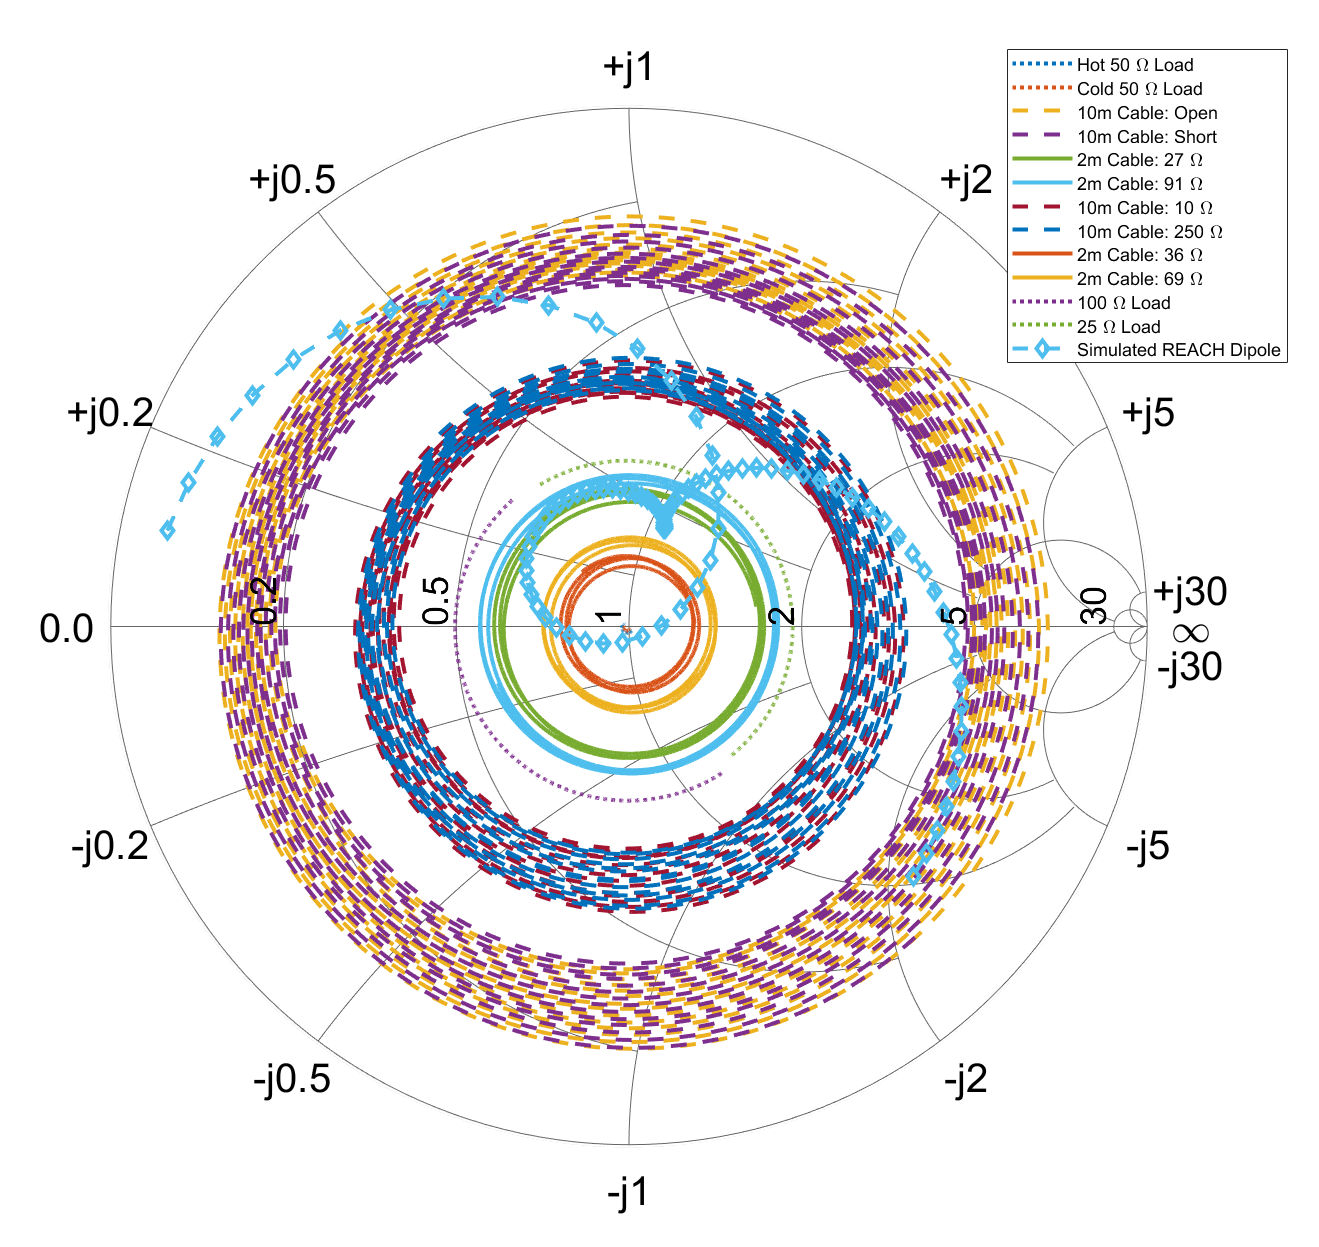
\includegraphics[scale=0.3]{smith}
    \caption{Smith Chart showing the impedance of twelve calibration sources and the simulated REACH antenna (internal variant \#0744) with the centre of the plot indicating an impedance of 50 $\Omega$. The plot ranges from 50--150 MHz with the antenna curve starting at 50 MHz on the left-hand side. The extensive coverage in impedance space by our calibration standards can be interpreted as a substantial amount of information regarding the characteristic response of the instrument. Note that the impedances of the ambient and heated 50 $\Omega$ loads lie directly in the middle of the chart and are partially obscured by the antenna plot. Updated from figure included in \citet{reach}}
    \label{fig:smith}
\end{figure}
\Cref{fig:smith} also demonstrates measurements of the $25 \Omega$ and $100 \Omega$ loads as half circles on the Smith chart, which differs from the theoretical points at $25 \Omega$ and $100 \Omega$ due to the practical limitations of real-world impedance measurement and exacerbated by the additional RF path in our receiver between the sources and the measurement reference plane for the reflection coefficients. These effects were the motivation for the corrections detailed in \cref{sec:tparameters}.

Power spectral measurements are taken of two reference sources for every measurement of a calibration source to divide out the short-time variability in receiver gain as previously stated. Ideally, the reference load would be a separate $50 \Omega$ load of high quality such as from an additional certified calibration kit, but due to time constraints in the deployment, a repeated measurement of the ambient load used as a calibration source was taken. As these Dicke switch measurements detail the changing gain of the system \citep{edgesCal} and not the absolute differences between the devices used as calibration sources and reference sources, we believe that this degeneracy would not severely impact the quality of the results presented in this work.

The reference noise source used is a Noisecom NC346A. An important distinction must be made here between the heated $50 \Omega$ load as a calibration noise source and the Noisecom noise diode used as a reference noise source. While the constant noise power provided by the noise diode is necessary for maximal radiometer measurement accuracy through removal of the time-dependent gain fluctuations via the Dicke switching procedure, the direct and accurate measurement of the heated $50 \Omega$ load via thermocouple is beneficial for the removal of systematic noise via accurate noise wave parameter derivation. 

Noise output data of the reference noise diode as provided in decibel excess noise ratio by Noisecom in shown in \cref{tab:ns_noise}.
\begin{table}
    \begin{center}
    \begin{tabular}{ |c|c| }
        \hline
        {Frequency} & {Excess noise ratio} \\
        \hline
        30 MHz & 6.05 dB \\
        40 MHz & 6.03 dB \\
        50 MHz & 6.00 dB \\
        60 MHz & 5.94 dB \\
        70 MHz & 5.91 dB \\
        80 MHz & 5.87 dB \\
        90 MHz & 5.84 dB \\
        100 MHz & 5.79 dB \\
        110 MHz & 5.80 dB \\
        \hline
    \end{tabular}
    \quad
    \begin{tabular}{ |c|c| }
        \hline
        {Frequency (contd.)} & {Excess noise ratio (contd.)} \\
        \hline
        110 MHz & 5.80 dB \\
        120 MHz & 5.77 dB \\
        130 MHz & 5.80 dB \\
        140 MHz & 5.81 dB \\
        150 MHz & 5.83 dB \\
        200 MHz & 5.88 dB \\
        250 MHz & 5.87 dB \\
        350 MHz & 5.87 dB \\
        500 MHz & 5.89 dB \\
        \hline
    \end{tabular}
    \end{center}
    \caption{Manufacturer quoted noise output for the Noisecom NC346A noise diode used as the reference noise source within the Dicke switching procedure as an excess noise ratio. The stability of the noise output within the REACH observational band (50--130 MHz) at these scales should be noted, which is beneficial for the removal of time-dependent system gain.}
    \label{tab:ns_noise}
\end{table}
We can convert the noise output values from \cref{tab:ns_noise} to linear scale using the equation
\begin{equation}
    \mathrm{ENR_{dB}} = 10 \cdot \log_{10} \left( \frac{T - 290}{290}\right),
\end{equation}
with 290 being the standard reference temperature for noise and $T$ as a linear-scale excess noise above ambient temperature (assumed to be 298 K). A plot of the linear noise output of the reference noise diode with ambient temperature subtracted is provided in \cref{fig:ns_diode} which may serve as a potential sanity check for our calibration algorithm as these values inform us of the approximate values of the $\T{NS}$ noise wave parameter as verified in \cref{fig:ls_nwps}. This value may not be exactly replicated however, due to the additional RF path introduced earlier and again detailed in \cref{sec:tparameters}. It should also be noted that these values are exclusive to this particular noise source and the use of different noise diodes in future builds, including identical model numbers, would necessarily be different and require recalculation following the above prescription.
\begin{figure}
    \centering
    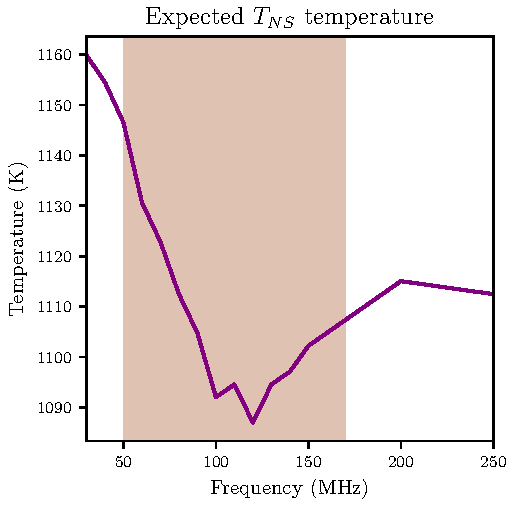
\includegraphics[width=0.5\textwidth]{ns_diode}
    \caption{A plot of the reference noise diode output from the datasheet provided by Noisecom with the REACH observational band (50--130 MHz) as the shaded region. The scale of the plot allows us to gauge the values expected of the $\T{NS}$ noise wave parameter from our calibration algorithm. As the variation shown in the diagram is about six percent over the frequencies of interest, we consider the noise diode stable at these temperature scales. It is considered impractical to attempt to heat a device such as a load to similar temperatures in the field and thus we rely on an effective noise temperature from the diode imitating the noise of a black body at $\sim$1100 K. As an effective noise temperature, measurement of the diode output via thermocouple as done with the calibration sources is not possible, necessitating alternative forms of verification such as comparison between the $\T{NS}$ parameter and the manufacturer datasheet.}
    \label{fig:ns_diode}
\end{figure}


% =========================================
\subsubsection{Switches}
The sizeable battery of calibration and reference sources may seem at first glance to run against the primary goal of having a small-volume receiver. To meet this challenge, a complicated network of mechanical switches was conceived to allow for the myriad components and various signal paths through the instrument. The essential calibration sources mentioned in the previous subsection were gathered on an 8-way switch (referred to as MS1) with switch positions one through six taken up by the antenna, cold load, reference noise source, heated load, $25 \Omega$ load and $100 \Omega$ load respectively. To avoid the size requirements of having multiple calibration cables with various terminations, a single 2 metre LMC195 cable and 10 metre LMC195 cable were connected to MS1 positions seven and eight with the opposing ends of the cables connected to their own 4-way switch referred to as MS3 and MS4 respectively. These cable switches were connected to the appropriate terminations according to the previous subsection; $36 \Omega$, $27 \Omega$, $69 \Omega$ and $91 \Omega$ for MS3 positions one through four as well as open termination, shorted termination, $10 \Omega$ and $250 \Omega$ for MS4 positions one through four for the 2 metre and 10 metre cables. A custom 3D-printed structure was designed to house the two calibration cables within the receiver front-end which is highlighted in \cref{fig:stadium}
\begin{figure}
    \centering
    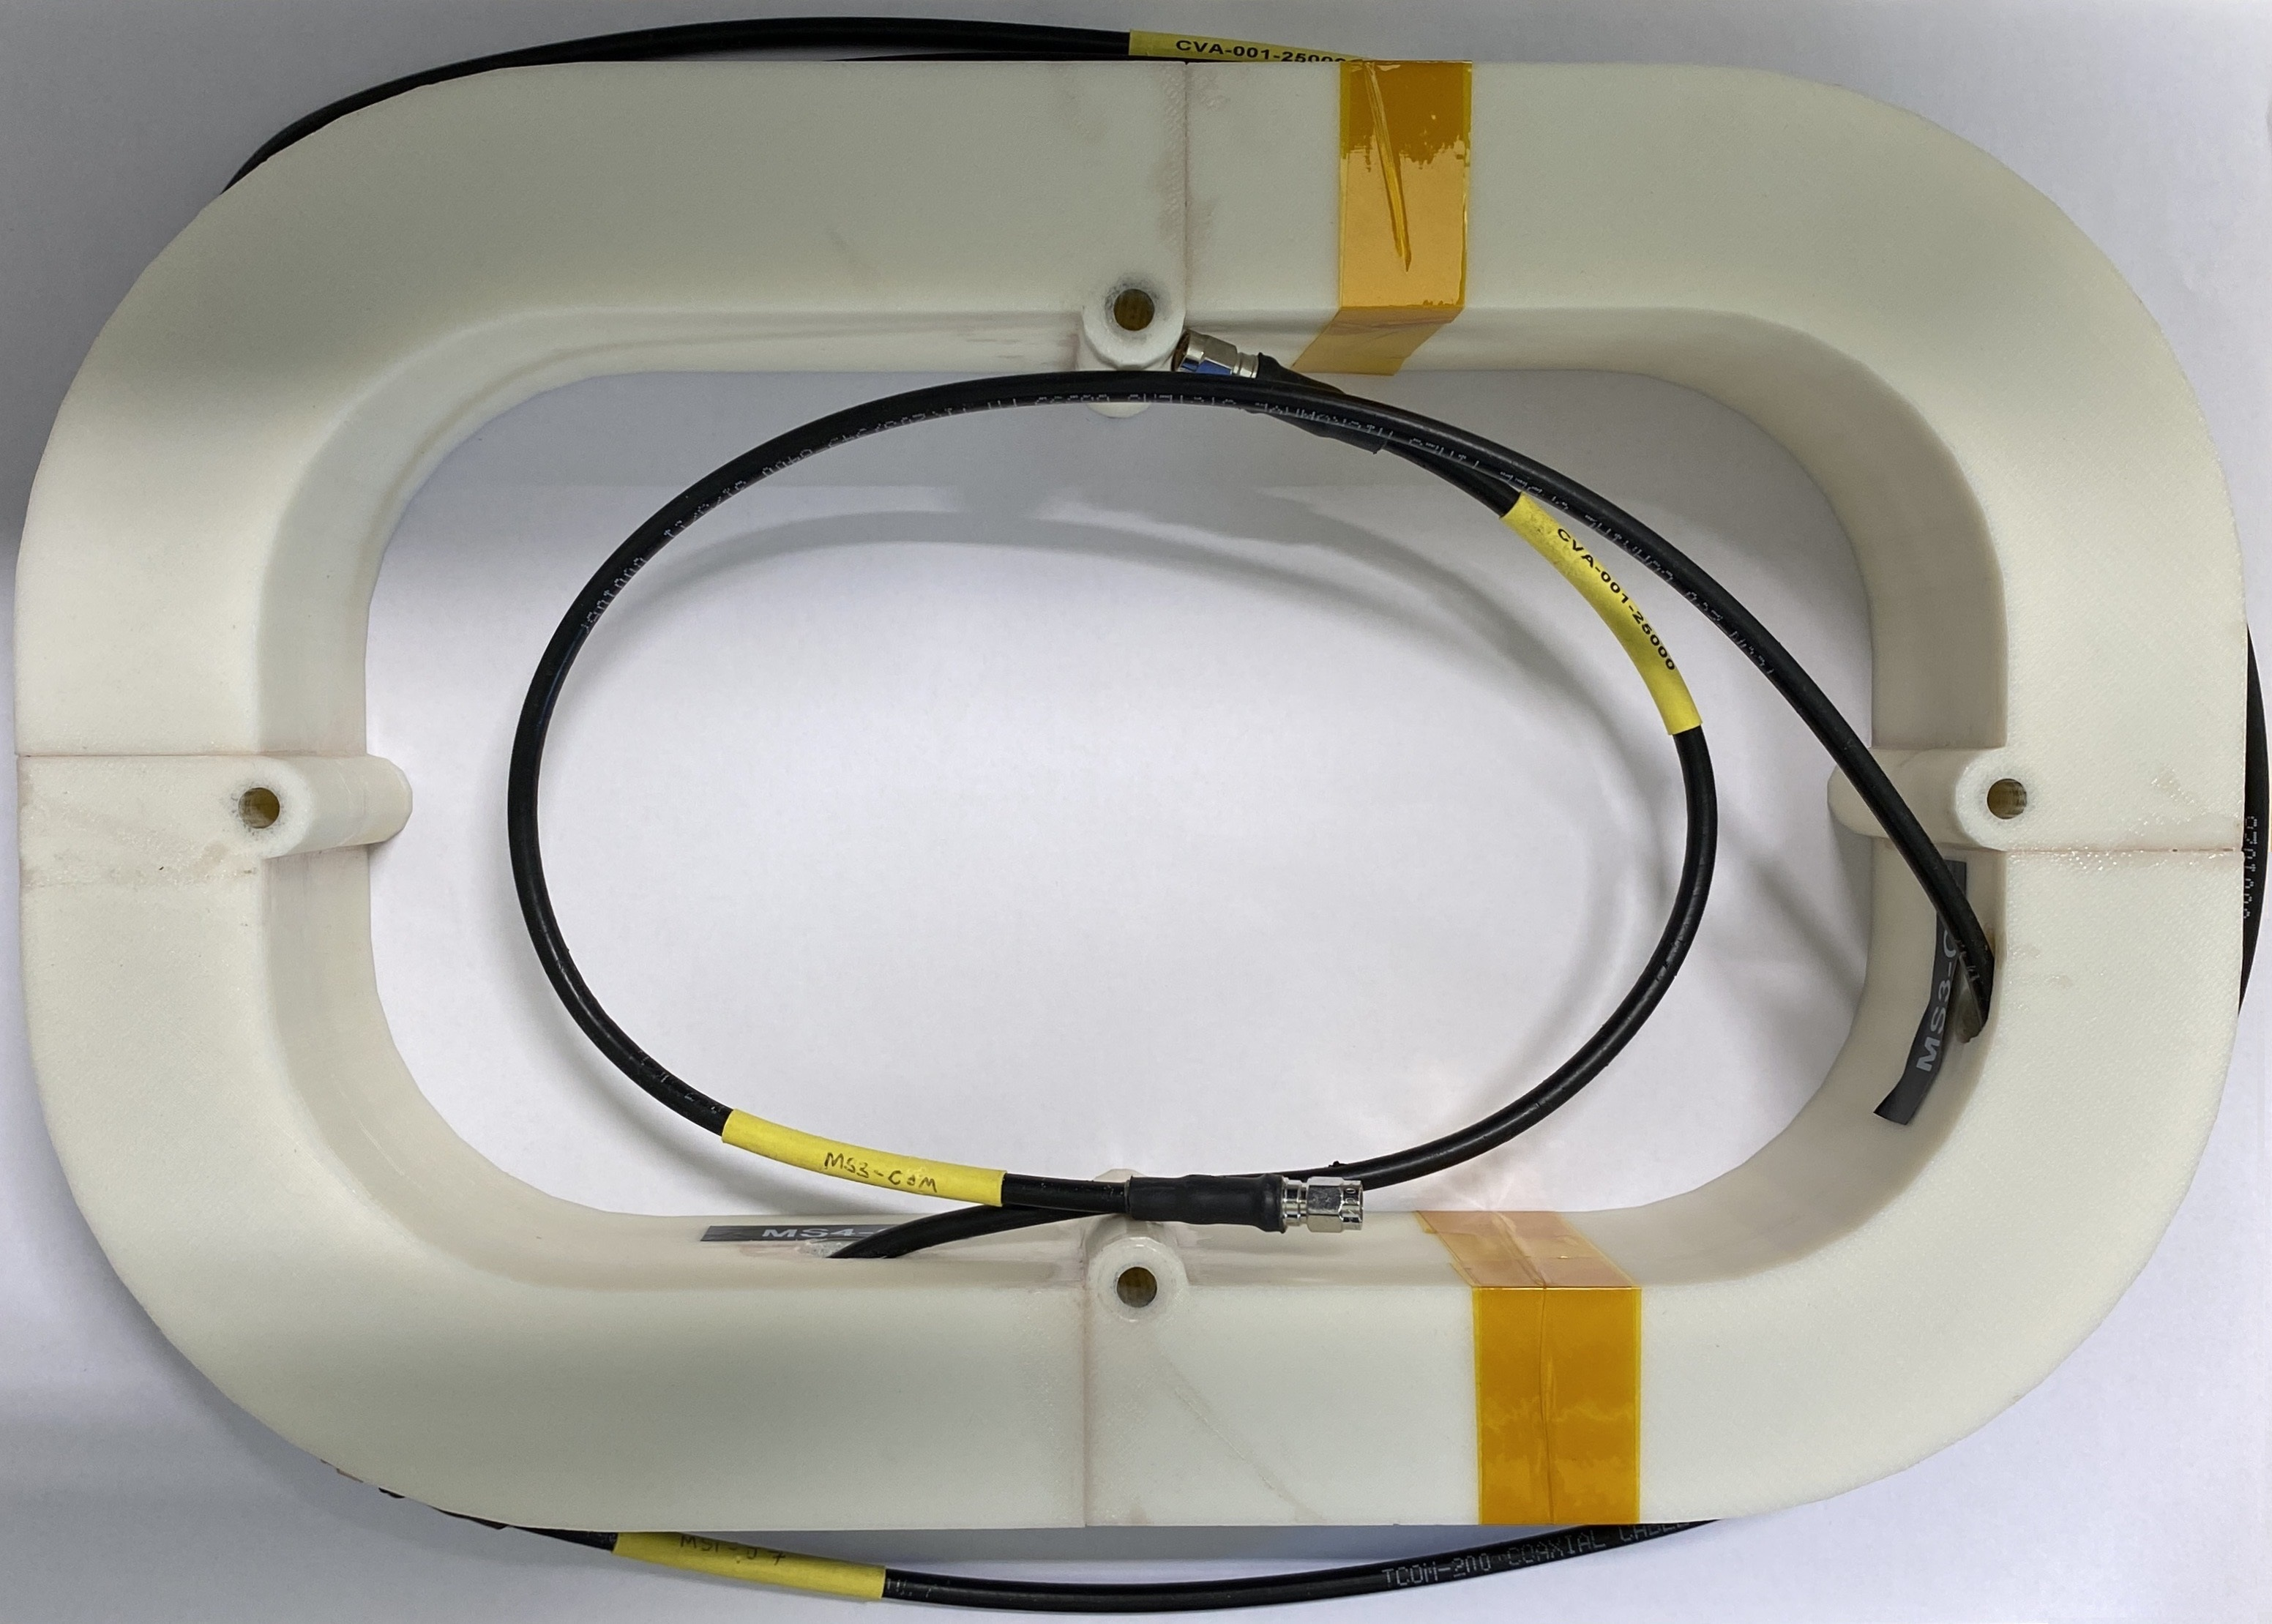
\includegraphics[width=0.65\textwidth]{stadium}
    \caption{3D printed housing for the 2 metre and 10 metre calibration cables. This unit is affectionately referred to as ‘the stadium’.}
    \label{fig:stadium}
\end{figure}

A schematic block diagram of the switching configuration is shown in \cref{fig:overview}.
\begin{figure}
    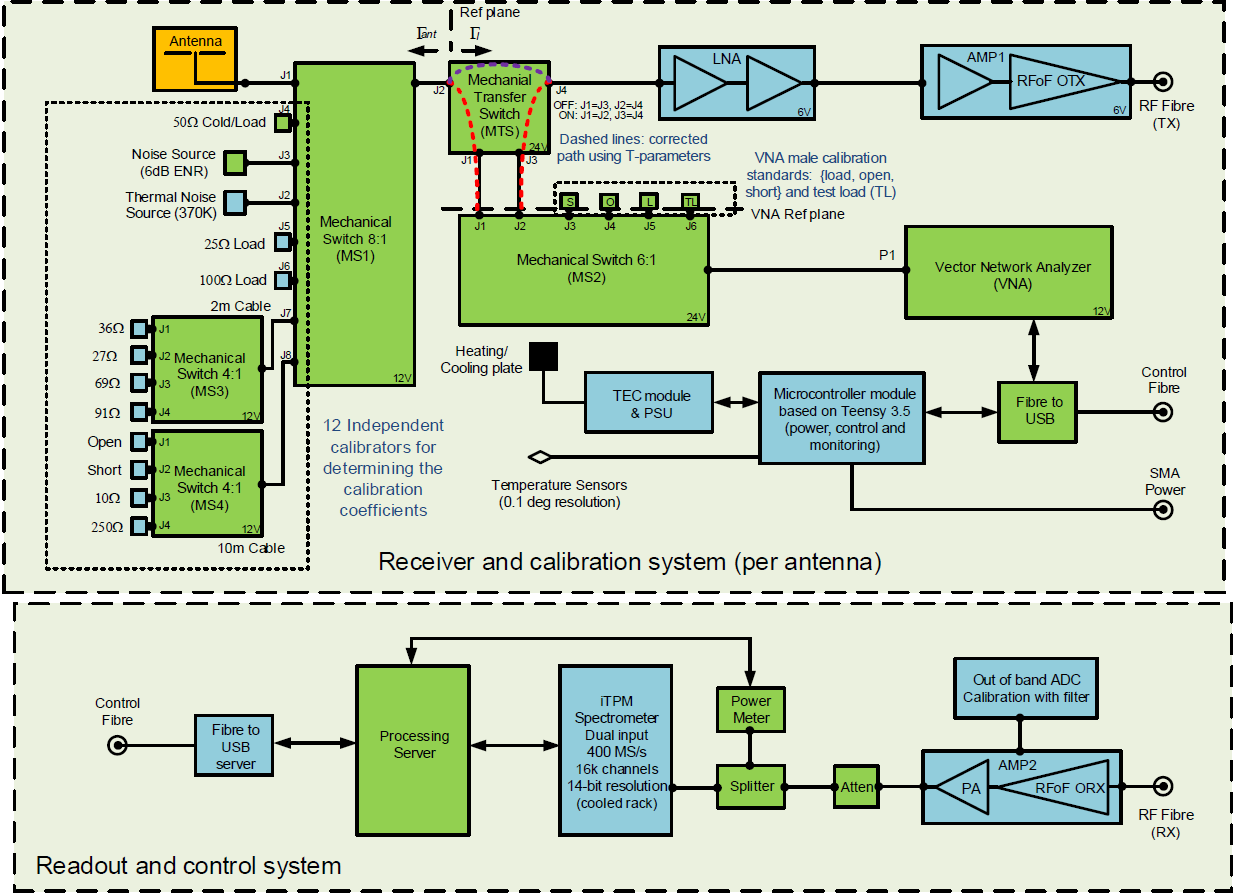
\includegraphics[width=\columnwidth]{radiometer_v8a}
    \caption{An overview of the REACH radiometer showing calibration sources and the antenna connected to an 8-way mechanical input switch at the receiver input. The green sub-blocks represent off-the-shelf components, whilst blue represent custom designs. $\Gam{ant}$ represents the reflection coefficient of the antenna or calibrator, $\Gam{l}$ is the reflection coefficient of the low noise amplifier (LNA). The red dashed line represents the extra path measured by the VNA that is not present during spectral measurements while the purple dashed line is the path present exclusively during spectral measurements. Corrections for these additional paths are detailed in \cref{sec:tparameters}. ‘ENR’ is the Excess Noise Ratio of a Noisecom NC346A noise source; ‘OTX’ indicates an optical transmitter; ‘TX’ indicates transmission mode; ‘TEC’ stands for Thermoelectric Cooling; ‘SMA’ is a SubMiniature version-A connector; ‘PA’ is Power Amplifier; ‘RX’ indicates reception mode and ‘Atten.’ represents a signal attenuator. Updated from figure included in \citet{reach}.}
    \label{fig:overview}
\end{figure}
As shown, a Mechanical Transfer Switch (MTS) facilitates pathways to the Low Noise Amplifier (LNA) and Vector Network Analyser (VNA) for spectral and reflection measurements respectively. MTS position two connects directly to the 8-way switch housing the calibration sources and MTS position four leads to the LNA/spectrometer pathway. The first and third MTS switch positions connect to the first two positions of a 6-way switch (MS2) that direct to the VNA. MS2 positions three through six connect to additional calibration standards used to separately calibrate the VNA before measurement as detailed in a following VNA subsection. For all of the connections detailed here, male sources and terminations were connected to female switch connections to avoid reflections that would spawn from the inclusion of male-female adaptors\footnote{or ‘worms’ as they are colloquially referred to.}

An effort was made to reduce any negative effects presented to the instrument by this network of switches. Mechanical switches were implemented over the alternative electronic switches due to the lower signal loss of the former. The Mini-Circuits absorptive switches chosen exhibit 0.01 dB loss within the REACH observational band with better than 100 dB isolation to reduce the radio-frequency leakage into the rest of the signal chain. Extra shielding was added to the switch drivers to further reduce self-induced RFI as shown in \cref{fig:switches}. The 20 mm trace length of the mechanical switch drivers was mitigated by placing the drivers as close to the switch as possible followed with the inclusion of custom 3D-printed connection covers coated with conductive paint.
\begin{figure}
    \centering
    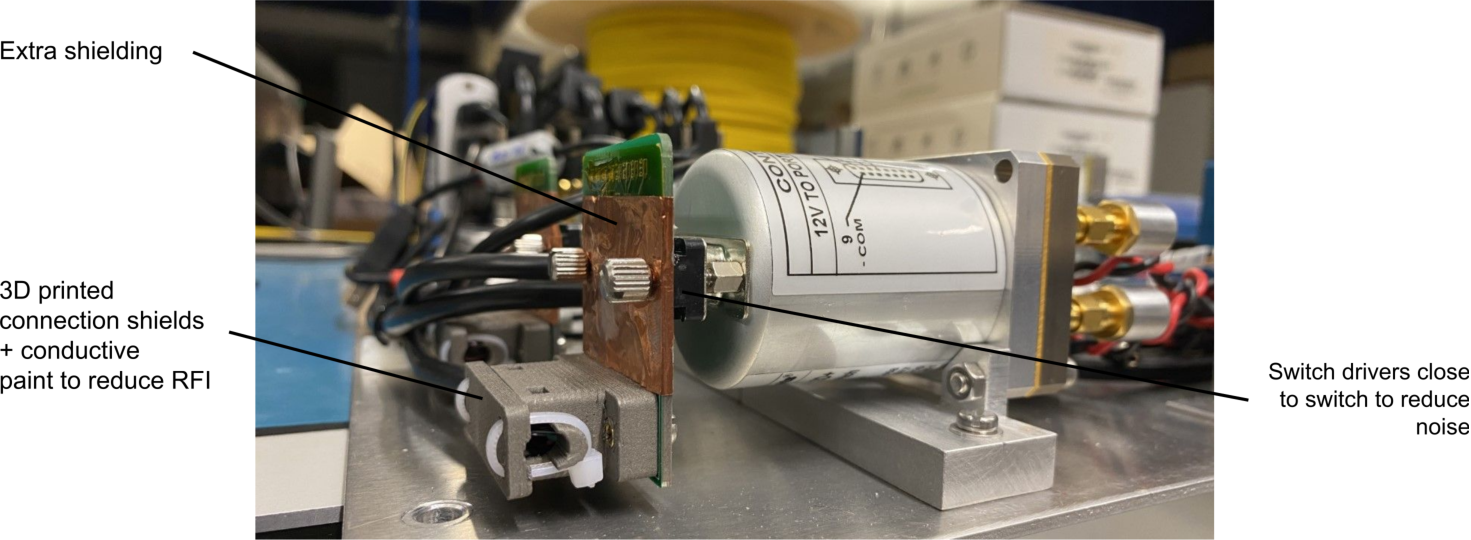
\includegraphics[width=\textwidth]{switches}
    \caption{A mechanical switch installed on the front-end component plate showing the extra shielding, 3D-printed housing and close placement of switch drivers.}
    \label{fig:switches}
\end{figure}
A table of the mechanical switches used is presented in \cref{tab:switches} for reference and a table with the contents of each switch connection detailed in \cref{tab:switch_content}. An mock-up of the switch configuration for a reflection coefficient measurement of the open-ended 10 metre cable is provided in \cref{fig:switch_mock} for illustrative purposes as well.
\begin{figure}
    \centering
    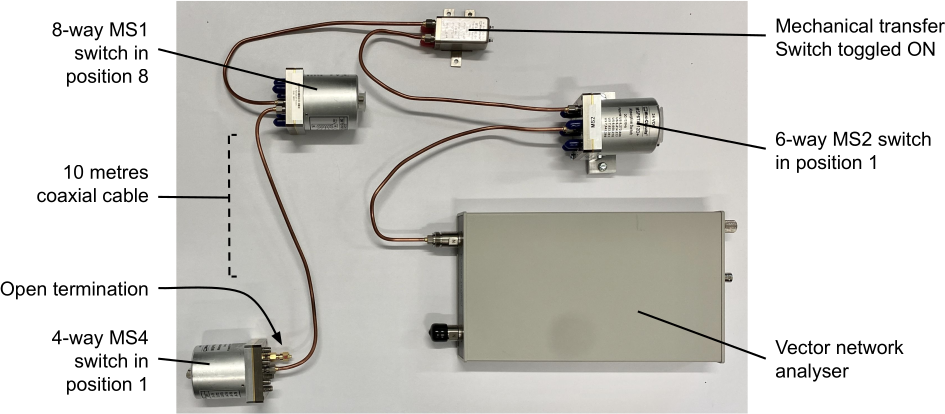
\includegraphics[width=\textwidth]{switch_example}
    \caption{A mock-up of the components and configuration needed for a reflection coefficient measurement of the open-ended 10 metre cable using parts from the receiver (except for the 10 metre cabling which was too long.). For this measurement, the open termination connected to the MS4 switch input port 1 with the MS4 switch toggled to position 1 via command line interface. The MS4 switch output is connected to the 10 metres of LMC195 cabling with the other end of the LMC195 cable connected to the port 8 input of the MS1 switch. The MS1 switch is toggled to position 8 via CLI. The MS1 output connects to the port 2 input of the MTS switch followed by a connection to the port 1 input of the MS2 switch. With the MS2 switch toggled to port 1, the MS2 output should connect to the VNA input allowing for a connection to the opened termination though the MS2, MTS, MS1 and MS4 switches. This configuration allows for a reflection coefficient measurement of the opened termination by the VNA.}
    \label{fig:switch_mock}
\end{figure}


% =========================================
\subsubsection{The microcontroller unit}
As with most modern instruments, control an monitoring of the receiver front-end and its individual components is overseen by a central device. This control unit is required to initialise the specific switch positions needed for measurements as seen in \cref{fig:overview}. As an unmanned experiment in the South African Karoo, the capability for resetting components, especially during remote triage, is another critical function of the controller unit. With 88 necessary connections to oversee within the receiver front-end, construction of an adequate controller using off-the-shelf components would ordinarily take the space of a standardised 19-inch rack ($\sim 48$ cm\textsuperscript{2}). This along with the low noise requirements and restricted power budget of the REACH experiment prompted the development of a novel control unit design; a miniaturised management device or, ‘microcontroller unit’\footnote{Also abbreviated as ‘$\mu$con’ for short.}. Much of the compactness of our miniaturised control unit can be attributed to a careful consideration in constituent components however, an innovative stacked dual-board design allowed us to reduce the size by an order of magnitude condensing the microcontroller unit into a $13 \times 12 \times 10$ cm volume.

The first of the two boards in our microcontroller unit is the control board mounted by a PJRC Teensy 3.5 development board\footnote{Teensy 4.X is suggested for any future receiver designs due to the anticipated permanent reduction in supply of the 90 nm silicon MK64FX512VMD12 chips constituent to the Teensy 3.5. Newer Teensy boards boasting 45 nm chips may also provide increased efficiency and capability in subsequent builds.} based on the Arduino infrastructure. The Teensy board, as shown in \cref{fig:teensy} contains 64 digital input/output ports assigned to individual switch configurations facilitating component control through a USB serial interface.
\begin{figure}
    \centering
    \begin{subfigure}{0.5\textwidth}
        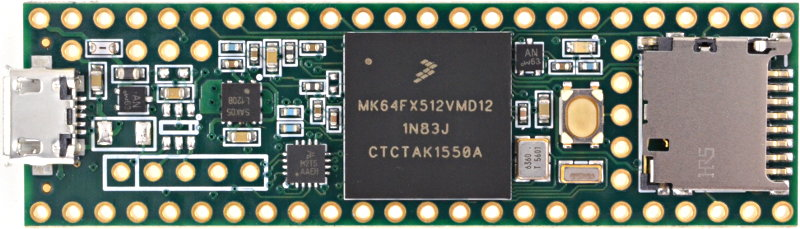
\includegraphics[width=\textwidth]{teensy_top}
    \end{subfigure}
    \begin{subfigure}{0.5\textwidth}
        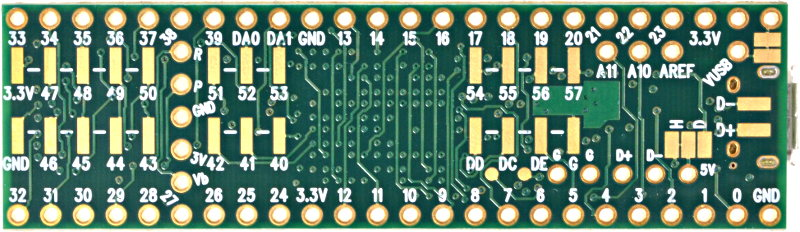
\includegraphics[width=\textwidth]{teensy_bottom}
    \end{subfigure}
    \caption{The front and back of the Teensy board is shown in the top and bottom respectively. Along the edges of the board are the input/output connectors (yellow-outlined white circles) which are paired to specific mechanical switch configurations throughout the front-end. Image taken from PJRC website: \url{https://www.pjrc.com/store/teensy35.html}.}
    \label{fig:teensy}
\end{figure}
The $110 \times 90$ mm control board upon which the Teensy board is mounted to also contains the 48 V power input from the solar panels as well as 12 V and 5 V outputs for front-end components and can be seen in \cref{fig:control_board}.
\begin{figure}
    \centering
    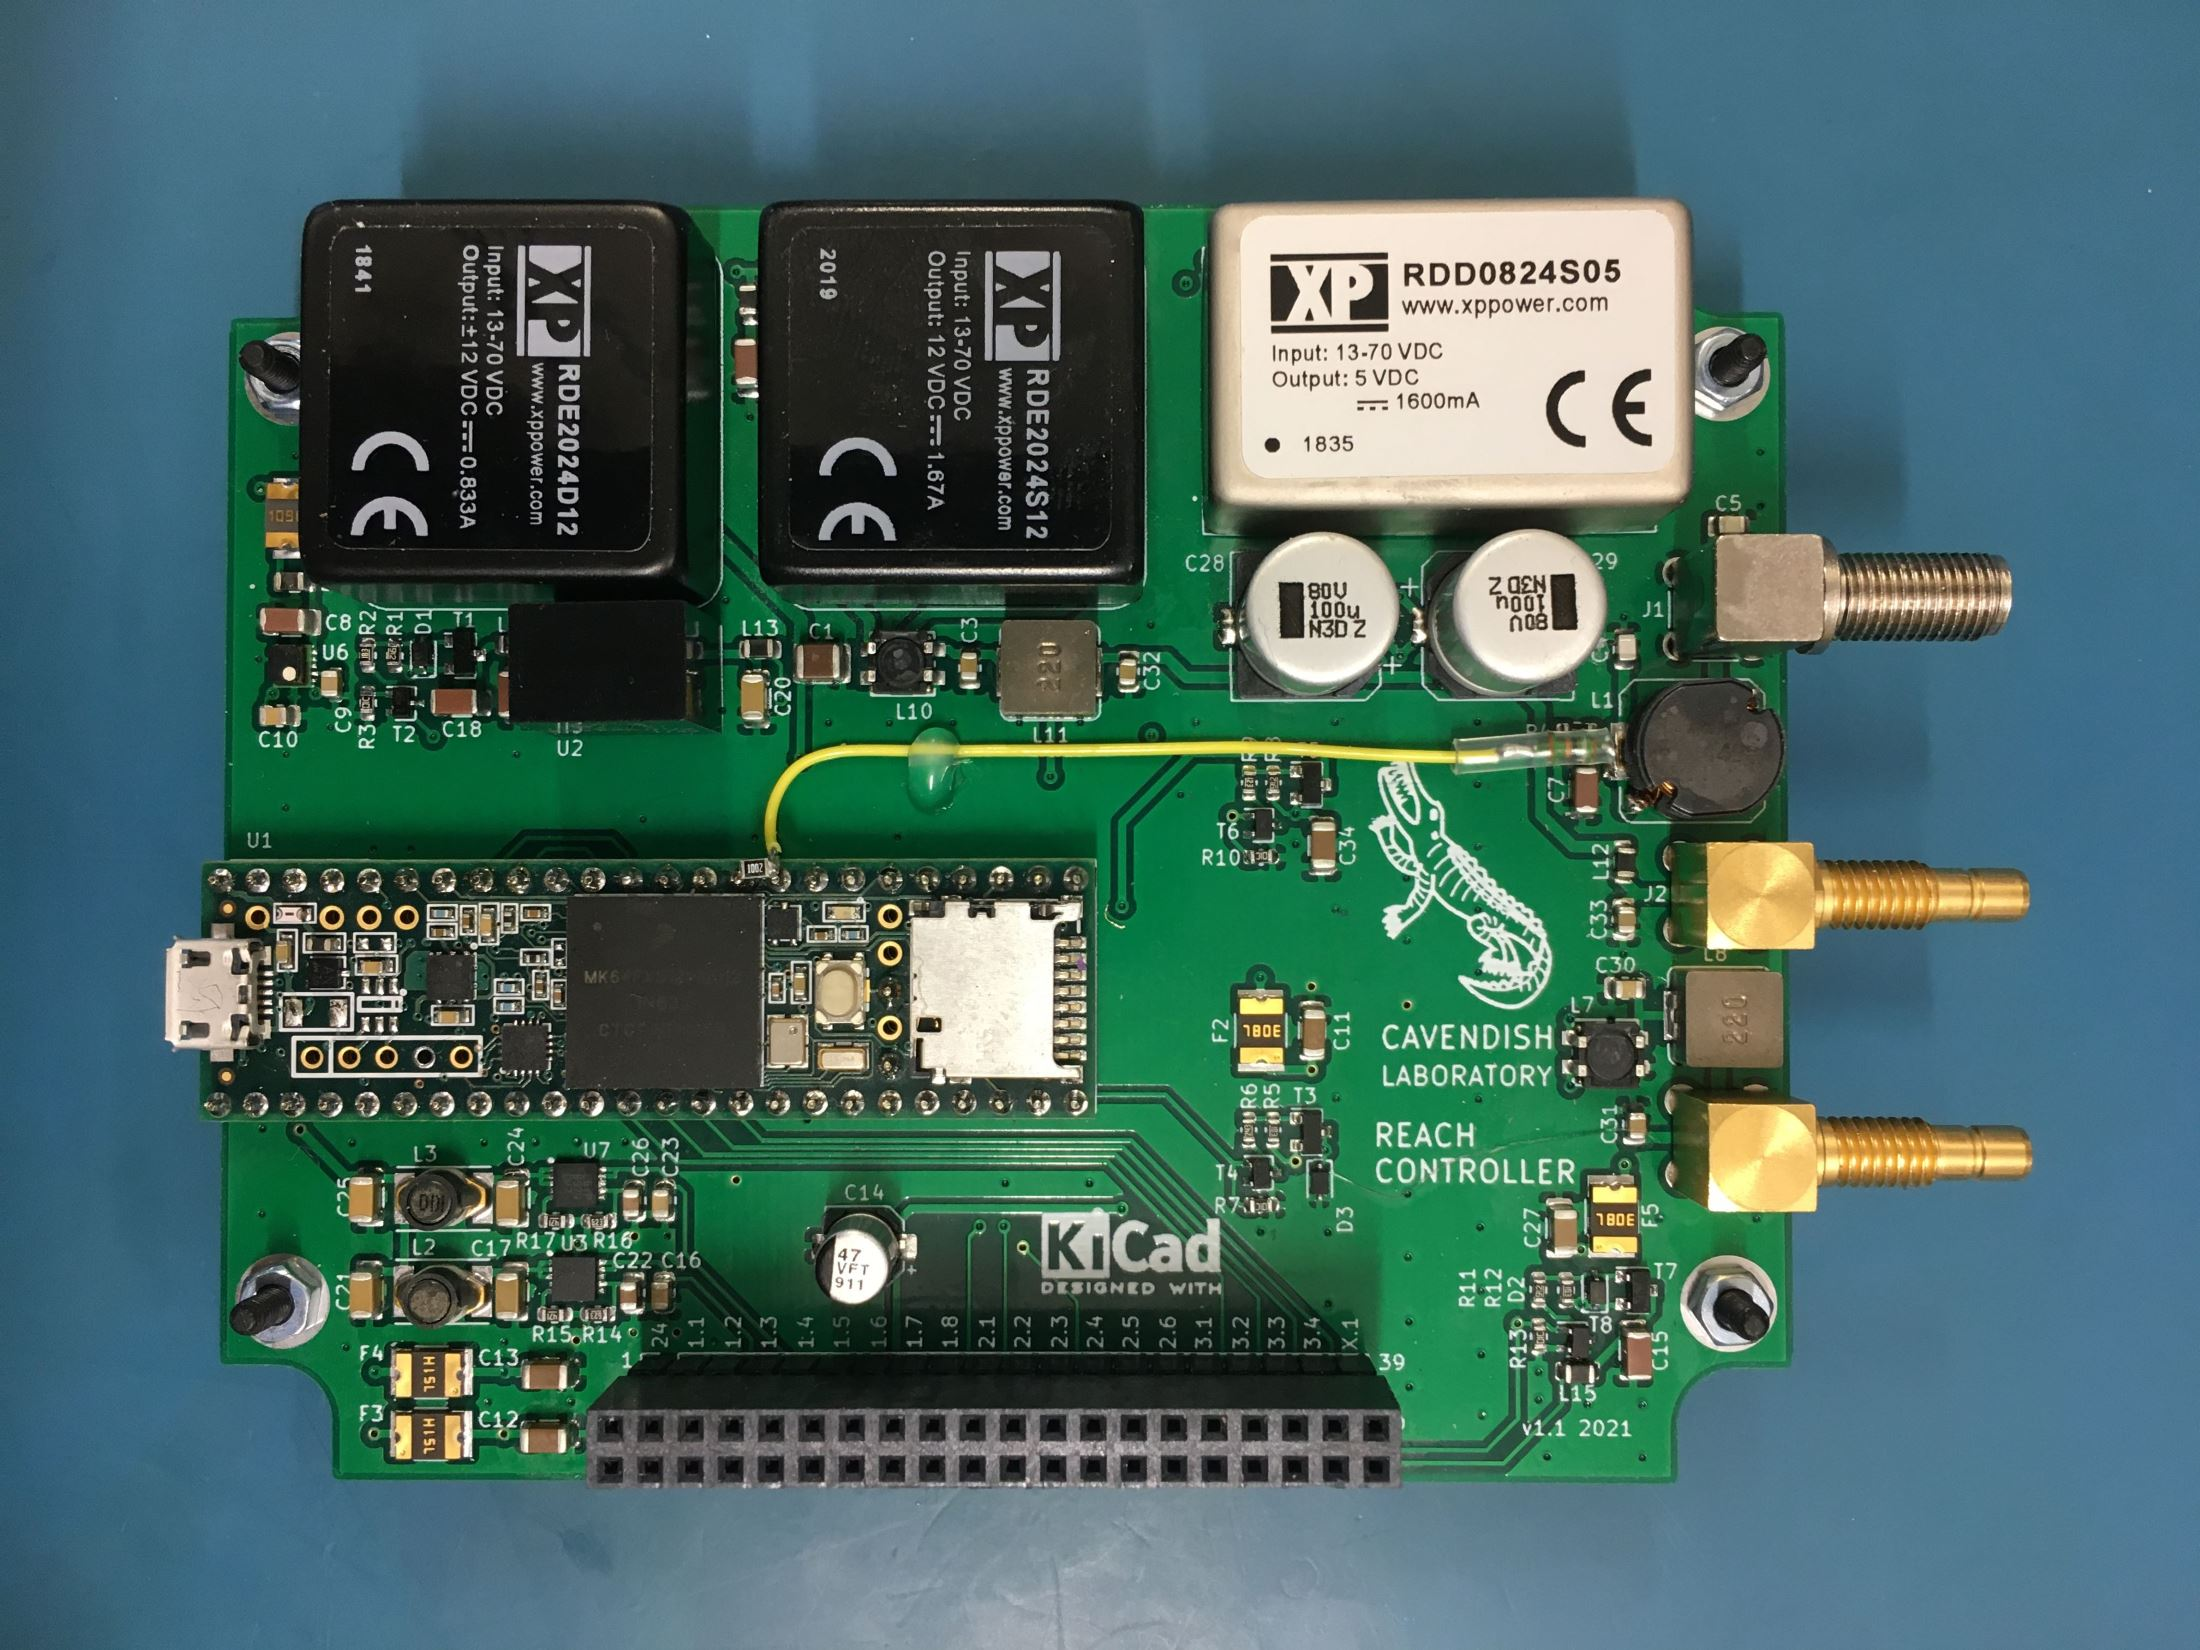
\includegraphics[width=0.5\textwidth]{control_board}
    \caption{The microcontroller unit control board with the Teensy board mounted at the left centre. The 48 V in, 12 V and 5 V out can be seen on the right of the board serving a portion of the overall microcontroller unit's power distribution functionality.}
    \label{fig:control_board}
\end{figure}
The controller board also incorporates RFI filtering and I\textsuperscript{2}C bus subsystems for ancillary device control such as the external fan.

Stacked above the controller board is the breakout board as shown in \cref{fig:break_board} which is primarily responsible for the remaining front-end connections but also a 28 V noise source regulator, 6 V power supply and additional EMI filtering.
\begin{figure}
\centering
    \centering
    \begin{subfigure}{.5\textwidth}
        \centering
        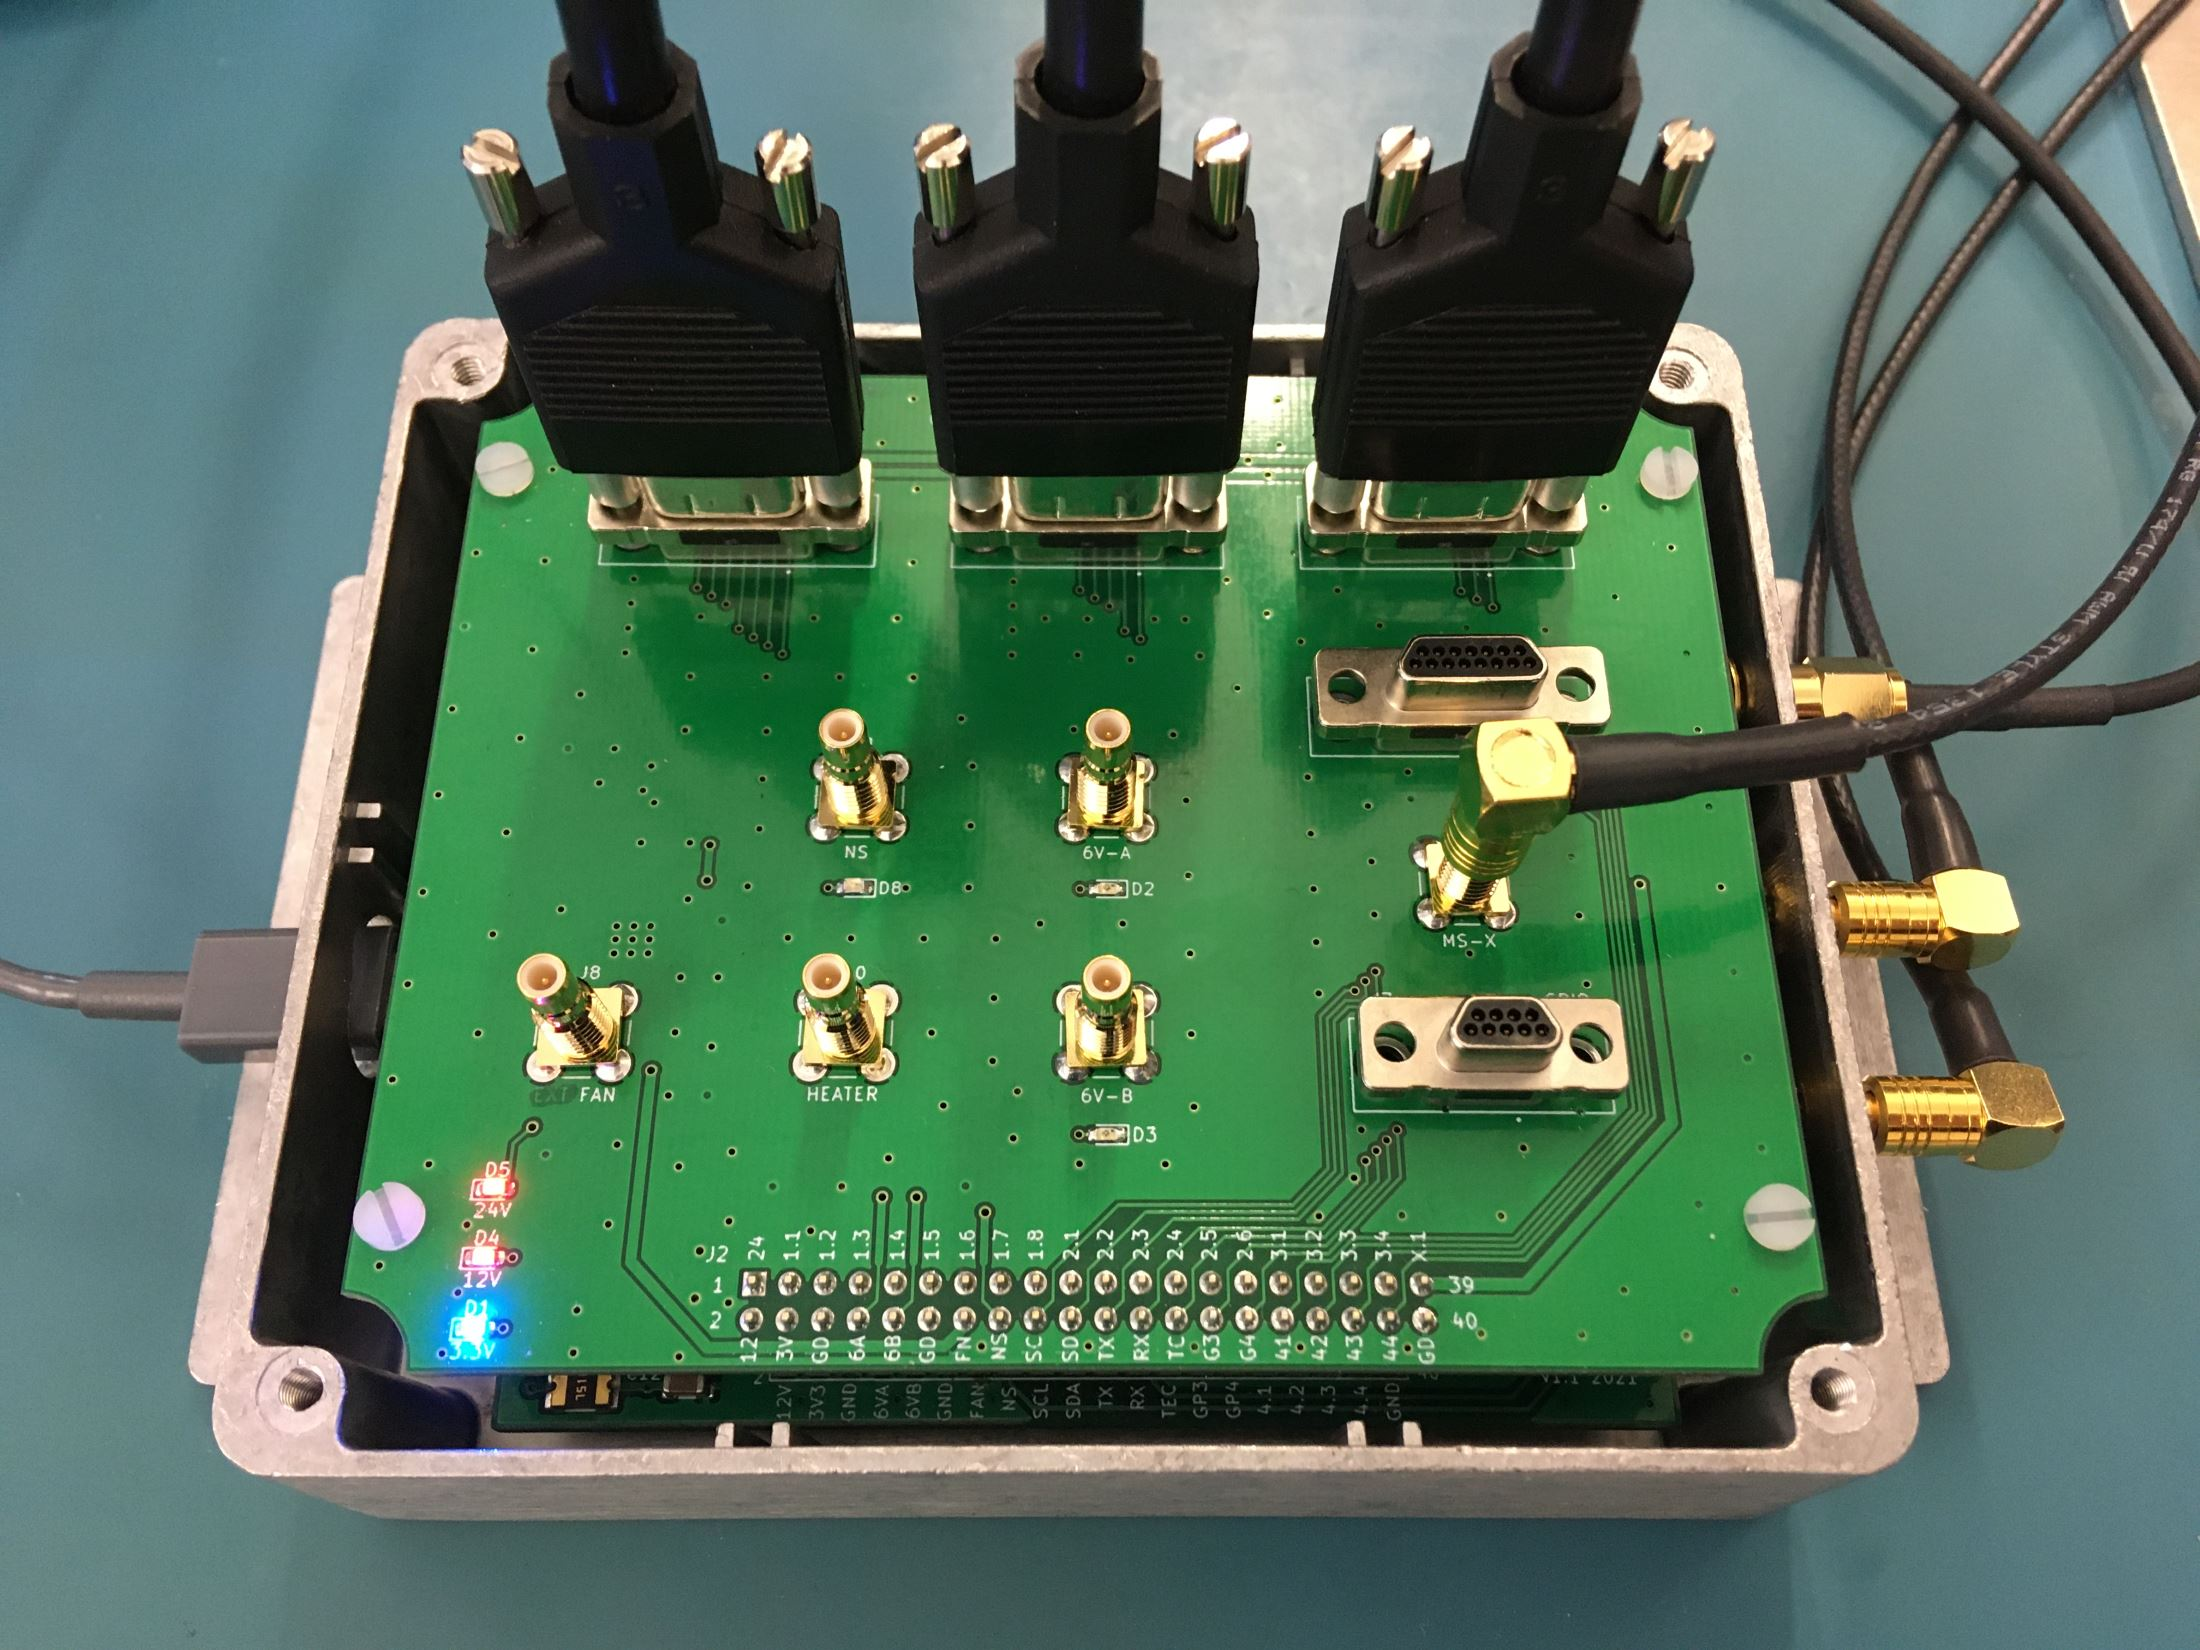
\includegraphics[width=\linewidth]{ucon}
    \end{subfigure}
    \hfill
    \begin{subfigure}{.45\textwidth}
    \centering
        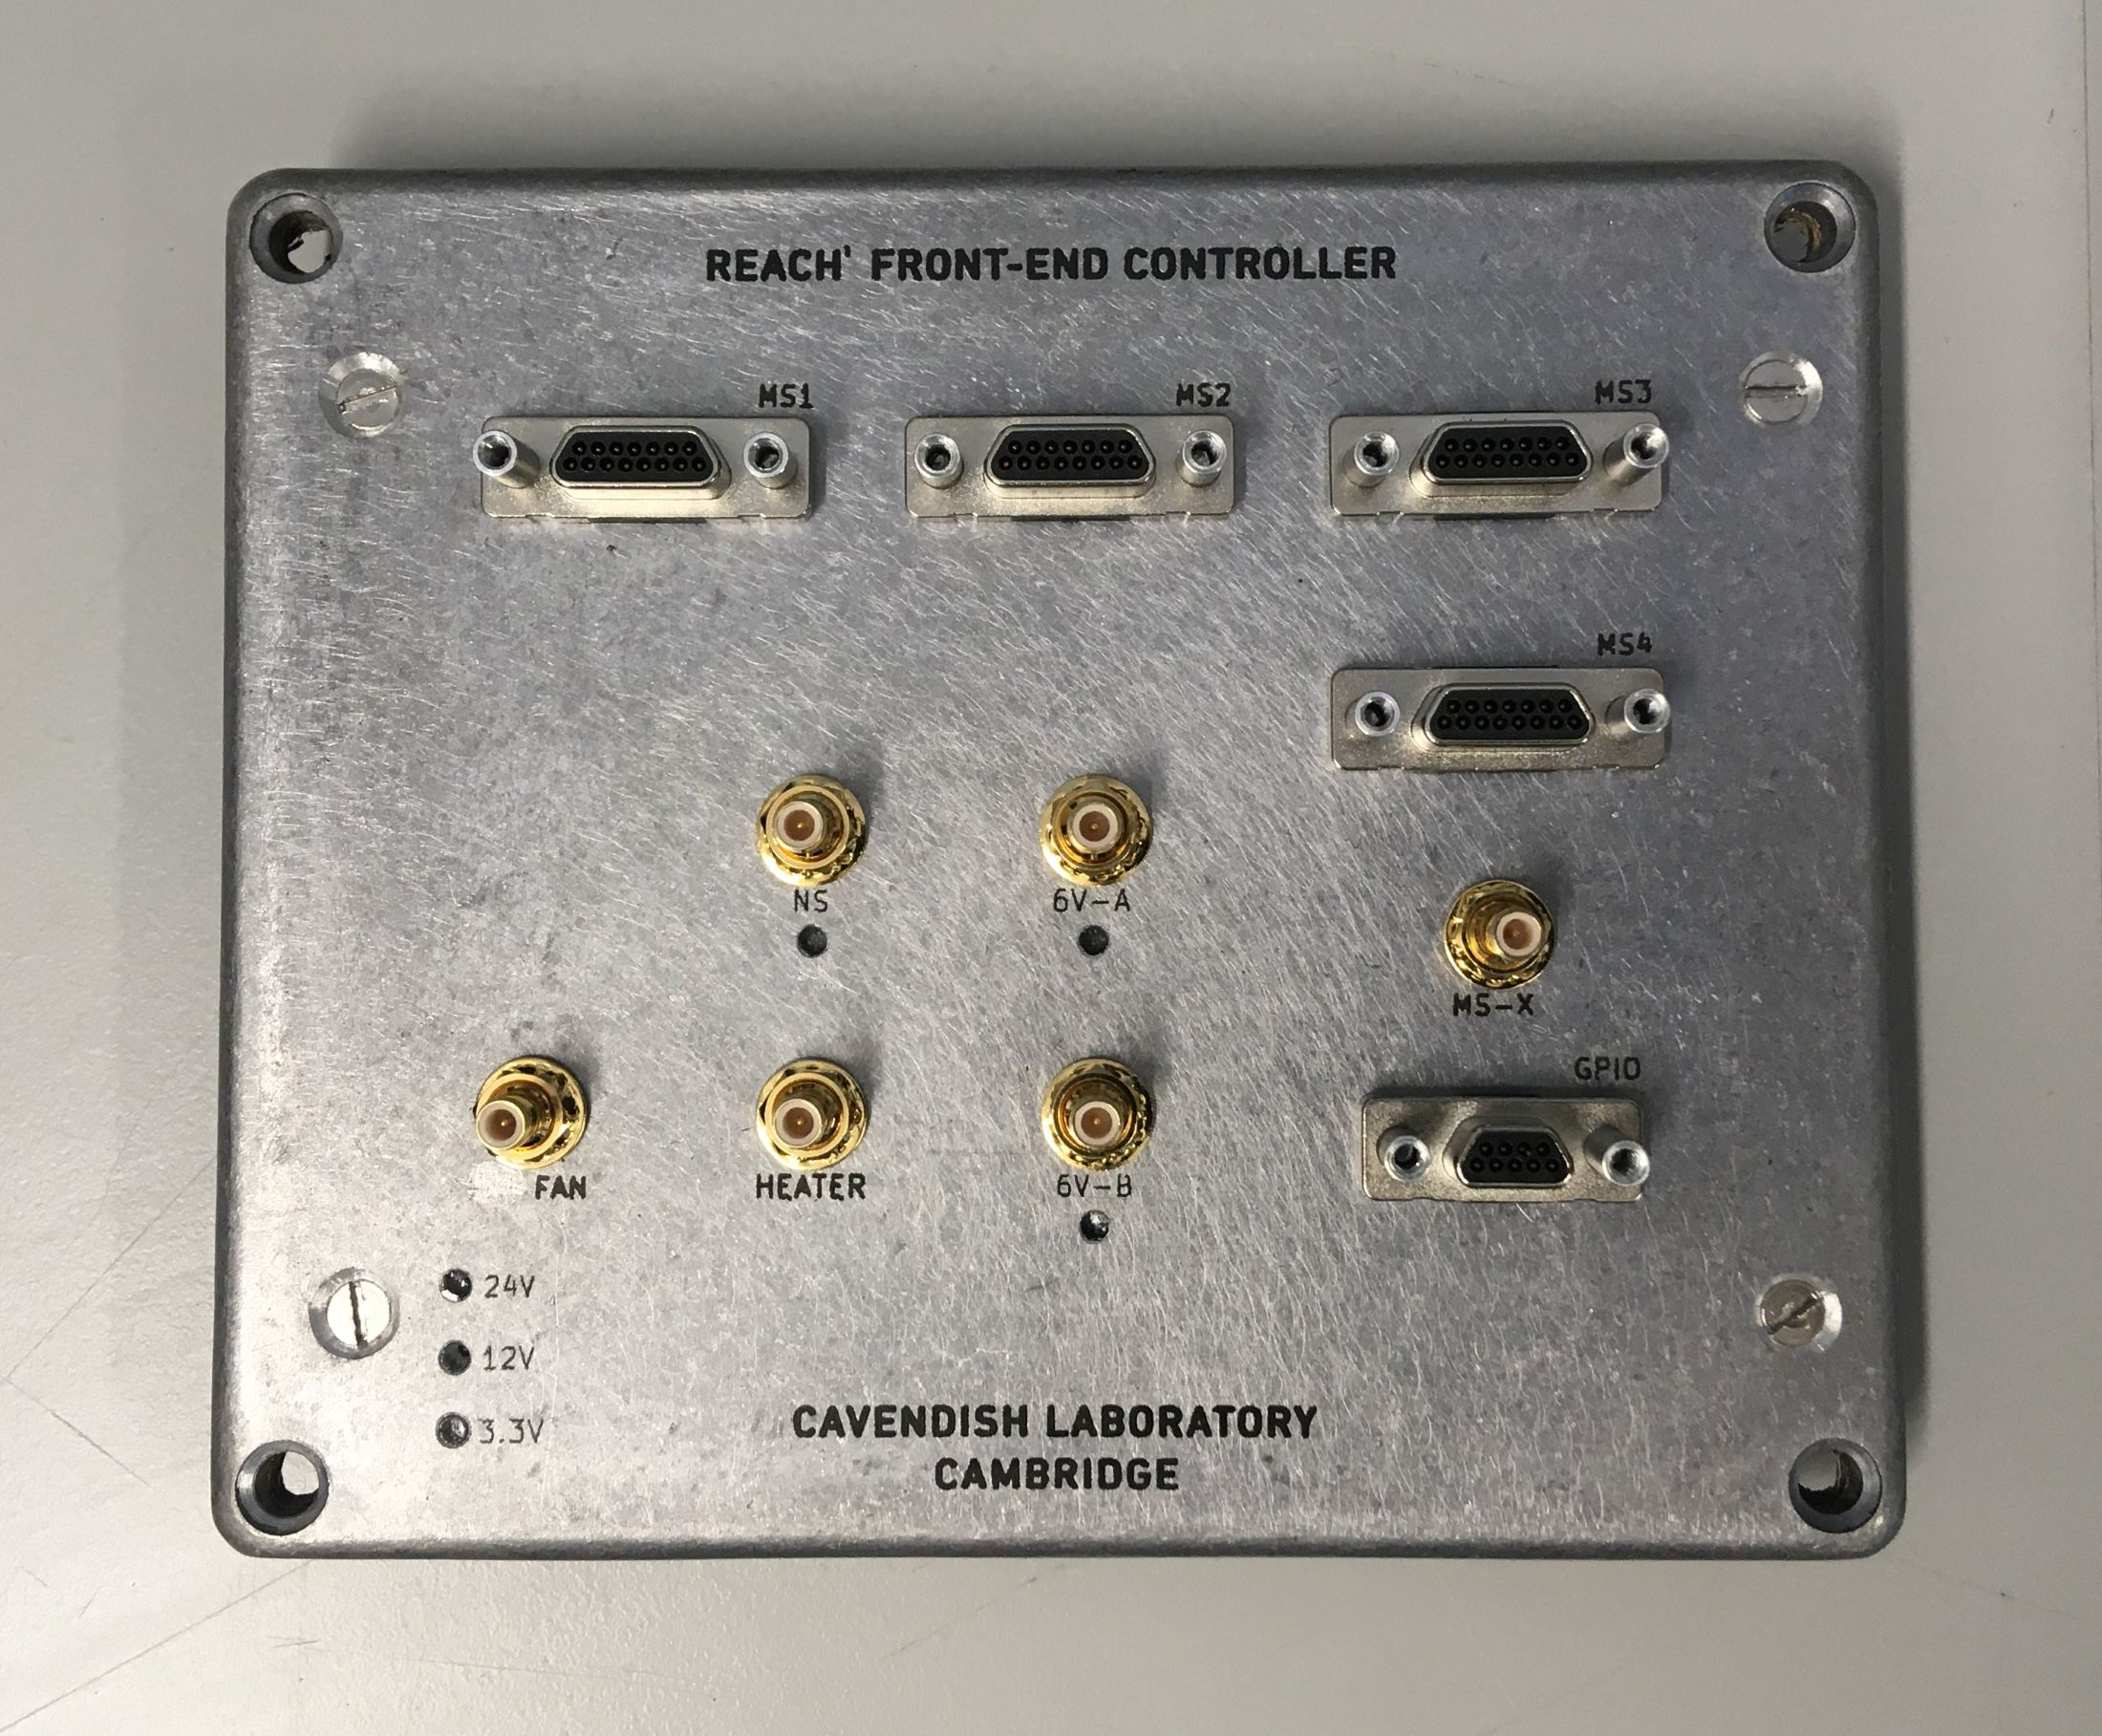
\includegraphics[width=\linewidth]{ucon_cover}
    \end{subfigure}
    \caption{The breakout board of the microcontroller is shown on the right displaying the mechanical switch connections across the top row. The remaining power supply connections can also be seen on the board. The top cover of the completed microcontroller unit is shown on the right with laser markings annotating the connections of the breakout board. Image credit: Steven H. Carey.}
    \label{fig:break_board}
\end{figure}
A CAD rendering depicting the stacked microcontroller unit is also shown as \cref{fig:ucon_cad}.
\begin{figure}
    \centering
    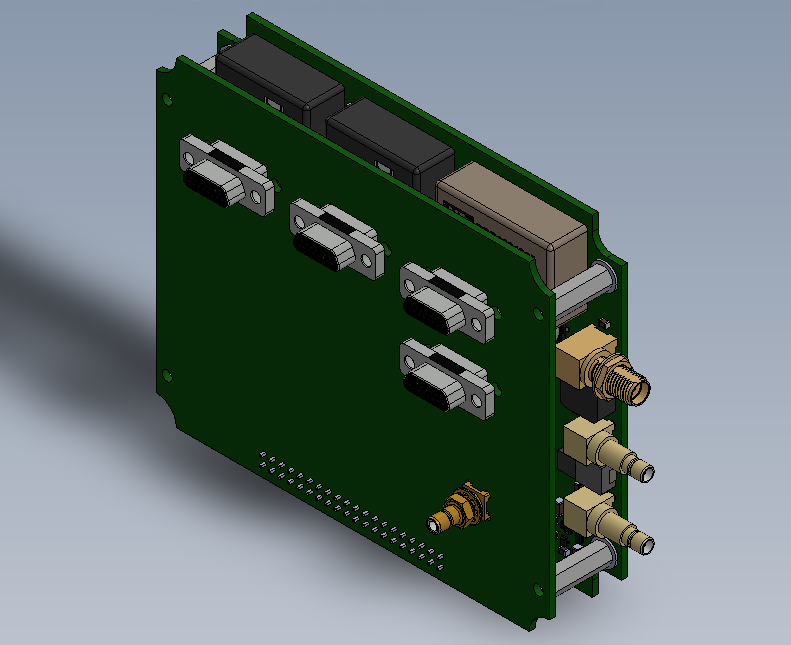
\includegraphics[scale=0.4]{stacked_ucon}
    \caption{A rendering of the microcontroller assembly showing the breakout board seated above the controller board both outside the microcontroller housing. Also not shown is a heat transfer bracket between the three converter modules. The staked design of the microcontroller allowed for the small form factor required by the REACH experiment. CAD rendering credit: Steven H. Carey.}
    \label{fig:ucon_cad}
\end{figure}
The completed unit supplies power to every component within the front-end except for the thermal management system which has its own power supply unit as previously detailed. A combination of switched-mode power supply (SMPS) and linear regulators are employed to optimise both low noise and efficiency with the six DC-DC power supplies having an efficiency of at least 85\%. A table detailing the power supplies managed by the microcontroller unit is shown in \cref{tab:power_supply}. Further conductive gaskets were placed under bulkhead connectors for additional noise reduction and additional DC filtering is provided on the 48 V input supply. A block diagram of the completed microcontroller unit is provided in \cref{fig:ucon_block}.
\begin{figure}
    \centering
    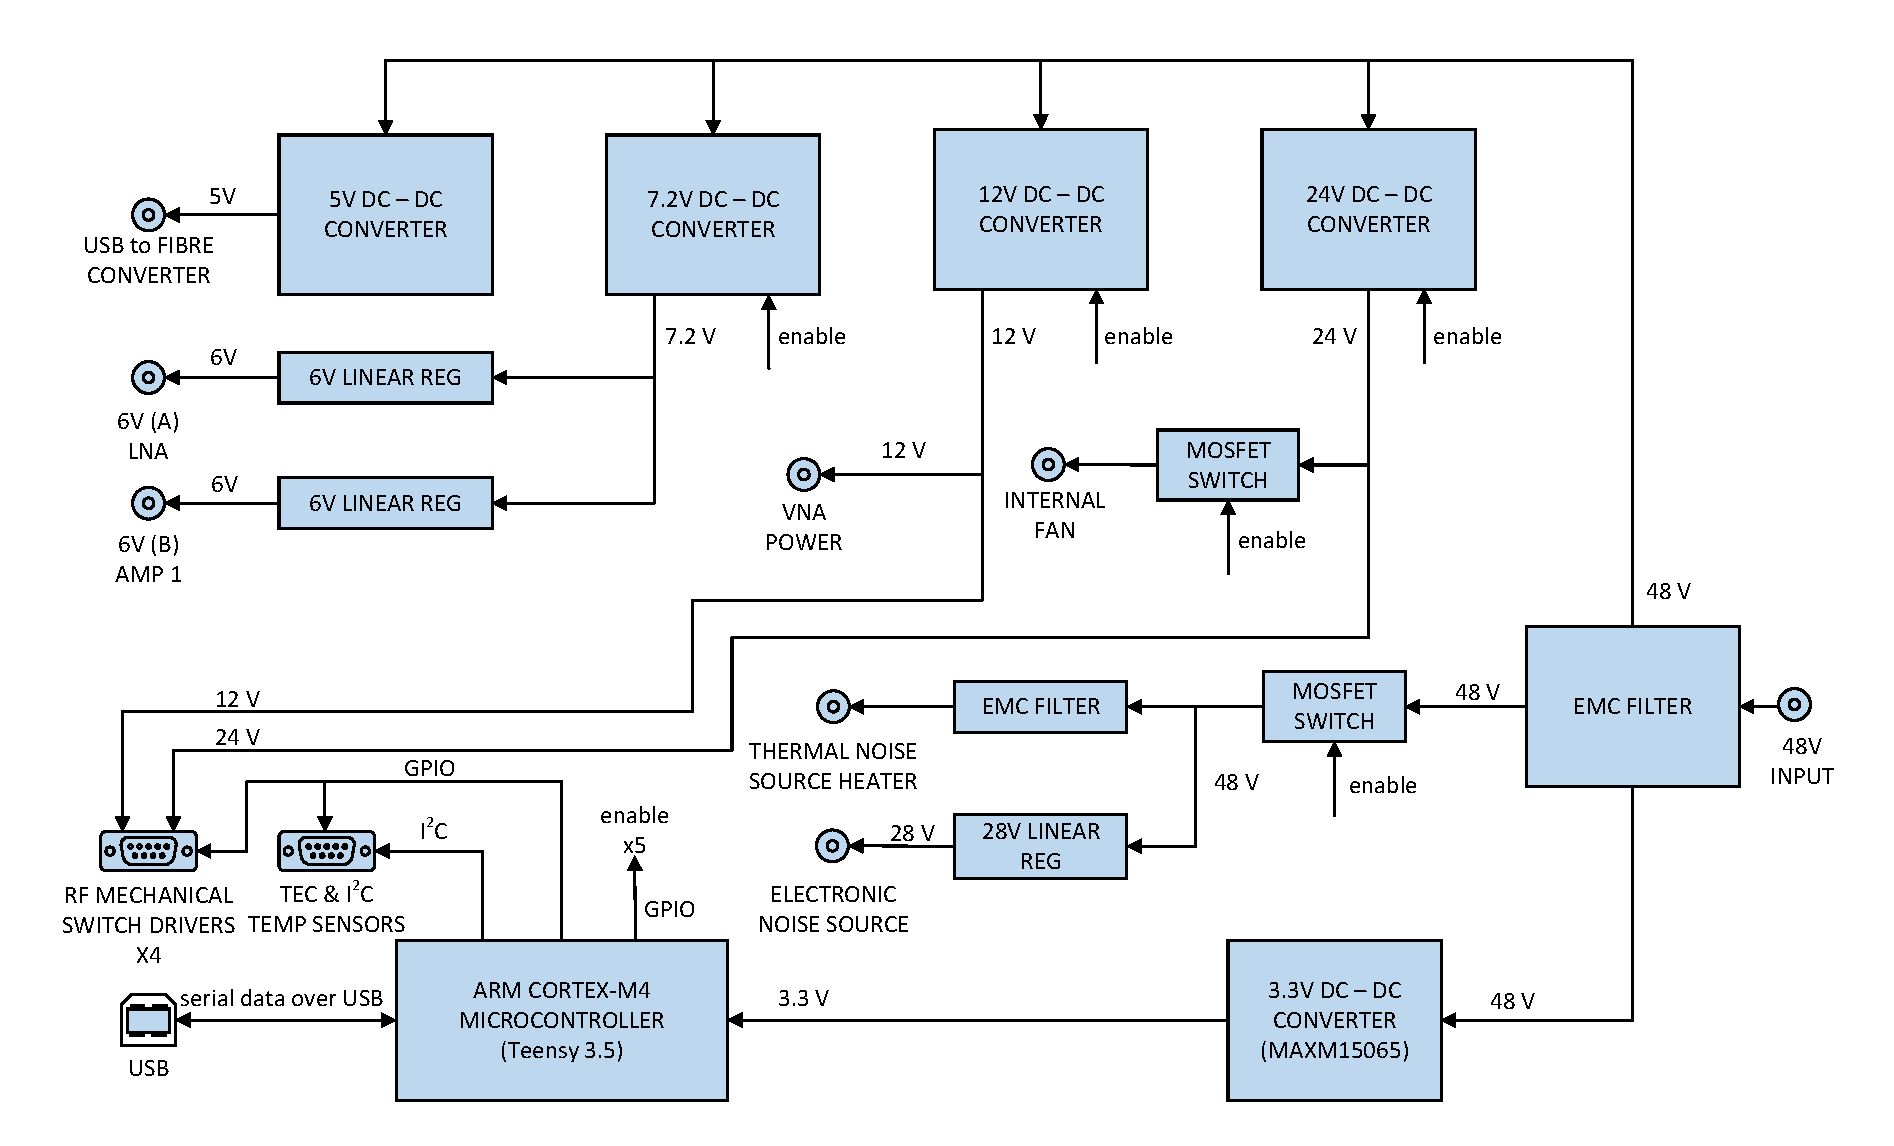
\includegraphics[width=\textwidth]{updated_controller_detail}
    \caption{A detailed microcontroller block diagram showing the components, connections and power considerations incorporated into the design.}
    \label{fig:ucon_block}
\end{figure}
The completed unit demonstrates a high efficiency with a 2 K temperature rise seen within the microcontroller casing with all supplies on at full load.


% =========================================
\subsubsection{Temperature measurement via thermocouple}
Within the receiver front-end are probes measuring the temperatures of various components needed for calibration. Initial designs utilised eight Microchip Technology MCP9808 temperature sensors that communicate directly with the microcontroller unit using I\textsuperscript{2}C protocol over the Arduino command line interface. Thermal gap pads would be used to thermally bond the 2-centimetre-wide temperature sensors to front-end components yielding an accuracy of $\pm 0.5$ K. The I\textsuperscript{2}C sensors’ native connection to the microcontroller unit conformed to the space restrictions of the front-end enclosure however, it was decided that smaller probe tips for placement on individual components as well as additional temperature sensors would increase the accuracy of our calibration prescription. A Pico Technology TC-08 Thermocouple Data Logger, shown in \cref{fig:tc08}, was employed to accommodate eight more temperature measurements using Pico Technology SE000 K-type thermocouples with TC-08 0.60 mm tip ends thermally bonded to components using RTV Thermally Conductive Oxime made by Electrolube.
\begin{figure}
    \centering
    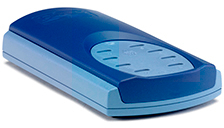
\includegraphics[width=0.4\textwidth]{tc08}
    \caption{The Pico Technology TC-08 Thermocouple Data Logger for use with eight K-type thermal probes. Image taken from Pico Technology website: \url{https://www.picotech.com/data-logger/tc-08/thermocouple-data-logger}.}
    \label{fig:tc08}
\end{figure}
The simple incorporation of the TC-08 with our receiver automation software through the manufacturer’s proprietary Python libraries also factored into our decision to use the device. The TC-08 thermocouples have an accuracy of $\pm 1.1$ K\footnote{Sum of $\pm0.2$\% of reading and $\pm0.5$ K according to manufacturer specifications.} for our measurements typically around 300 K and relay information to the back-end server via USB connection at a cadence of one measurement every 10 seconds. A table of the TC-08 Data Logger port assignments is shown in \cref{tab:tc08}\footnote{These port assignments are representative of the front-end configuration at the time of shipment to South Africa in December 2022 and are subject to change.}.
\begin{table}
    \begin{center}
    \begin{tabular}{ |c|c| }
    \hline
    TC-08 Port Number & Component \\
    \hline
    Port 0 & Cold Junction \\
    Port 1 & MS1 switch \\
    Port 2 & Heated load thermistor \\
    Port 3 & MS3 switch\\
    Port 4 & MS4 switch \\
    Port 5 & 2 metre calibration cable \\
    Port 6 & 10 metre calibration cable \\
    Port 7 & Low noise amplifier \\
    Port 8 & Antenna (laboratory) \\
    \hline
    \end{tabular}
    \caption{The port assignments for the TC-08 connecting to various components within the receiver front-end. The Port 2 thermocouple was attached to the thermistor end of the simplified heated load construction. The Port 5 and 6 probes were connected directly to the outside of the calibration cables for measurement of the physical cable temperature with the terminating sources assumed to be at the same temperature as their respective switches. In the Cambridge laboratory, the Port 8 thermocouple was fed through a small hole drilled through the wall of the front-end enclosure and attached to the end of a makeshift antenna used for testing of the calibration algorithm.}
    \label{tab:tc08}
    \end{center}
\end{table}

We highlight that Port 0 of the TC-08 lists a ‘Cold Junction’ which is the temperature of the Data Logger unit itself and not the similarly named ambient temperature ‘cold’ load. Furthermore, the position of the MCP9808 I\textsuperscript{2}C temperature sensors were not finalised or thermally bound to anything by the time of deployment in August 2023 though it is envisioned that measurements of additional components needed for the temperature corrections detailed in \cref{sec:cable_gradient} are the primary responsibility of the I\textsuperscript{2}C sensors. The temperature stability of various sources recorded by the TC-08 are shown in \cref{fig:temperature}.
\begin{figure}
    \centering
    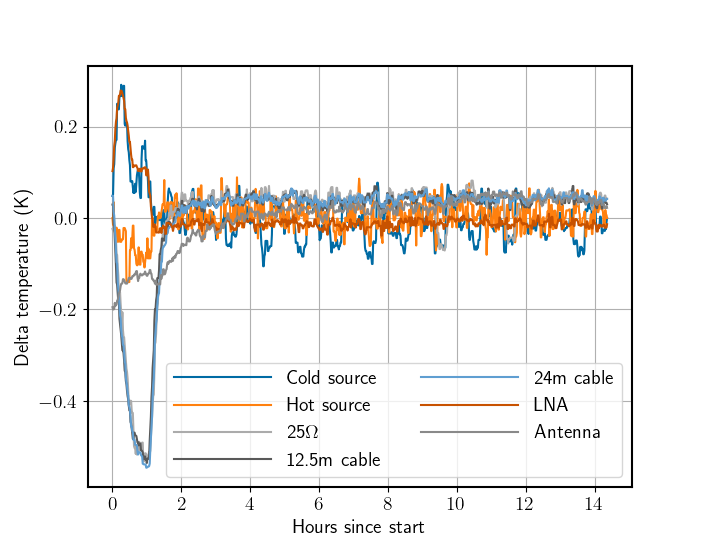
\includegraphics[scale=0.6]{temperature}
    \caption{Receiver component temperature stability recorded by the TC-08 Data Logger. The fluctuations seen within the first two hours of the measurements are from mechanical switch stabilisation and the VNA calibration procedure. We highlight the temperature stability of the individual components after environmental stability is achieved. The plot includes measurements of the 12.5 metre and 24 metre calibration cables before being replaced by the 2 metre and 10 metre cables as detailed in Calibration sources subsection. Image credit: Prof. Alessio Magro.}
    \label{fig:temperature}
\end{figure}


% =========================================
\subsubsection{Vector Network Analyser}
Reflection coefficients of the calibration sources, LNA and antenna are measured with a Copper Mountain Technologies TR1300/1 2-port 1.3 GHz vector network analyser (VNA) shown in \cref{fig:vna}.
\begin{figure}
    \centering
    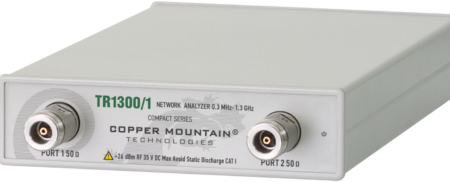
\includegraphics[scale=0.5]{vna}
    \caption{Copper Mountain Technologies TR1300/1 Vector Network Analyser. Image taken from Copper Mountain Technologies website: \url{https://coppermountaintech.com/vna/tr1300-1-2-port-1-3-ghz-analyzer/}.}
    \label{fig:vna}
\end{figure}
The main consideration for including this VNA model was the small $28.5 \times 14.2 \times 4$ cm form factor for inclusion in the front-end enclosure. The VNA measurement accuracy as provided by the manufacturer is shown in \cref{tab:vna_acc}.
\begin{table}
    \begin{center}
    \begin{tabular}{ |c|c| }
    \hline
    Reflection measurement & Accuracy (Magnitude) \\
    \hline
    -15 dB to 0 dB & $\pm$0.4 dB \\
    -25 dB to -15 dB & $\pm$1.5 dB \\
    -35 dB to -25 dB & $\pm$4.0 dB \\
    \hline
    \end{tabular}
    \caption{Manufacturer quoted measurement accuracies for the Copper Mountain Technologies TR1300/1 Vector Network Analyser.}
    \label{tab:vna_acc}
    \end{center}
\end{table}

Reflection coefficient measurements of various receiver components is shown in \cref{fig:s11_meas}. 
\begin{figure}
    \centering
    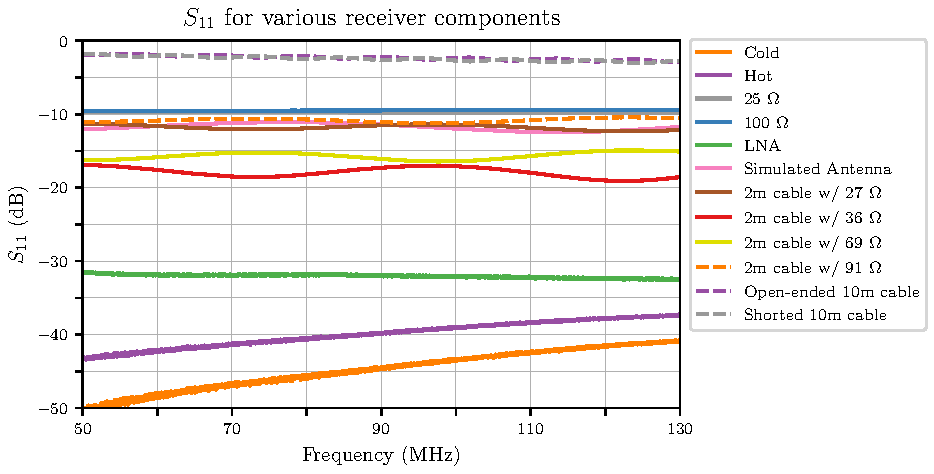
\includegraphics[width=\columnwidth]{s11_meas}
    \caption{Reflection coefficients for various receiver components including the LNA and simulated antenna.}
    \label{fig:s11_meas}
\end{figure}
Upon inspection of \cref{tab:vna_acc}, one may note that the VNA is not rated for extremely low reflection measurements below -35 dB such as the ambient temperature and heated $50\Omega$ loads shown in \cref{fig:s11_meas}. In order to quantify the quality of our measurements in this low-reflection regime, we use the manufacturer provided data of \cref{tab:vna_acc} and calculate a spread in $\pm$dBs representing our measurement error for the regions our machine is rated for. We then convert this spread from dB to linear using
\begin{equation}
    \mathrm{measurement \ spread} = 10^{\frac{\mathrm{measurement} + \mathrm{error}}{10}} - 10^{\frac{\mathrm{measurement} - \mathrm{error}}{10}}.
    \label{eq:vna_spread}
\end{equation}
The linear measurement spreads are plotted in \cref{fig:vna_acc} where we have fitted the manufacturer provided data with a decaying exponential using \textsc{SciPy.optimize} and extrapolated to the ranges applicable to the 50$\Omega$ loads. \begin{figure}
    \centering
    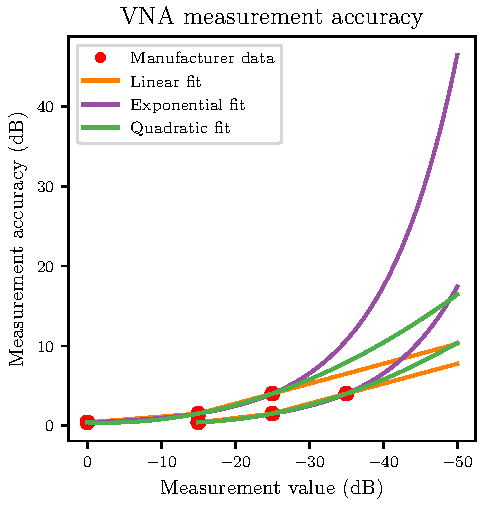
\includegraphics{vna_accuracy}
    \caption{VNA accuracy extrapolated to an extended measurement range for linear, exponential and quadratic fits to the manufacturer-provided data as shown in \cref{tab:vna_acc}. For $S_{11}$ measurements at levels as low as -50 dB, we regard a measurement accuracy of $\pm 15$ dB to be reasonable from comparison of the extrapolated fits.}
    \label{fig:vna_acc}
\end{figure}
For reflection coefficient measurements $\sim -45$ dB, we find a linear measurement spread of 0.002 corresponding to a VNA accuracy of $\pm$10 dB. In the logarithmic scale of dBs, this measurement accuracy is acceptable. A similar exercise of fitting a polynomial curve to the manufacturer provided data in the dB scale gives a similar but less conservative value for extrapolated measurement accuracy. We note that future iterations of the receiver front-end may benefit from inclusion of a VNA rated for low-reflection measurements but the small form factor of the TR1300/1 may be difficult to achieve.

A Python script using SCPI commands was developed in order to interact with and automate the VNA. This included a separate process to calibrate the VNA itself before proceeding with calibration of the receiver. VNA calibration was undertaken using short, open and load (SOL) standards from another Kirkby 85033 50$\Omega$ SMA calibration kit to maximise measurement accuracy of the reflection coefficients throughout a 50–-200 MHz band. The VNA calibration is tested against an additional $50\Omega$ test load that was measured in Cambridge with a Keysight N5247A PNA-X Network Analyser capable of providing some of the highest quality reflection measurements in the industry\footnote{The 49 kg PNA-X, with a size of $649 \times 482 \times 280$ mm, unfortunately proves to be too large for in-field deployment.}. A reflection coefficient of the test load measured by the TR1300/1 that deviates from the PNA-X measurement by more than 5\% automatically triggers a re-calibration of the VNA before proceeding with calibration of the rest of the instrument. As the best-in-class PNA-X linear uncertainty on reflection measurements is listed to be $\pm 0.019$ dB across the frequencies of interest, we take a TR1300/1 measurement within five percent of the PNA-X measurement to be acceptable. We further corroborate this by higlighting that we have not found the VNA measurements to be a limiting factor to the experiment at this stage through the investigations discussed in \cref{sec:responses}.


% =========================================
\subsubsection{USB-over-fibre connection}
As briefly indicated in previous sections, the relay of instructions and measurement data from front-end components such as the TEC control module, microcontroller unit, TC-08 and VNA requires a USB connection to the satellite-linked server housed 100 metres away in the receiver back-end. To avoid RFI, signal loss or the logistical issues of constructing 100-metre-long shielding for a series of USB cable extenders, a 4-port Icron 2244 USB Ranger\footnote{As this model is now a legacy device, the Icron 2344 USB Ranger is expected to be used for any future receiver builds.} is used to convert USB data into fibre optical signals for transmission between the two nodes at up to 480 Mbps. Opting to mitigate any potential impact of distance-dependent signal dispersion or degradation, a phenomenon commonly observed in multi-mode fibre optic connections spanning over 500 metres, single-mode fibre optical connections were specifically chosen to ensure signal preservation despite the relatively short distance of 100 metres. Powered by the microcontroller unit, the 5 V USB Ranger is held in place by a custom 3D printed bracket and outputs through a single-mode fibre port installed on the front-end enclosure as labelled in \cref{fig:enclosure_external_connections}.


% =========================================
\subsubsection{RF signal chain I: Low noise amplifier}
Cosmic radio signals detected by the antenna are generally weak and need to be amplified to measurable levels. Because random electrical noise from instrumental components would also be magnified by across-the-board amplification, several stages of low-level, more precise amplification are needed to preserve any celestial signatures. The primary ‘preamplification’ stage of the RF signal chain is commonly managed by a ‘Low Noise Amplifier’ (LNA) which is tasked with amplifying incoming signals while adding a minimal amount of noise. 

An inspection of typical noise figure circles from RF transistor datasheets indicate a general trade-off between maximal noise figure and perfect impedance matching. For REACH, we have opted to prioritise impedance matching in our design to minimise reflections producing the noise waves necessitating calibration. The resulting LNA is therefore not particularly low-noise, but this is anticipated to have a negligible impact on the REACH experiment due to long integration times serving to counteract sensitivity limitations. It is expected that the REACH system will be sky noise dominated in the 60--120 MHz regime where the dipole is best matched with reduced sensitivity at frequencies greater than 120 MHz \citep{nimaCal}.

With the design objectives of an amplifier input reflection coefficient (S\textsubscript{11}) less than -30 dB as well as a low gain variation with temperature, several amplifiers were assessed before ultimately selecting a pair of Mini-Circuits CMA-84+ SMT gain blocks followed by attenuators to realise an exceptional input matching along with a spectrally flat passband response. The completed LNA, shown in \cref{fig:lna} ultimately achieves a flat 5.1 dB noise figure within the REACH observational band of 50--170 MHz.
\begin{figure}
    \centering
    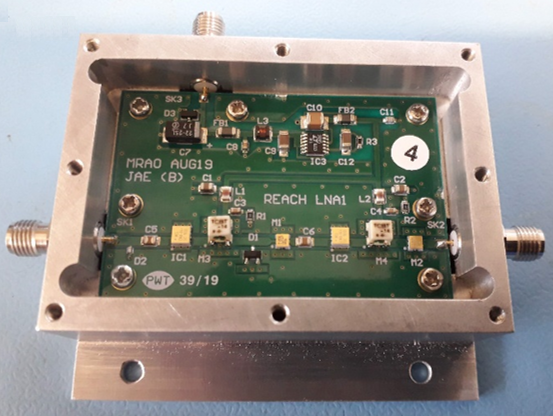
\includegraphics[scale=0.5]{lna}
    \caption{Interior of the completed REACH low noise amplifier custom designed for a flat spectral response in both S\textsubscript{11} and noise.}
    \label{fig:lna}
\end{figure}

While an alternative LNA built instead with Mini-Circuits ERA-50SM+ gain blocks exhibited a better noise figure of 3.3 dB, the CMA-84+ construction demonstrated a better stability in both S\textsubscript{11} and temperature. Reflection coefficients of the finalised LNA are plotted in \cref{fig:lna_sparams} showing the desired S\textsubscript{11} less than -30 dB which is well matched across the observational band as well as a remarkably flat 40 dB gain response.
\begin{figure}
    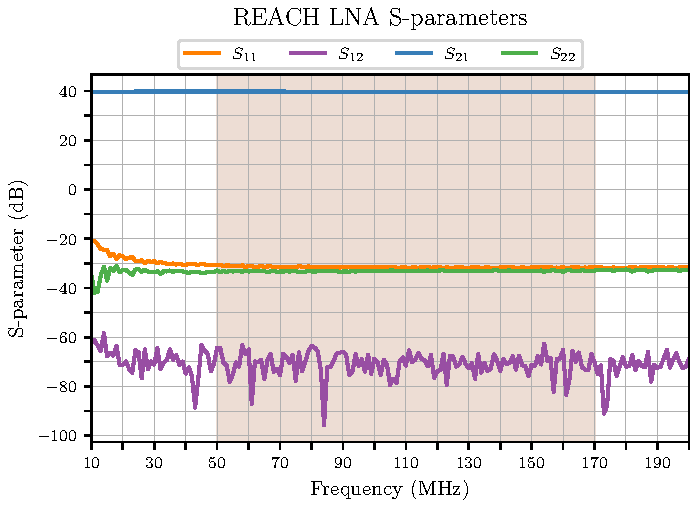
\includegraphics[width=\columnwidth]{lna_sparams}
    \caption{Measured S-parameters of the REACH LNA showing a good match at -30 dB for the $S_{11}$ and $S_{22}$ across the REACH observation band (shaded region) while demonstrating exceptional gain stability ($S_{21}$).}
    \label{fig:lna_sparams}
\end{figure}


% =========================================
\subsubsection{RF signal chain II: Amplifier \#1}
The second stage of spectral data amplification uses another custom module called ‘Amplifier \#1’, or AMP1\footnote{Like all good computer scientists, we have numbered our amplifiers using a zero-based system with the LNA, AMP1 and AMP2 being amplifiers number zero, one and two respectively in the RF signal chain.}. Incoming signals from the LNA are further amplified using a Mini-Circuits GALI-S66+ limiting amplifier and a PHA-13LN+ mid-power amplifier in combination to achieve maximal dynamic range followed by high-pass filtering using a Mini-Circuits RHP-44+ filter to attenuate frequencies below the observation band. A 2-stage Mini-Circuits XLF-42M+ monolithic microwave integrated circuit (MMIC) then low-pass filters out-of-band signals above the observation band up to many GHz.

Serving as the internal circuit boundary of the front-end receiver, AMP1 converts signals to Radio-Frequency-over-Fibre for transmission to the receiver back-end minimising the effects of RFI and signal loss that would be typical of alternative connections such as coaxial cables. The 1310 nm RFoF converter was made under commission by Polycom according to specifications for the HERA experiment. This passive module has approximately 18 dB of loss (measured S21) due to the relative intensity noise of the optical transmission laser.  Furthermore, there is a 1:2 ratio between optical loss and RF loss which needs to be accounted for in the link distances as presented in the field.

The total loss of the device would ordinarily impact the signal-to-noise ratio, however a large amount of upfront gain (up to 70dB) placed prior to the direct modulating laser, results in no impact on noise figure. These additional gain stages ensure the appropriate signal level is achieved at the ADC input after any losses over the RFoF conversion and link. The optical transmitter subassembly (as well as the corresponding back-end optical receiver) are printed circuit boards terminated in Fibre Channel/Angled Physical Contact (FC/APC) connectors at the end of a 0.5 metre pigtail as seen in \cref{fig:amp1}.
\begin{figure}
    \centering
    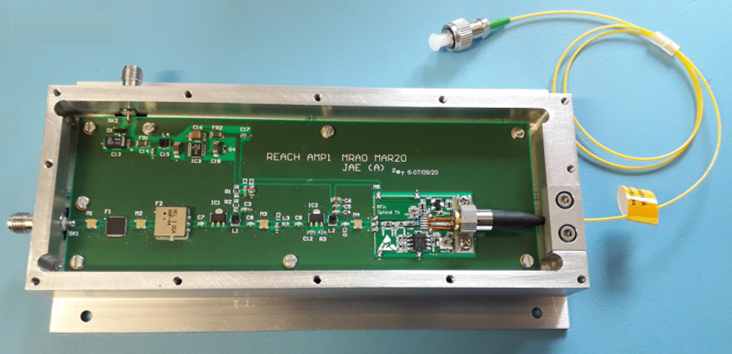
\includegraphics[scale=0.5]{amp1}
    \caption{The REACH AMP1 module used for further amplification and filtering of signals. Seen on the right end of the construction is the fibre optic conversion printed circuit board connected to the single-mode FC/APC RFoF transmission connector seen in yellow.}
    \label{fig:amp1}
\end{figure}
The FC/APC connector links to the RFoF port installed on the front-end enclosure as labelled in \cref{fig:enclosure_external_connections} which connects to an extended roll of fibre optical cabling reaching the receiver back-end. Single-mode fibre optics are again used to prevent signal degradation as with the USB-over-fibre connection. We find the radio-frequency loss of the RFoF bridge over the 100 metre distance to be less than 1 dB including the connections at both ends. A full circuit diagram of amplifier \#1 including the RFoF transducer is shown in \cref{fig:amp1_schematic}.


% =========================================
\subsubsection{Completed receiver front-end unit}
The deployable receiver front-end unit was completed in December 2022 and is shown in \cref{fig:frontend_complete}. 
\begin{figure}
    \centering
    \centering
    \begin{subfigure}{.45\textwidth}
        \centering
        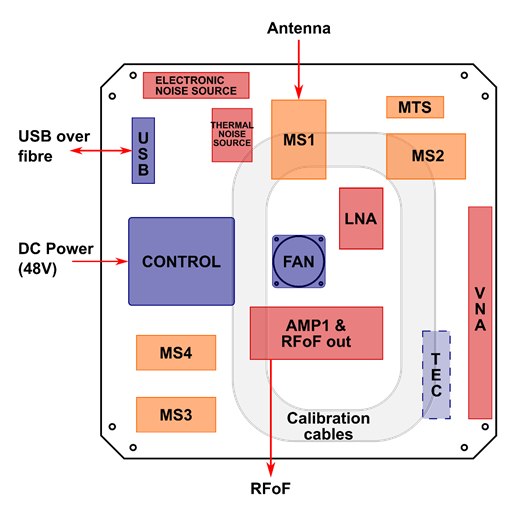
\includegraphics[width=\linewidth]{frontend_layout}
    \end{subfigure}
    \hfill
    \begin{subfigure}{.45\textwidth}
    \centering
        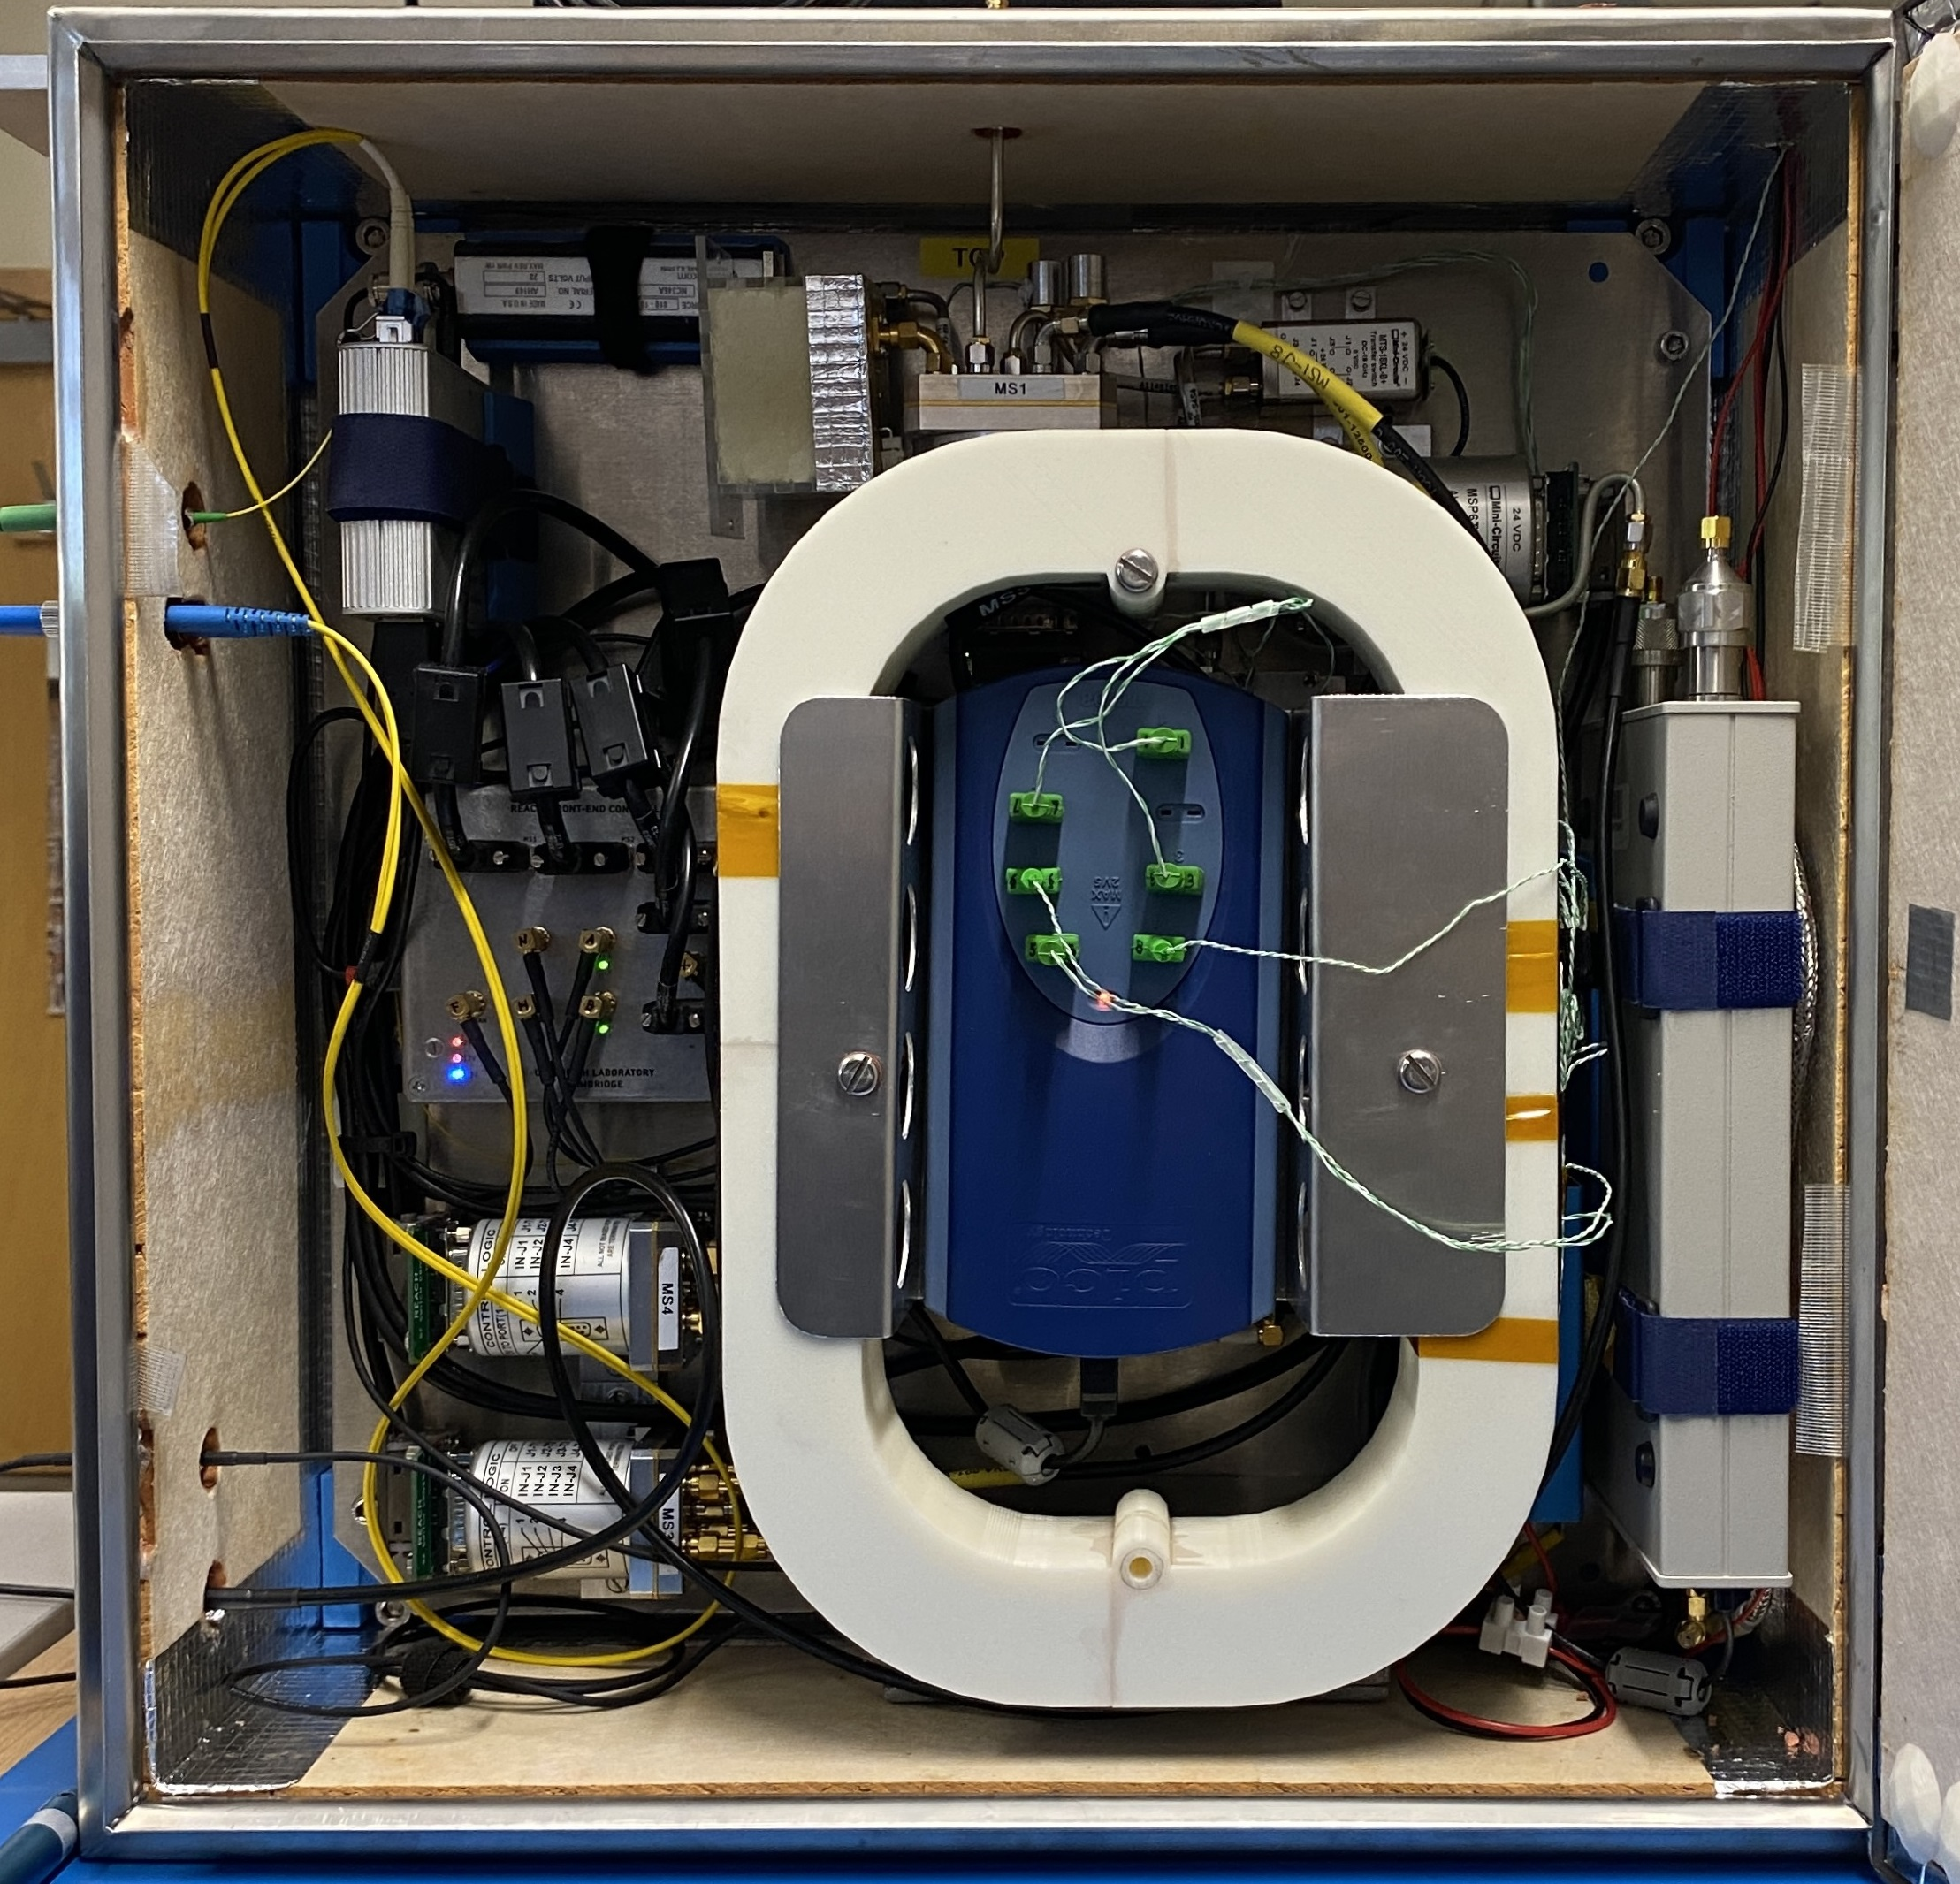
\includegraphics[width=\linewidth]{frontend.jpeg}
    \end{subfigure}
    \caption{The completed receiver front-end unit (right) along with a layout diagram showing the approximate positions of various components (left). Shown in the image are the compact VNA on the bottom right and the TC-08 module in the centre with green thermocouple probes. The stadium housing the calibration cables is seen around the TC-08 and obscures the amplifiers and TEC. The various cylinders are the multi-input switches connected to calibration sources. The microcontroller unit can be seen on the middle-left and is powered on as shown by the LED's. The USB over fibre link and diode noise source are shown in the top left corner. Layout diagram credit: Steven H. Carey.}
    \label{fig:frontend_complete}
\end{figure}
The finalised construction weighs 29 kilograms and, as stated previously, is allocated a maximum of 135 W for total front-end power from the solar panels. Control and RF circuitry require about 31.5 W with the remaining 103.5 W left for cooling through the TEC. The majority of the engineering work went in to construction of this receiver front-end and is expected to be deployed as a portable, energy efficient system with accurate in situ calibration through internal environmental control while maintaining the highest quality measurement capabilities and RFI mitigation. Also included are various ferrite beads to limit control and power signals from intercepting the RF signal path and were generally placed through trial-and-error. Subcomponents along the signal chain are connected with RG-402 semi-rigid cables to prevent cable flexing during transportation. A second 1:1 replica of the receiver is currently being built in Cambridge to assist in remote triage expected during deployment and design changes are being considered for future front-ends to accommodate additional antennas. A picture of the receiver front-end deployed on the REACH site in South Africa is shown in \cref{fig:frontend_deployed}.
\begin{figure}
    \centering
    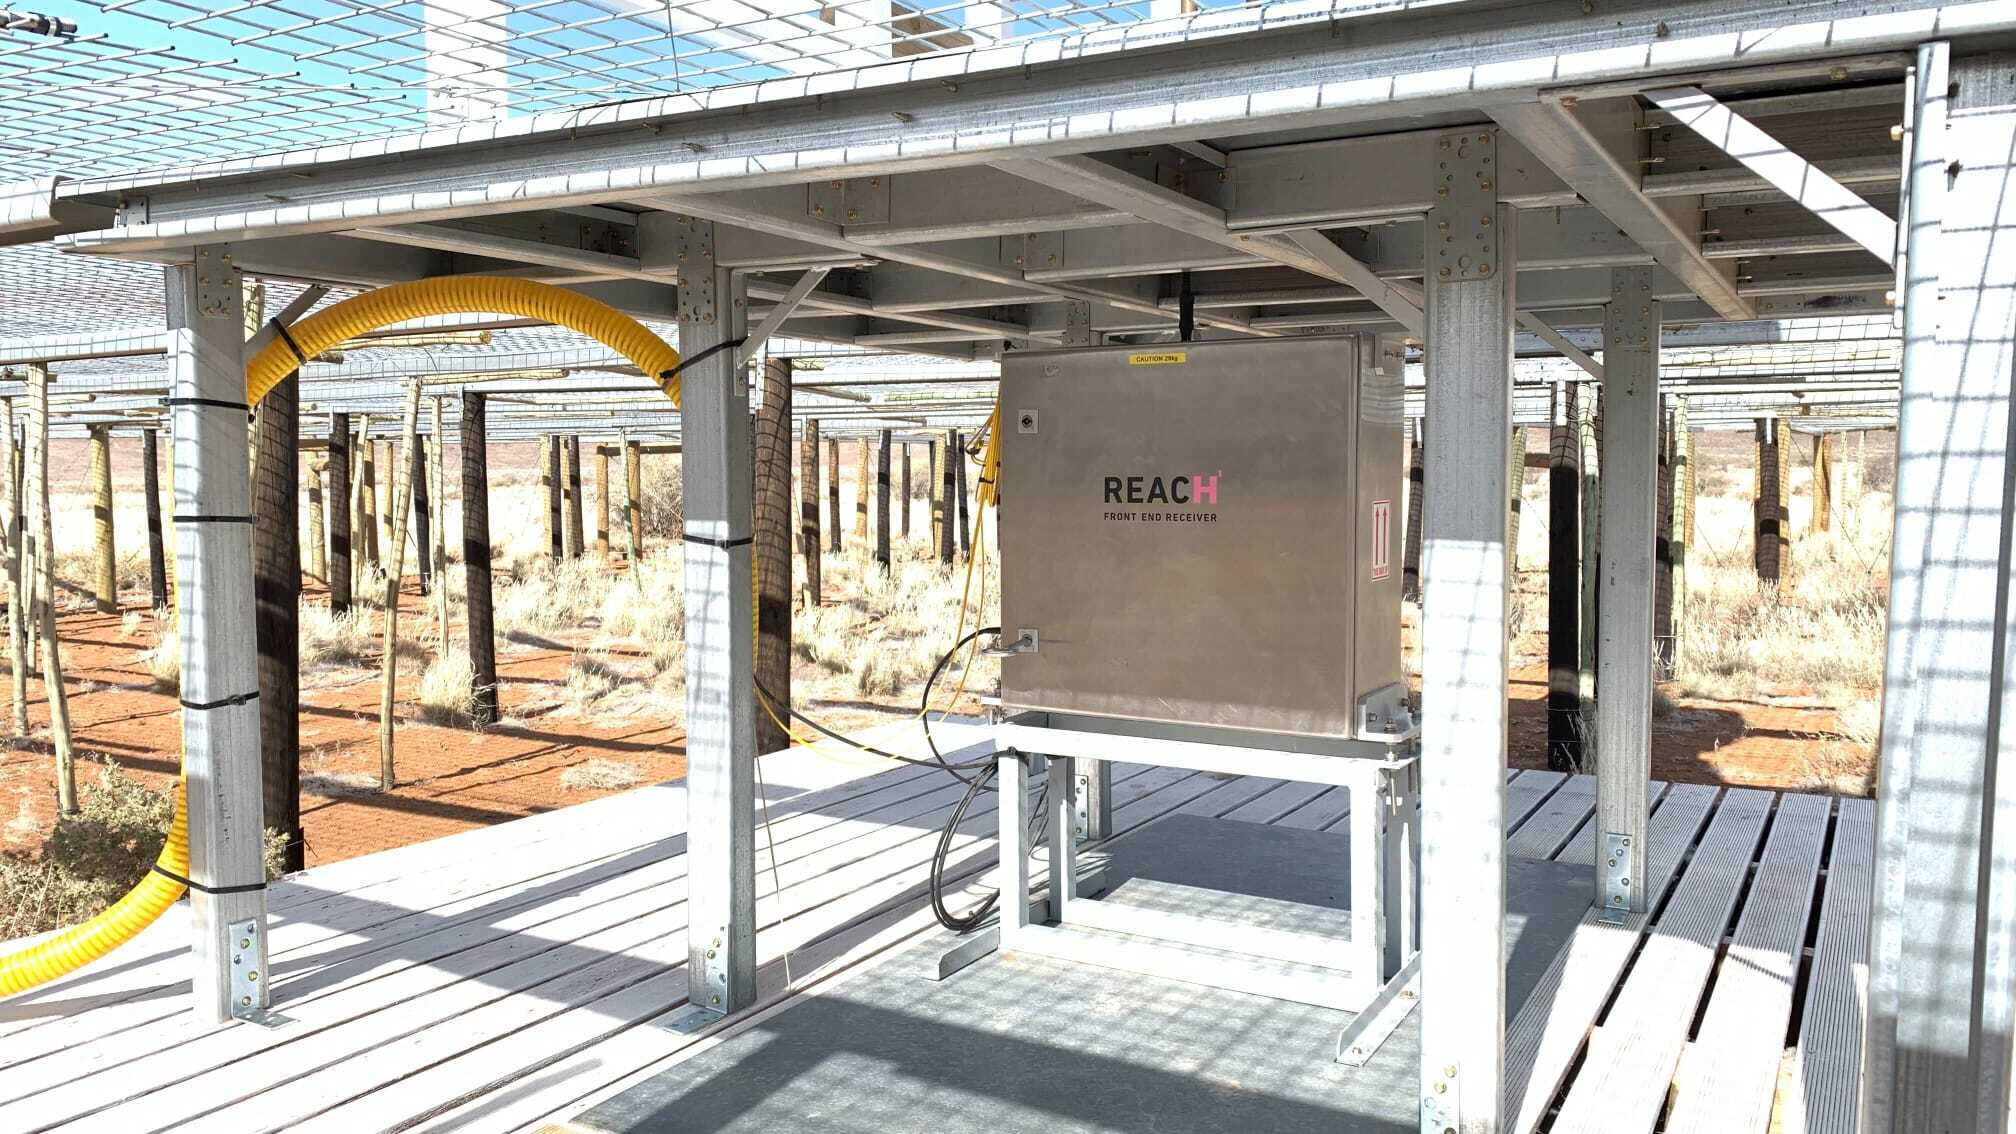
\includegraphics[width=0.8\textwidth]{receiver_installed.jpeg}
    \caption{The receiver front-end in its natural environment, deployed at the REACH experiment site in the Karoo Radio Astronomy Reserve, South Africa. Image credit: Dr. Saurabh Pegwal}
    \label{fig:frontend_deployed}
\end{figure}


% =========================================
\section{Receiver back-end}\label{sec:backend}
The receiver back-end houses the components critical for remote communication away from the deployment site, power distribution to the instrument as a whole and measurement subsystems that are less sensitive to environmental effects. 100 metres away from the dipole antenna, the receiver back-end sits below ten solar panels as diagrammed in \cref{fig:system_diagram}. This distance was chosen to avoid radio-frequency reflections off the solar panel and back-end faces as well as serving as a potential central node to be equidistant from future antennas. Under the solar panel construction is a radio-frequency electromagnetic-compatibility (RF-EMC) enclosure custom made by Interference Testing and Consultancy Services Ltd. to mitigate the effects of external RFI on our measurements as well as any potential EMI leakage from our own instrument that may be picked up by nearby experiments. Designs for the RF-EMC enclosure were informed by similar constructions used with the HERA experiment that incorporate considerations of the on-site environment as well as compliance with the EMC requirements of the Karoo Radio Astronomy Reserve. A conceptual diagram of the RF-EMC enclosure is shown in \cref{fig:backend}.
\begin{figure}
    \centering
    \centering
    \begin{subfigure}{.45\textwidth}
        \centering
        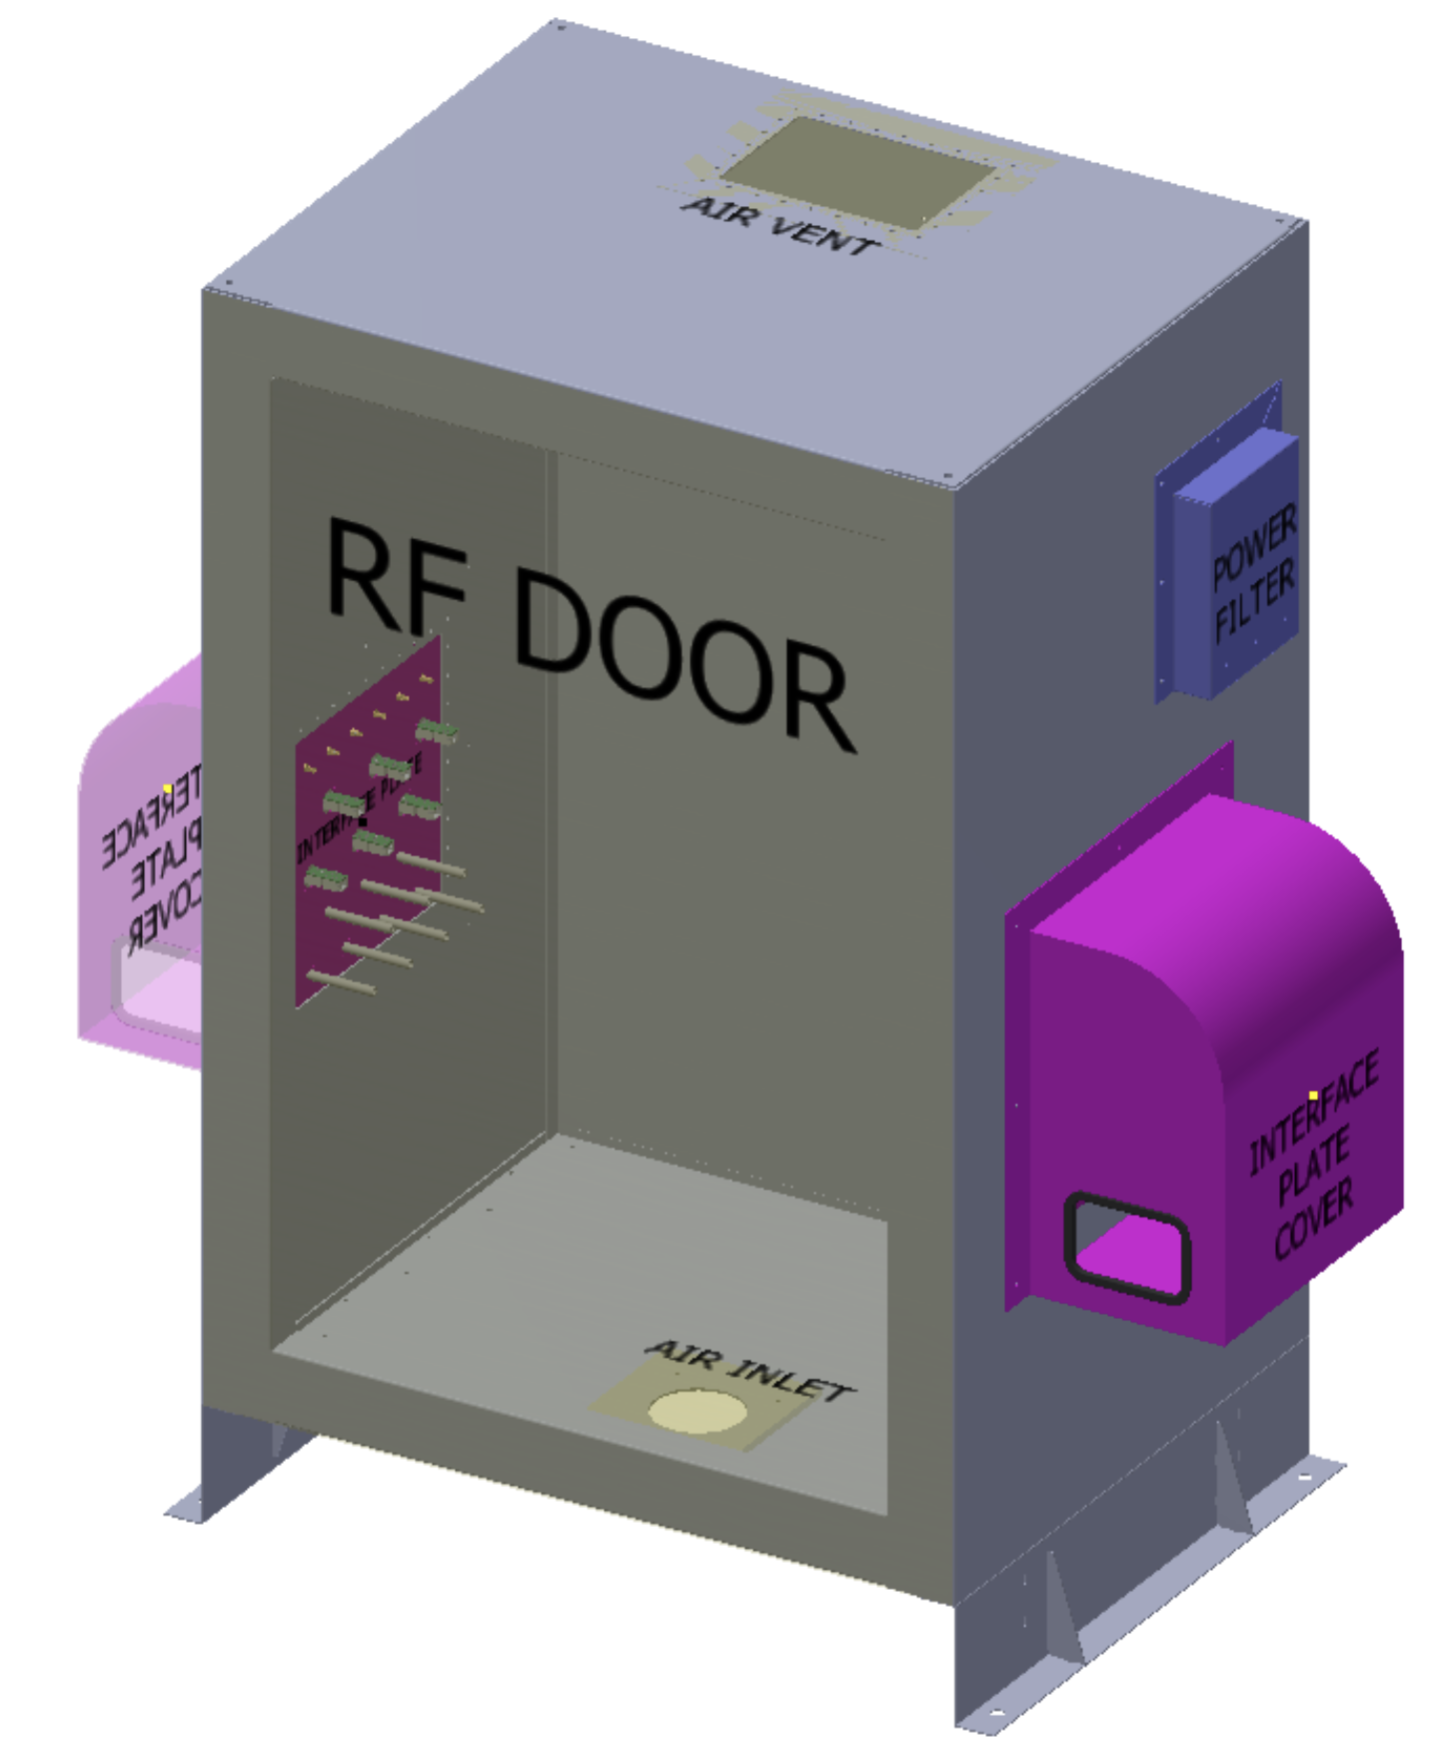
\includegraphics[width=\linewidth]{backend_diag}
    \end{subfigure}
    \hfill
    \begin{subfigure}{.4\textwidth}
    \centering
        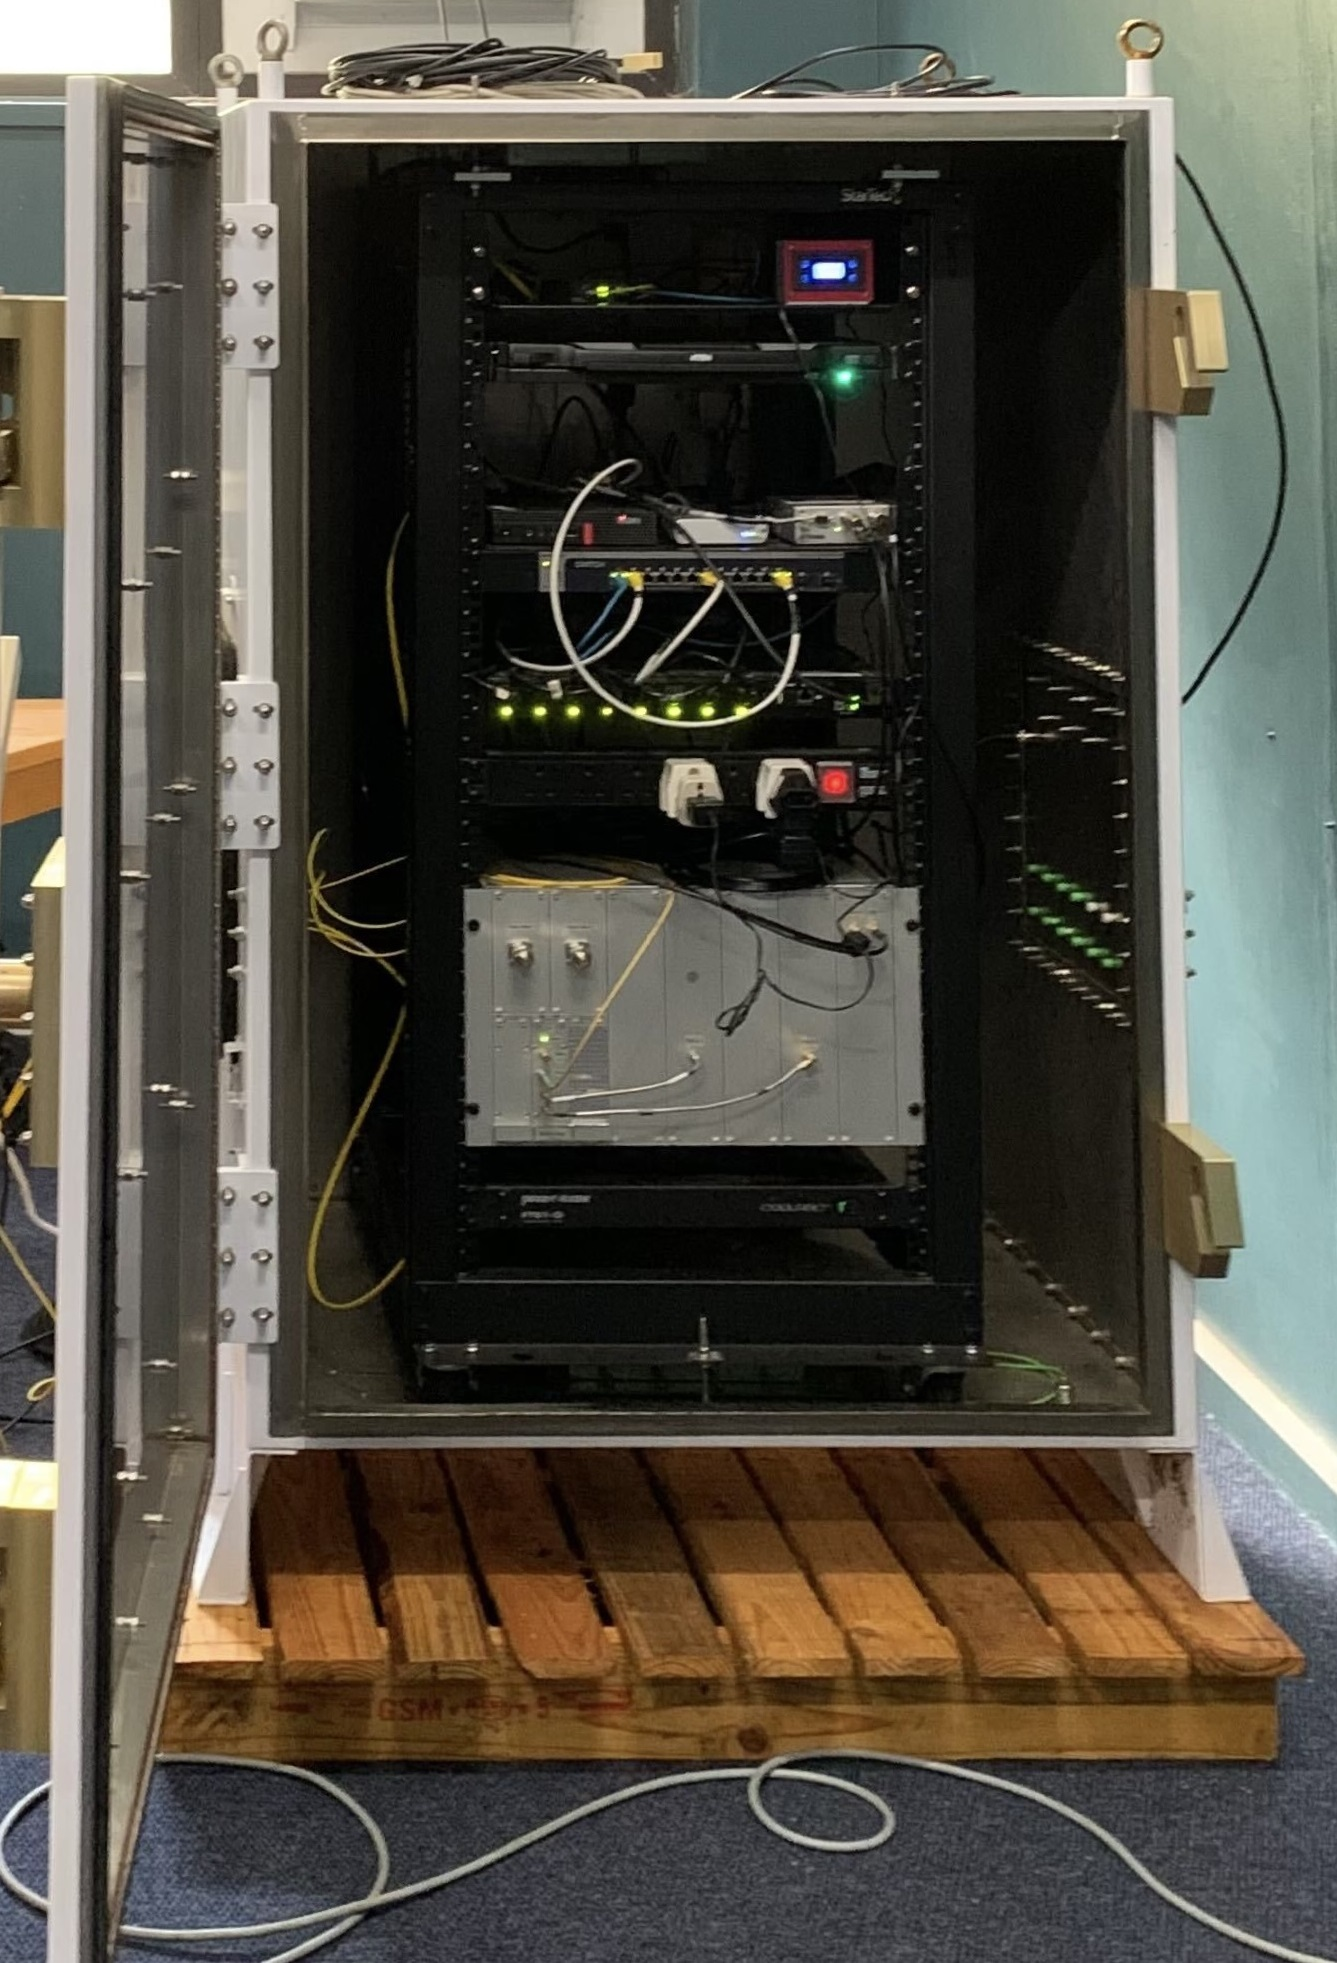
\includegraphics[width=\linewidth]{backend}
    \end{subfigure}
    \caption{A conceptual CAD rendering used as a reference for the REACH back-end RF-EMC enclosure is shown on the left exhibiting various custom assemblies for use in the South African Karoo such as ventilation paths and interference mitigation taken from \citet{hera_enclosure}. The right image shows the completed receiver back-end rack housed inside the RF-EMC enclosure. Rack components such as the amplifier and spectrometer assembly (large silver module), ventilation and power distribution units can be seen.}
    \label{fig:backend}
\end{figure}

Within the RF-EMC enclosure are the various back-end modules mounted on a 36-inch rack\footnote{A StarTech 22U 36 inch Depth Enclosed Server Cabinet was used in Cambridge but not shipped for deployment.} also shown in \cref{fig:backend} which includes modules for additional signal amplification, conditioning and digitisation, the spectrometer for measurement of power spectral data, the back-end server and GPS system for remote communication and automation of the device, as well as power distribution and cooling units as detailed in this section. The back-end RF-EMC enclosure is accompanied by a smaller similar chamber to house various additional units such as a 7400 Wh SS202 Lithium Iron Phosphate battery made by Solar MD for overnight power storage from the solar panels or during periods of non-ideal weather. This smaller chamber is shown in \cref{fig:power_chamber} for reference but is not strictly a part of the receiver back-end.


% =========================================
\subsubsection{RF signal chain III: Amplifier \#2 and out-of-band injection}
The first device in the receiver back-end is our third stage of amplification with Amplifier \#2 (AMP2). Upon entering AMP2, the RFoF signal from the front-end is converted back into an RF signal by the optical receiver, again constructed with an FC/APC connection to a Polycom printed circuit board mounted to the AMP2 module. The next task of AMP2 is to continue filtering the signal using another Mini-Circuits XLF-42M+ 2-stage MMIC low-pass filter to block high-frequency out-of-band signals. To sharply filter signals outside the REACH observational band (above 170 MHz), a custom 11-order Cauer Chebyshev low-pass filter was designed using a series of five 1812SMS air core inductors made by Coilcraft as shown in the circuit diagram \cref{fig:amp2_schematic}. Following this, the signal is amplified using two more Mini-Circuits GALI-S66+ and PHA-13LN+ amplifiers, as used in AMP1, to achieve best dynamic range prior to the analogue-to-digital converter (ADC) within the iTPM spectrometer module. Low-loss 3 dB Mini-Circuits RCAT-03+ equalisation circuits are also used throughout AMP2 to flatten the passband to 2 dB. The final sub-component of AMP2 is a power splitter to output two equal signals from the module with one path going to the ADC/spectrometer unit and the duplicated signal available for additional devices such as another ADC or a power meter for remote monitoring as done with the HERA experiment.

Supplementary to AMP2 was an optional module for out-of-band continuous wave or filtered noise signal injection to condition the ADC. This unit was built to inject a constant power (adjustable through the inclusion of attenuators) at 10 MHz and is band limited to DC--20 MHz, strictly outside the REACH observational band as not to contaminate the measurement. An example of the injected out-of-band noise from this module is shown in \cref{fig:oob_cond}, though this feature was not used in the final deployed system as it provided no tangible improvements to the data as discussed in the \cref{sec:responses}.
\begin{figure}
    \centering
    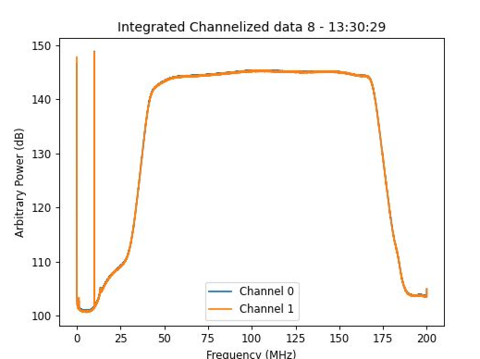
\includegraphics[scale=0.5]{oob_cond}
    \caption{A power spectral measurement of the ambient temperature $50 \Omega$ load with the out-of-band noise injection module activated. A constant power is injected at 10 MHz and can be used to assess the accuracy of the spectrometer reading as well as condition the ADC for low-power signals. Attenuators were used to prevent signals resonant to the 10 MHz injection from intercepting the in-band measurements. The spike at 0 MHz is an artefact of the spectrometer and receiver architecture and is not considered a hazard to the measurement.}
    \label{fig:oob_cond}
\end{figure}
The completed AMP2 and out-of-band injection unit are shown in \cref{fig:amp2} which represent the final components of the RF signal chain.
\begin{figure}
    \centering
    \includegraphics[scale=0.6]{amp2}
    \caption{The completed Amplifier \#2 (left) and out-of-band noise injection module (right) for inclusion in the receiver back-end. The ‘Fibre In’ port on AMP2 connects to the RFoF link from the front-end and the power splitter outputs identical signals to the ports labelled ‘Outputs’. The ‘Noise Output’ ports from the noise injection module would connect to the ‘Noise In’ port of AMP2 though this is not currently applied to measurements in the field.}
    \label{fig:amp2}
\end{figure}


% =========================================
\subsubsection{RF signal chain IV: Simulations}
Within the design process of the RF signal chain components; the LNA, AMP1 and AMP2, were various stages of optimisation and fine-tuning. Constituent elements within the LNA were first simulated then built and measured with the PNA-X as shown in \cref{fig:lna_sparams}. This data was then imported back into the simulation to further inform the development of the signal chain as a whole. Simulations were undertaken using the Keysight PathWave RF Synthesis software (formerly known as Genesys) with the in-program optimisation tool used to optimise filter design. Both linear analysis and the Keysight Spectrasys RF System Simulation software were also employed for RF budget simulations with other components simulated using Modelithics’ substrate scalable models. Also included in the simulations were measurements the AMP1 optical transmitter, AMP2 optical receiver and 100 metres of single-mode fibre, characterised by the VNA at different power levels and added to the simulation as a single block as shown in \cref{fig:chain_block_diag} which replicates the complete RF signal chain.
\begin{figure}
    \centering
    \includegraphics[width=\textwidth]{chain_block_diag}
    \caption{REACH RF system end-to-end block simulations made with the Keysight PathWave RF Synthesis software showing the LNA, AMP1, AMP2 as well as the RFoF link.}
    \label{fig:chain_block_diag}
\end{figure}
The results of the full RF signal chain simulations are shown in \cref{fig:chain_sim} where we highlight the flat noise figure of the network over the observational band.
\begin{figure}
    \centering
    \includegraphics{chain_sim}
    \caption{Simulated radio-frequency response of the REACH end-to-end signal-chain as diagrammed in \cref{fig:chain_block_diag} which includes the LNA, AMP1, AMP2 and RFoF modules. VNA measurements of the LNA have been included in this simulation as well. The shaded region represents the REACH observation band where we see a flat noise figure throughout. Adapted from figure included in \citet{reach}.}
    \label{fig:chain_sim}
\end{figure}


% =========================================
\subsubsection{Spectrometer}
Following the amplification stages is the Sanitas EG \textit{italian} Tile Processor Module (iTPM) shown in \cref{fig:tpm} which serves as an analogue-to-digital converter (ADC) and a high-resolution ultra-wideband digital spectrometer.
\begin{figure}
    \centering
    \includegraphics[scale=0.4]{tpm}
    \caption{The Sanitas EG italian Tile Processor Module for conversion of analogue signals to digital as well as spectral measurements. Image taken from Sanitas EG website: \url{https://www.sanitaseg.com/project/itpm-adfe/}.}
    \label{fig:tpm}
\end{figure}
This device was chosen for its development under the Square Kilometre Array experiment as part of the Low Frequency Aperture Array and has been used for verification of an SKA1 station as well as for back-end signal processing in other experiments \citep{itpm}. The iTPM's design targeting similar EoR signals granted easy reconfiguration for the REACH experiment through the reuse of auxiliary functions such as control, monitoring and data acquisition. Conversion of the incoming analogue signal to digital is undertaken using sixteen dual-channel Analog Devices 14-bit AD9680 ADCs allowing for multiple data streams from additional proposed antennas as detailed in \cref{sec:future}. At the time of deployment, two ADC channels were initialised as seen in the \cref{fig:oob_cond} legend for the two antennas expected to be built with the remaining ADC channels disabled to save power. Analogue signals are digitised at 400 MSPS using 16,384 channels at 12.2 kHz per channel. After conversion, spectral measurements are taken by two AMD XILINX UltraScale XCU40 field-programmable gate arrays (FPGAs) each customised to process a single digitised RF signal using a full floating-point fast Fourier transform (FFT), power integrator and polyphase filter bank incorporating 229,376 tap coefficients downloadable to the FPGA to allow the implementation of different weighting functions without recompiling the FPGA firmware. Spectra are accumulated over a number of FFT frames corresponding to an integration time of approximately one second which are then transmitted to a processing server via Ethernet connection where further accumulation can take place on the order of minutes. A typical spectrum obtained from a 20-minute integration on the $50 \Omega$ cold load is shown in \cref{fig:psd_cold}.
\begin{figure}
    \centering
    \includegraphics{psd_cold}
    \caption{A spectra taken by the iTPM of the ambient temperature $50 \Omega$ load integrated for 20 minutes using the finalised receiver system. A stable power measurement is seen within the REACH observational band (shaded region).}
    \label{fig:psd_cold}
\end{figure}
The >90 dB channel isolation of the spectrometer is expected to be useful for RFI excision \citep{itpm}. While on-site RFI measurements are still needed to confirm this, data from co-located experiments such as HERA suggest that the current channel isolation is adequate \citep{hera}.


% =========================================
\subsubsection{Readout enclosure}
The readout system comprised of AMP2, the digitiser and spectrometer is housed in a custom-built 6U\footnote{housing height of six standard rack units approximately equal to 266.7 mm} metal enclosure as shown in \cref{fig:readout_enclosure}.
\begin{figure}
    \centering
    \includegraphics[width=0.7\textwidth]{readout_enclosure.jpeg}
    \caption{The readout enclosure housing the receiver components needed for digitisation and spectral measurements of radio-frequency signals.}
    \label{fig:readout_enclosure}
\end{figure}
Included in the readout enclosure are installations for two USB power meters to independently monitor absolute power levels in the field as previously detailed as well as slots for the out-of-band noise injection module and two independent Amplifier \#2 modules to accommodate two antennas in the field. Semi-rigid RG-405 connect the AMP2 outputs to iTPM channel inputs allocated individual panels seen in \cref{fig:readout_enclosure}. Within the enclosure is an off-the-shelf Peltier heat exchanger, fan and insulation to help regulate the temperature of the readout system, though the back-end components are subject to less scrutiny for operating temperature and output directly to the communication server via RJ45 cabling. Also seen on the front panelling are timing inputs to connect the iTPM to the GPS unit as detailed in the next subsection.


% =========================================
\subsubsection{GPS unit for TPM synchronisation}
Tile processor modules, such as the one used in our readout system, are comprised of a series of processing units referred to as ‘tiles’ which work in tandem to perform tasks efficiently. For precision applications, synchronisation among tiles is crucial for overall performance and a reference oscillator is needed to provide a common clock signal coordinating the timing of operations across different tiles. As we do not know the environmental effects of the deployment site on the iTPM’s internal oscillator a priori, we use an external Thunderbolt E GPS disciplined clock made by Trimble to ensure iTPM tiles operate in harmony. The Thunderbolt E links to a proprietary GPS antenna through a $75 \Omega$ Belden 1189A cable which allows the module to communicate with the global positioning system to generate a 10 MHz oscillation which is used as a reference to produce a 400 MHz clock to set the ADC sampling rate of 400 MSPS. The module then relays a pulse per second (PPS) signal to synchronise the ADCs to ensure coherence. The GPS disciplined clock was chosen over alternative atom-based frequency standardisation modules to ensure the reference clock accuracy, and in turn the sampling clock accuracy, is isolated from environmental effects, damage during transport, or interference generated by our own receiver components. This would in theory increase accuracy by limiting the propagation of delayed clock signals across tiles (known as skewing), and small variations in clock signal timings (known as jitter). Furthermore, a single reference should be used when using multiple TPMs, as may be the case in the future, to avoid slightly different sampling rates based on individual oscillators. Users of the receiver back-end should note that the 10 MHz GPS signal is independent from the 10 MHz out-of-band noise injection and are urged to be aware of the similarly-named labelling throughout the instrument. The Trimble Thunderbolt E as well as its GPS antenna are shown in \cref{fig:gps}.
\begin{figure}
    \centering
    \centering
    \begin{subfigure}{.3\textwidth}
        \centering
        \includegraphics[width=\linewidth]{trimble}
    \end{subfigure}
    \hspace{.15\textwidth}
    \begin{subfigure}{.33\textwidth}
    \centering
        \includegraphics[width=\linewidth]{gps_ant}
    \end{subfigure}
    \caption{The Trimble clock discipline system consisting of the Thunderbolt E reference signal generator (left) and GPS antenna (right). Left image taken from novotech website: \url{https://preview.novotech.com/thunderbolt-e-gps-disciplined-clock-304.html}.}
    \label{fig:gps}
\end{figure}


% =========================================
\subsubsection{Server \& additional back-end units}
To permit communication between the instrument and users at Cambridge, a Lenovo M920q Tiny ThinkCentre with a ninth generation Intel i7 core is included in the receiver back-end as a server. Xubuntu was chosen as the server operating system as the Xfce desktop environment uses fewer system resources in the field while retaining the flexibility and ease of use of Ubuntu\footnote{sorry Arch users…}. The ThinkCentre’s visual output connects to an ATEN CL6700 MW Single Rail LCD Console with built-in monitor keyboard and trackpad\footnote{Also referred to as a ‘KVM’ console for ‘Keyboard, Video \& Mouse’.} for in-person interaction with the machine during installation, triage and site trips when network connection may not be available.

USB links between the server and receiver components is achieved with a StarTech 10-port USB hub with its primary function of receiving the USB over fibre signal from the front-end through the Icron 2244 USB Ranger’s optical-to-USB transducer. As detailed in \cref{sec:frontend}, this allows for the collection of reflection coefficient and temperature data as well as transmission of instructions to the microcontroller and front-end thermal management system. Additional ports on the StarTech USB hub connect the server to the back-end TEC controller for the Peltier device within the readout enclosure as well as a Penn Elcom FT01-Q module consisting of three rack-mounted fans for airflow and cooling within the receiver back-end. Finally, the USB hub connects the server to a Netgear ProSafe M4100-D12G Ethernet managed switch for control of further components via RJ45 connection. Connected to the Ethernet switch is the readout system output, permitting the collection of spectral data from the iTPM as well as connection to a Tripp Lite PDUMH15HVNET Ethernet controlled power distribution unit allowing users to toggle power for individual devices throughout the receiver back-end. The Ethernet switch will also be connected to the satellite uplink intended to be installed after the receiver back-end but not finalised at the time of writing. A second PDU was included in the deployed back-end but is not used. Tables specifying the connections of the USB hub, Ethernet switch and back-end PDU are given in \cref{tab:usb_hub}, \cref{tab:eth_switch} and \cref{tab:backend_pdu} respectively for reference.


% =========================================
\subsubsection{Completed receiver back-end unit}
The receiver back-end was also finished in December 2022 and is shown in \cref{fig:backend_complete}.
\begin{figure}
    \centering
    \includegraphics[width=.7\textwidth]{backend_complete}
    \caption{The completed receiver back-end installed in the 36-inch rack in Cambridge (minus the RF-EMC enclosure). The custom readout system weighs in at 15.89 kilograms and is central to the experiment's data acquisition. The Ethernet switch and power distribution units can be seen and are controlled by the Lenovo server. This unit would be common to any additional antennas deployed to the field and is generally less sensitive to environmental effects on site.}
    \label{fig:backend_complete}
\end{figure}
The completed build was too large to be shipped practically and was disassembled into its constituent submodules before being sent to South Africa in February 2023 and reconstructed using a different standardised rack. This finalised construction is intended to serve as a central node for the REACH experiment including any further antennas to be deployed on site. As much of the receiver back-end consists of off-the-shelf components, we expect serviceability and part replacement to be more straightforward than the front-end. A diagram indicating the back-end submodules is shown in \cref{fig:backend_diag}.
\begin{figure}
    \centering
    \includegraphics[width=\textwidth]{backend_components}
    \caption{A diagram specifying the placement of the various back-end components for the completed unit in December 2023.}
    \label{fig:backend_diag}
\end{figure}


% =========================================
\section{Automation}
The nearest settlement to the REACH deployment site in the Karoo Radio Reserve is Carnarvon, about 90 kilometres away and about seven hour’s drive from the central international airport in Cape Town. Such isolation made the development of a fully autonomous instrument a necessity and procedures were developed to facilitate remote access and communication with the device. In our procedure, the receiver front-end(s) and back-end are controlled and monitored by our management software running on the Lenovo processing server which oversees operation of the instrument such as the configuration of hardware components, data management and directing subroutines. Within our management software, a variety of different communication protocols are used. The Python FPGA Board Interface Layer (PyFABIL) is used to interact with the iTPM while the Standard Commands for Programmable Instruments (SCPI) protocol is used to contact the VNA. Proprietary USB protocols in a Python wrapper are used by the TC-08 temperature sensor with the TEC needing an additional proprietary Windows-based Application Programming Interface which entails a virtual machine running in our Linux desktop environment. Signal path configuration through the microcontroller unit is assigned to Teensy ports accessed through a command line serial interface. A crib sheet useful for the development of automated procedures such as an observation schedule is shown in \cref{fig:controller_pinout} which details the specific devices contactable through individual microcontroller ports.
\begin{figure}
    \centering
    \includegraphics{controller_pinout}
    \caption{A reference sheet listing the front-end component assignments to the Teensy input/output ports for use in receiver automation. Individual switch positions, power supplies and components can be seen facilitating the creation of new automated routines and on-the-fly system interaction via command line interface. MS‘N’--‘P’ refers to mechanical RF switch number N, port P. ‘MTS’ is the mechanical transfer switch. ‘TEC’ is the thermoelectric cooler module. Image credit: Steven H. Carey.}
    \label{fig:controller_pinout}
\end{figure}

Both the calibration and observation procedures are managed by a YAML configured scheduler allowing a remote operator to specify a sequential list of operations including switch toggling, reflection coefficient or spectral measurement, the VNA calibration and hardware initialisation among other low-level commands for debugging purposes. General prescriptions are provided for the two main operations, the first of which is calibration. During calibration, the instrument is instructed to first calibrate the VNA through measurement of the S-O-L standards as detailed in \cref{sec:frontend}. Following this, a measurement of the $50 \Omega$ test load is compared to a saved file from the PNA-X on a frequency-by-frequency basis. If the VNA measurements are within a user-defined tolerance (usually 5\%), the instrument proceeds with receiver calibration measurements; S\textsubscript{11}, spectra and temperatures of the calibration sources along with an S\textsubscript{11} measurement of the LNA. This data is fed into the calibration algorithm to generate calibration coefficients which are verified through comparison with a benchmark set of coefficients to within a user-defined tolerance (e.g. previous calibration coefficients to within 5\%).

Following this is the second primary mode of operation; observation. During observation, power spectral measurements of the sky, reference load and reference noise source as part of the Dicke cycle are performed by the YAML-configured schedule started by a local sidereal time (LST) trigger. Additional measurements of the test load are taken to support ad hoc debugging procedures after which RFI in the data is flagged by a separate algorithm. Calibration coefficients derived in the calibration routine are then applied to the data before being set for data processing. A flowchart depicting the general steps of instrument operation is shown in \cref{fig:obs_flowchart}.
\begin{figure}
    \centering
    \includegraphics[width=\columnwidth]{updated_reach_obs_loop}
    \caption{Typical REACH calibration and observation loop including calibration of the VNA and receiver as well as data acquisition, checks and processing such as RFI flagging. Various stages are verified via algorithm before proceeding to the next process.}
    \label{fig:obs_flowchart}
\end{figure}

The receiver back-end transmits integrated spectra as Streaming Protocol for Exchanging Astronomical Data User Datagram Protocol (SPEAD UDP) packets over a 1 GbE network to be received by the associated spectrometer module. A software monitoring daemon collects temperature and power information every minute which is stored in a metric database which are included as metadata with calibration and observation data to inform the calibration procedure. The generated data is then stored as an HDF5 file which includes spectra and reflection coefficients with associated timestamps along with temperature sensor readings. The HDF5 files are self-describing, containing all the information required for future processing without having to refer to observation schedules or similar documentation. The HDF5 files then are transferred off-site to a centralised storage system through a satellite network link installed on-site. An plot of power spectral data taken remotely from Stellenbosch University in South Africa is shown in \cref{fig:remote_data}.
\begin{figure}
    \centering
    \includegraphics[scale=0.6]{remote_data}
    \caption{Passband measurements of several calibration sources taken remotely through an automated procedure showing a clean frequency response. Image credit: Prof. Alessio Magro.}
    \label{fig:remote_data}
\end{figure}


% =========================================
\section{Deployment}
Throughout 2022, the deployment site in South Africa was prepared while receiver development took place. Ditches were dug for support posts to be placed for the raised ground plane mesh suspended by guide wires. Due to natural land slope on site, the ground plane was erected between 1 metre and 1.2 metres above ground level to maintain a level construction. Support structures were built and the antenna was then installed as shown in \cref{fig:ground_plane}.
\begin{figure}
    \centering
    \includegraphics[width=\textwidth]{ground_plane}
    \caption{The REACH dipole antenna on the raised wire mesh ground plane. Support posts of heights varying 20 cm were raised to provide a level ground plane in contrast to the sloped land underneath.}
    \label{fig:ground_plane}
\end{figure}
Upon being shipped from Cambridge, the receiver front and back-ends underwent strict electromagnetic compatibility (EMC) testing at the Karoo radio reserve under the same level of scrutiny as co-located experiments such as HERA. After a final round of testing by the REACH team, the receiver was transported to the deployment site in August 2023 where the back-end components were installed as shown in \cref{fig:deploy_backend}.
\begin{figure}
    \centering
    \includegraphics[width=.8\textwidth]{deploy_backend.jpg}
    \caption{The receiver back-end and support enclosure underneath the solar panel installation at the deployment site. Image credit: Dr. Saurabh Pegwal.}
    \label{fig:deploy_backend}
\end{figure}

It was understood that at some time between shipment from Cambridge and deployment in the field that both the front-end TEC Peltier device as well as satellite infrastructure had been damaged and no longer functioned. The front-end has been sent back to Stellenbosch University to investigate the fault. Despite this, in-field sky spectra was taken, a screenshot of which can be seen in \cref{fig:onsite_data}.
\begin{figure}
    \centering
    \includegraphics[scale=0.4]{onsite_data}
    \caption{A screenshot from the REACH's first light showing on-site sky data collected by the dipole and taken directly from the back-end KVM console using a mobile phone. The themo-electric cooling unit damaged during transport was not running during this data acquisition. The spectra seen are uncalibrated and underwent no data processing which causes the spectra to deviate from the characteristic power-law form expected of the foregrounds at low and high frequencies. The shaded region is the FM radio broadcast band for South Africa (87.5 -- 108 MHz).}
    \label{fig:onsite_data}
\end{figure}
As a disclosure, it should be noted that this in-field data was left on a USB flash drive on site and here, a snapshot from the KVM screen taken with a phone camera is used. The image has been enhanced using Microsoft Lens and the GNU Image Manipulation Program (GIMP). While the spectra shown in \cref{fig:onsite_data} is raw, uncalibrated data that hasn't gone through any processing, some important details can be derived from the plot. Firstly, spectra from the antenna is generally higher than the calibrator spectra which serves as a sanity check. Secondly, more than half of the RFI spikes seen in the antenna spectra lie within the FM radio broadcast band for South Africa (87.5--108 MHz) as highlighted in purple, confirming that our apparatus is indeed receiving radio-frequency signals. Further verification can be undertaken by cross checking the precise broadcast frequencies of local radio stations. Finally, we can also see that the antenna spectra peaks at low frequencies and decays off, approximating the power law shape of galactic synchrotron emission expected from sky measurements at these frequencies (compare with Figure 1a of \citet{edgesNature}). We therefore conclude that these spectra are encouraging as an initial proof-of-concept measurement.

Furthermore, it has also been seen that, due to the changing weather conditions on site, the $20 \times 20$ metre ground plane\footnote{with 6 metre serrations} sags due to insufficient support. Provisional supports were made with scrap wood as seen in \cref{fig:ground_plane} while a more permanent method of support is currently deployed. With the approximate completion of the ground plane, installation of the dipole antenna, solar panels and receiver back-end, the REACH site can be seen through satellite imaging at the latitude-longitude coordinates 30\textdegree50'19.4"S 21\textdegree22'29.8"E as shown in \cref{fig:sat_image}.
\begin{figure}
    \centering
    \includegraphics[width=\textwidth]{sat_image}
    \caption{A satellite image from Google Earth showing the REACH deployment site. The 20 metre wide ground plane can be seen with the antenna installed at its centre. To the upper right of the ground plane is the back-end node covered by the solar panel installation. The lower left shows two vehicles and a tent with a dirt road exiting the site on the left along the ground plane. Image taken from Google Earth.}
    \label{fig:sat_image}
\end{figure}

\chapter{Receiver calibration}\label{chap:calibration}

% **************************** Define Graphics Path **************************
\ifpdf
    \graphicspath{{calibration/figs/Raster/}{calibration/figs/PDF/}{calibration/figs/}}
\else
    \graphicspath{{calibration/figs/Vector/}{calibration/figs/}}
\fi


With a working instrument capable of taking measurements in the field, the next step towards detection of the 21-cm signature is calibration of the experimental apparatus. There are many forms of calibration from physical antenna or ground plane modifications to numerical post-processing methods such as correctional atmospheric modelling. The need for more accurate cosmic signal measurements against the cacophony of unwanted noise demands finer degrees of calibration through the development of novel methods. At the current technological aim of millikelvin-level calibration, minute differences in an instrument’s electrical properties can skew spectral measurements enough to hamper a cosmological detection. In the previous chapter, we detailed the system architecture designed to minimise these distortions. Here we present a procedure to calibrate out the remaining systematic effects. The task has encompassed decades of research starting in the 1950’s where \citet{bauer_rothe} and \citet{rothe_dahlke} introduced a wave formulation of noise to microwave systems\footnote{\citet{bauer_rothe} presented in English by \citet{penfield}.} before a mathematical prescription to eliminate these noise waves through the derivation of “noise wave parameters” was conceived by \citet{meys} in 1978. This method, which inspires many contemporary radiometric calibration procedures, relies on the relative differences between sequential measurements of known passive devices to divide out small-timescale variability through a method known as “Dicke switching”, named after famed astronomer Robert Dicke. This relative calibration was utilised into the late 2000’s when \citet{edges_limits} placed a lower limit on the duration of the reionisation epoch at $\Delta z < 0.06$.

It was quickly understood that the extraction of further information from 21-cm experimentation required a more powerful calibration method and work commenced to reformulate the noise wave parameters under an “absolute” calibration procedure which offered a more comprehensive derivation by referencing all measurements to an absolute temperature scale as well as expanding compatibility with instruments of increasing bandwidth \citep{rogersCal}. It was this absolute calibration that was used in the 2018 EDGES measurement where the authors quote a 20 mK calibration accuracy \citep{edgesNature, edgesCal}. In response to the controversy surrounding the EDGES experiment, we have strived to improve the methodology and address discrepancies in the procedure through the introduction of a Bayesian calibration framework which we formulate over the following sections.


% =========================================
\section{Calibration formalism}\label{sec:formalism}
The noise necessitating calibration arises during measurements. For a global experiment such as REACH, we measure a sky temperature $\T{sky}(\Omega, \nu, t)$ as a function of the direction $\Omega$, frequency $\nu$ and time $t$ which can be broken down into two primary components: the global 21-cm signal $T_{21}$ and astrophysical foregrounds $\T{f}$
\begin{equation}
    \label{tsky}
    \T{sky}(\Omega, \nu, t) = T_{21}(\nu) + \T{f}(\Omega, \nu, t).
\end{equation}
Sky signals absorbed by the antenna convolve with the normalised antenna directivity $B$ ,introducing systematic noise represented by our random noise term $N_{\mathrm{data}}$.
\begin{equation}\label{eqn:bayestsource}
    D(\nu, t) = \int \T{sky}(\Omega, \nu, t) B(\Omega, \nu)\mathrm{d}\Omega + N_{\mathrm{data}}.
\end{equation}
Thus, our 21-cm signature can be formulated as
\begin{equation}\label{signal}
  T_{21} \approx D(\nu, t) - \int\T{f}(\Omega, \nu, t)B(\Omega, \nu)\mathrm{d}\Omega - N_{\mathrm{data}}.
\end{equation}
A diagram illustrating the evolution of the sky signal during this process in shown in \cref{fig:nsfig}.
\begin{figure}
    \centering
    \includegraphics[width=.7\textwidth]{nsdiag}
    \caption{Diagram showing the evolution of the 21-cm signal hampered by astrophysical foregrounds, convolvution with the antenna beam and the emergence of measurement noise before calibration to retrieve the sky temperature.}
    \label{fig:nsfig}
\end{figure}
The integral in \cref{signal} is assessed through foreground and beam modelling techniques such as those discussed in \citet{dom} while modelling of $N_{\mathrm{data}}$ from the (statistical) properties of $D(\nu, t)$ is accomplished through calibration.

The standard calibration strategy follows the method introduced by Dicke to characterise systematic features in radio-frequency instruments \citep{dickeplus} and is widely used in experiments such as EDGES \citep{edgesCal} and LOFAR \citep{lofarCal} to evaluate the spectral index of the sky's diffuse radio background \citep{rogersCal}. The technique involves measurements of two internal reference standards; a load and a noise source, in addition to a series of external calibration sources attached to the receiver input in lieu of the antenna. Historically these include an ambient-temperature ‘cold’ load, a ‘hot’ load heated to $\sim 400$ K, an open-ended cable and a shorted cable as detailed previously in \cref{fig:dicke}.

During a calibration measurement, power spectral densities (PSDs) are taken of each Dicke switch position; the receiver input ($\psd{cal}$), the internal reference load ($\psd{L}$) and the internal reference noise source ($\psd{NS}$) \citep{edgesCal}. These measurements are used to calculate a preliminary `uncalibrated' antenna temperature $\T{cal}^*$
\begin{equation}
  \label{eqn:tantstar}
  \T{cal}^* = \T{NS} \left(\frac{\psd{cal}-\psd{L}}{\psd{NS}-\psd{L}}\right) + \T{L},
\end{equation}
where $\T{L}$ and $\T{NS}$ are assumptions for the noise temperature of the internal reference load and excess noise temperature of the internal noise source above ambient, respectively. This comparison of sequential power measurements serves as the `relative' calibration which removes time-dependent variations in system gain emerging from individual components or technical capabilities of the instrument \citep{edgesCal}. These PSD measurements can be expanded in terms of specific response contributions with the input power spectra being
\begin{multline}
  \label{eqn:pant}
  \psd{cal} = g_{\mathrm{sys}} \Bigg[ \T{cal}\left(1-|\Ga|^2\right)\left|\frac{\sqrt{1 - |\Gam{rec}|^2}}{1-\Ga\Gam{rec}}\right|^2 + \T{unc}|\Ga|^2\left|\frac{\sqrt{1 - |\Gam{rec}|^2}}{1-\Ga\Gam{rec}}\right|^2 \\
  + \T{cos}\operatorname{Re}\left(\Ga\frac{\sqrt{1 - |\Gam{rec}|^2}}{1-\Ga\Gam{rec}}\right) + \T{sin}\operatorname{Im}\left(\Ga\frac{\sqrt{1 - |\Gam{rec}|^2}}{1-\Ga\Gam{rec}}\right) 
  + T_0 \Bigg],
\end{multline}
where $\Ga$ and $\Gam{rec}$ are the measured reflection coefficients of the device connected to the receiver input and receiver itself respectively. $g_{\mathrm{sys}}$ is the system gain referenced to the receiver input and $\T{cal}$ is our calibrated input temperature. $\T{unc}$, $\T{cos}$, and $\T{sin}$ are the ‘noise wave parameters’ introduced by \citet{meys} to calibrate the instrument \footnote{equivalent to $\T{a}$ $\T{b}$, and $\T{c}$ in his notation}. $\T{unc}$ represents the portion of noise reflected by the antenna that is uncorrelated with the output noise of the LNA while $\T{cos}$ and $\T{sin}$ represent the portions correlated with LNA noise \citep{edgesCal, rogersCal}. The phase in which these reflected noise waves re-enter the receiver is described by the Re() and Im() arguments of \cref{eqn:pant}\footnote{These arguments are equivalent to the $\alpha$ term in the EDGES notation \cite{edgesCal} and analogous to $\phi$ in the Meys formulation \citep{meys}}. In the EDGES experiment, the noise wave parameter quantities are modelled using seven-term polynomials in frequency.

The PSDs for the internal reference load and noise source can similarly be expressed as in \cref{eqn:pant}. However, since the reflection coefficients of the internal references are assumed to be small, we approximate them as zeros in order to simplify the equations
\begin{equation}
  \label{eqn:pl}
  \psd{L} = g_{\mathrm{sys}}^*[\T{L}\left(1-|\Gam{rec}|^2\right)+T_{0}^*],
\end{equation}
\begin{equation}
  \label{eqn:pns}
  \psd{NS} = g_{\mathrm{sys}}^*[\left(\T{L}+\T{NS}\right)\left(1-|\Gam{rec}|^2\right)+T_{0}^*].
\end{equation}
As shown in \cref{fig:dicke}, the internal references may be on a separate reference plane than the receiver input, resulting in a system gain $g_{\mathrm{sys}}^*$ and a noise offset $T_{0}^*$ different from those defined in \cref{eqn:pant}. This effect is taken into account by two additional scale and offset parameters, $C_1$ and $C_2$, introduced by EDGES \citep{edgesCal}.

Since $C_1$ and $C_2$ also correct for first-order assumptions in the noise temperatures of the internal reference load and noise source, we have chosen to absorb these terms into $\T{L}$ and $\T{NS}$ in our analysis. This adjustment allows all calibration parameters, $\T{unc}$, $\T{cos}$, $\T{sin}$, and the ‘effective’ $\T{NS}$ and $\T{L}$, to be solved for in units of kelvin, facilitating a joint solution of parameters. Expanding \cref{eqn:tantstar} using \cref{eqn:pant,eqn:pl,eqn:pns} yields a linear identity providing a relationship between the uncalibrated input temperature and a final calibrated temperature of any device connected to the receiver input
\begin{multline}
  \label{eqn:caleqn}
  \T{NS}\left( \frac{\psd{cal} - \psd{L}}{\psd{NS} - \psd{L}} \right) + \T{L} = \T{cal}\left[ \frac{1-|\Ga|^2}{|1-\Ga\Gam{rec}|^2} \right]
  + \T{unc}\left[ \frac{|\Ga|^2}{|1-\Ga\Gam{rec}|^2} \right] \\
  + \T{cos}\left[ \frac{\operatorname{Re}\left(\frac{\Ga}{1-\Ga\Gam{rec}}\right)}{\sqrt{1-|\Gam{rec}|^2}} \right]
  + \T{sin}\left[ \frac{\operatorname{Im}\left(\frac{\Ga}{1-\Ga\Gam{rec}}\right)}{\sqrt{1-|\Gam{rec}|^2}} \right],
\end{multline}
where all parameters are frequency-dependent though not explicitly shown for simplicity of notation. During a calibration procedure, $\T{cal}$, $\Ga$ and $\Gam{rec}$ are measured along with the PSDs while $g_{\mathrm{sys}}$ and $\T{0}$ are calibrated out via the `relative' calibration procedure inherent to \cref{eqn:tantstar}. As stated in \cref{sec:frontend}, the $50 \Omega$ cold and hot loads exhibit the main temperature references needed for $\T{L}$ and $\T{NS}$ while delayed reflection in the calibration cables allow for the derivation of $\T{unc}$, $\T{cos}$ and $\T{sin}$ by simulating an antenna observing an ambient temperature sky \citep{rogersCal}.


% =========================================
\section{Bayesian parameter derivation}\label{sec:bayes}
From an instrumentation perspective, a possible source of the systematics thought to blemish the EDGES measurement is the calibration of their instrument in a controlled laboratory setting separate from the environment in which astrophysical observations take place. At the milli-kelvin level, these environmental effects may be non trivial. Parameters related to the physical instrument are expected to change such as the antenna response due to heat expansion or impedance fluctuations of delicate front-end components. As corroborated by the various experiments in the REFER TO RESULTS SECTION, this may especially be the case with regards to how the calibration parameters change between observation runs. Furthermore, the fixed seven-term polynomial used by EDGES to model all of their noise wave parameters may underfit or overfit individual parameters and thus `fit out' data useful for determining systematics or potentially even the 21-cm signal itself if a joint fit is performed.

In response to these concerns, we have developed a calibration pipeline that improves on the strategies presented in \citet{edgesCal} and introduce a novel Bayesian methodology using conjugate priors, allowing for a dynamic application of our algorithm in the field with astrophysical data collection regardless of system complexity. Also included are model selection procedures for the optimisation of  individual noise wave parameters to combat overfitting and underfitting, the results of which converge with that of a least-squares approach when wide priors are adopted. Our pipeline easily incorporates many more calibration sources than the standard four as shown in \cref{sec:frontend} for increased constraints on noise wave parameters while identifying possible correlations between parameters. A schematic overview of our improved Bayesian calibration method is shown in \cref{fig:cal_flowchart}.
\begin{figure}
    \centering
    \includegraphics[width=\textwidth]{cal_flowchart}
    \caption{Outline of our Bayesian calibration algorithm. Blue blocks represent data to be taken, red blocks represent calculations and green blocks represent calculation outputs.}
    \label{fig:cal_flowchart}
\end{figure}

We first, simplify the notation of our approach by defining the following terms
\begin{equation}\label{eqn:xunc}
  X_{\mathrm{unc}} = -\frac{|\Ga|^2}{ 1-|\Ga|^2}, 
\end{equation}
\begin{equation}\label{eqn:xl}
  X_{\mathrm{L}} = \frac{|1-\Ga\Gr|^2}{1-|\Ga|^2},
\end{equation}
\begin{equation}\label{eqn:xcos}
  X_{\mathrm{cos}} = -\operatorname{Re}\left(\frac{\Ga}{1-\Ga\Gr} \times \frac{X_{\mathrm{L}}}{\sqrt{1-|\Gr|^2}}\right),
\end{equation}
\begin{equation}\label{eqn:xsin}
  X_{\mathrm{sin}} = -\operatorname{Im}\left(\frac{\Ga}{1-\Ga\Gr} \times \frac{X_{\mathrm{L}}}{\sqrt{1-|\Gr|^2}}\right),
\end{equation}
\begin{equation}\label{eqn:xns}
  X_{\mathrm{NS}} = \left( \frac{P_{\mathrm{cal}}-P_{\mathrm{L}}}{P_{\mathrm{NS}}-P_{\mathrm{L}}} \right) X_{\mathrm{L}},
\end{equation}
which represent initial calibration measurements on $D$ in the frequency domain for the characterisation of $N_{\mathrm{data}}$ from \cref{eqn:bayestsource} via our noise wave parameters. Here we assume that calibration-related deviations of $D$ in the time domain are sufficiently curtailed through practical strategies such as temperature control of the receiver environment. Incorporating these equations into \cref{eqn:caleqn}, with some rearrangement, then gives
\begin{equation}
  X_{\mathrm{unc}}\T{unc} + X_{\mathrm{cos}}\T{cos} + X_{\mathrm{sin}}\T{sin} + X_{\mathrm{NS}}\T{NS} + X_{\mathrm{L}}\T{L} = \T{cal},
\end{equation}
at each frequency. We can see here that there are no squared or higher-order terms, allowing us to take advantage of the linear form by grouping the data and noise wave parameters into separate matrices
\begin{equation} \label{eqn:theta}
    \begin{split}
    \mathbfss{X} &\equiv \begin{pmatrix} 
        X_\mathrm{unc} \quad 
        X_\mathrm{cos} \quad
        X_\mathrm{sin} \quad
        X_\mathrm{NS} \quad
        X_\mathrm{L} \end{pmatrix}, \\
    \boldsymbol{\Theta} &\equiv \begin{pmatrix} 
        T_\mathrm{unc}\quad
        T_\mathrm{cos}\quad
        T_\mathrm{sin}\quad
        T_\mathrm{NS}\quad
        T_\mathrm{L}\end{pmatrix}^\top.
    \end{split}
\end{equation}

Under this formulation, all of our data; the reflection coefficient measurements and power spectral densities, are grouped in an $\mathbfss{X}$ vector which forms a matrix where one of the axes is frequency. The calibration parameters as frequency-dependent polynomials of varying degree are collected into a $\boldsymbol{\boldsymbol{\Theta}}$ vector which serves as our model describing $N_{\mathrm{data}}$. Applying these definitions condenses the calibration equation into
\begin{equation}\label{eqn:linearmodel}
  \y = \mathbfss{X}\boldsymbol{\boldsymbol{\Theta}}+\sigma,
\end{equation}
where $\y$ is a vector over frequency and $\sigma$ is a noise vector representing our error. Since EDGES assumes that each power spectral density measurement is frequency independent, we have assumed that $\sigma$ is a multivariate normal distribution. This assumption is implicit in the EDGES analysis in which they use a least-squares minimisation approach for solving model parameters.

For calibration of the receiver, we are concerned with the construction of predictive models of the noise wave parameters, $\boldsymbol{\Theta}$, in the context of some dataset, $\mathbfit{T}$. We can use $\boldsymbol{\Theta}$ to calculate the probability of observing the data given a specific set of noise wave parameters:
\begin{equation}\label{likelihood}
    p\big(\mathbfit{T} \given[\big] \boldsymbol{\Theta}, \sigma^2\big) = \frac{1}{2\pi \sigma^2}^{N/2}\exp{ \Bigg\{ -\frac{1}{2\sigma^2}\left(\mathbfit{T}-\mathbfss{X}\boldsymbol{\Theta}\right)^{\top}\left(\mathbfit{T} -\mathbfss{X}\boldsymbol{\Theta}\right) \Bigg\}},
\end{equation}
where, $N$ is the number of measurements. This distribution on the data is the \textit{likelihood}. For the purposes of calibration, $\mathbfit{T}$ may be $\y$ measurements or alternatively, $\mathbfit{T}_{\mathrm{sky}}$ for prediction of a sky signal. Our model must also specify a \textit{prior} distribution, quantifying our initial assumptions on the values and spread of our noise wave parameters which we specify as a multivariate normal inverse gamma distribution:
\begin{equation}
  \label{eqn:prior}
  p\left(\boldsymbol{\Theta}, \sigma^2\right) \propto \left(\frac{1}{\sigma^2}\right)^{a+1+\left(d/2\right)} \times \exp \left[ -\frac{1}{\sigma^2}\{b+\frac{1}{2}\left(\boldsymbol{\Theta}-\boldsymbol{\mu}_{\boldsymbol{\Theta}}\right)^{\top}\mathbfss{V}_{\boldsymbol{\Theta}}^{-1}\left(\boldsymbol{\Theta}-\boldsymbol{\mu}_{\boldsymbol{\Theta}}\right)\} \right],
\end{equation}
which is proportional up to an integration constant. Here, $a$ and $b$, which are greater than zero, along with $\mathbfss{V}_{\boldsymbol{\Theta}}$ and $\boldsymbol{\mu}_{\boldsymbol{\Theta}}$ represent our prior knowledge on the noise wave parameters. $d$ is the length of our vector $\boldsymbol{\Theta}$.

\Cref{likelihood} is determined by a set of values for our model $\boldsymbol{\Theta}$. We can marginalise out the dependence on $\boldsymbol{\Theta}$ and our noise term by integrating over the prior distribution by both $\boldsymbol{\Theta}$ and $\sigma^2$ at once. Following the steps in \citet{banerjee}
\begin{equation}
    \begin{aligned} \label{eqn:ev}
    p\left(\y\right) &= \int p\left(\y \given[\big] \boldsymbol{\Theta}, \sigma^2\right) p\left(\boldsymbol{\Theta}, \sigma^2\right) \mathrm{d}\boldsymbol{\Theta} \mathrm{d}\sigma^2\\
    &= \frac{b^a\Gamma\left(a^*\right)\sqrt{|\mathbfss{V}^*|}}{{b^*}^{a^*}\Gamma\left(a\right)\sqrt{|\mathbfss{V}_{\boldsymbol{\Theta}}|}}(2\pi)^{-N/2}, \\
    \end{aligned}
\end{equation}
where 
\begin{equation}\label{starred}
    \begin{aligned}   
    a^* &= a + \frac{N}{2}, \\
    b^* &= b + \frac{1}{2}[\boldsymbol{\mu}_{\boldsymbol{\Theta}}^{\top}\mathbfss{V}_{\boldsymbol{\Theta}}^{-1}\boldsymbol{\mu}_{\boldsymbol{\Theta}} + \y^{\top}\y - \boldsymbol{\mu}^{*\top}\mathbfss{V}^{*-1}\boldsymbol{\mu}^*], \\
    \boldsymbol{\mu}^* &= \left(\mathbfss{V}_{\boldsymbol{\Theta}}^{-1} + \mathbfss{X}^{\top}\mathbfss{X}\right)^{-1}\left(\mathbfss{V}_{\boldsymbol{\Theta}}^{-1}\boldsymbol{\mu}_{\boldsymbol{\Theta}} + \mathbfss{X}^{\top}\y\right), \\
    \mathbfss{V}^* &= \left(\mathbfss{V}_{\boldsymbol{\Theta}}^{-1} + \mathbfss{X}^{\top}\mathbfss{X}\right)^{-1}, \\
    \end{aligned}
\end{equation}
and $\Gamma\left(x\right)$ represents the Gamma function, not to be confused with the notation for our reflection coefficients. \Cref{eqn:ev} is the \textit{evidence}, which gives the probability of observing the data $\y$ given our model.\footnote{It is in fact better to use the equivalent more numerically stable expression
$b^*=b + \boldsymbol{q}^{\top} \boldsymbol{q} + \boldsymbol{q}^{\top} \mathbfss{X} \mathbfss{V}_{\boldsymbol{\Theta}} \mathbfss{X}^{\top} \boldsymbol{q}$,  where $\boldsymbol{q}= \y-\mathbfss{X}\boldsymbol{\mu}^*$ to avoid cancellation of large terms.}

With the prior distribution specified, we use Bayes' equation to invert the conditioning of the likelihood and find the \textit{posterior} using the likelihood, prior and evidence:
\begin{equation}
    p\left(\boldsymbol{\Theta}, \sigma^2 \given[\big] \y\right) = \frac{p\left(\y \given[\big]  \boldsymbol{\Theta}, \sigma^2\right)p\left(\boldsymbol{\Theta}, \sigma^2\right)}{p\left(\y\right)}.
\end{equation}
Similarly from \citet{banerjee}, this can be written as
\begin{equation}
    \label{eqn:post}
    p\Bigl(\boldsymbol{\Theta},\sigma^2 \given[\big] \y\Bigl) \propto \left(\frac{1}{\sigma^2}\right)^{a^* + \frac{d}{2} + 1} \times \exp{ \Bigg\{ -\frac{1}{\sigma^2} \Bigg[ b^* + \frac{1}{2}\left(\boldsymbol{\Theta} - \boldsymbol{\mu}^*\right)^{\top}\mathbfss{V}^{*-1}\left(\boldsymbol{\Theta} - \boldsymbol{\mu}^*\right) \Bigg] \Bigg\} }.
\end{equation}

The posterior distribution represents the uncertainty of our parameters after analysis, reflecting the increase in information \citep{nagel}. We highlight the difference between the `likelihood-only' least-squares approach versus the Bayesian approach with the former being a special case of the latter with very wide priors demonstrable when $\mathbfss{V}_{\boldsymbol{\Theta}} \rightarrow \infty \Rightarrow \mathbfss{V}_{\boldsymbol{\Theta}}^{-1} \rightarrow 0$, and $\boldsymbol{\mu}^*$ becomes $\boldsymbol{\Theta}$. The transition from `non-starred' variables to `starred' variables represents our `Bayesian update' of the prior to the posterior noise wave parameters in light of the calibration data $\y$.

As we can see, the posterior distribution is in the same probability distribution family as \cref{eqn:prior}, making our prior a \textit{conjugate prior} on the likelihood distribution. The use of conjugate priors gives a closed-form solution for the posterior distribution through updates of the prior hyperparameters via the likelihood function \citep{banerjee, orloff}. The resulting numerical computation is many orders of magnitude faster than MCMC methods relying on full numerical sampling and permits an in-place calculation in the same environment as the data acquisition. This becomes particularly useful for the speed of the algorithm as frequency dependence is introduced in which the computations would not be manageable without conjugate gradients. 

To allow for a smooth frequency dependency, we promote each of our noise wave parameters in \cref{eqn:theta} to a vector of polynomial coefficients
\begin{equation}
    \T{i} = \begin{pmatrix}
    \T{i}^{[0]}, & \T{i}^{[1]}, & \T{i}^{[2]}, & ..., & \T{i}^{[n]}
    \end{pmatrix},
\end{equation}
where $i$ is our noise wave parameter label; $i \in \{\mathrm{unc, \ cos, \ sin , \ NS, \ L}\}$, modelled using $n+1$ polynomial coefficients. Likewise
\begin{equation}
    \mathbfss{X}_{i} = \begin{pmatrix}
    \mathbfss{X}_{i}, & \mathbfss{X}_{i}\left(\frac{\nu}{\nu_0}\right), & \mathbfss{X}_{i}{\left(\frac{\nu}{\nu_0}\right)}^2, & ..., &  \mathbfss{X}_{i}{\left(\frac{\nu}{\nu_0}\right)}^{n}
    \end{pmatrix},
\end{equation}
where $\nu$ is a vector of input frequencies which are raised to powers up to $n$. For a vector of $n$'s attributed to our calibration parameters, under this notation multiplication in \cref{eqn:linearmodel} is element-wise and \cref{eqn:ev} is effectively $p\left(\y|\mathbfit{n}\right)$. Assuming a uniform prior on $\mathbfit{n}$, inverting Bayes' theorem gives $p\left(\mathbfit{n}|\y\right)$ for use in model comparison in which the relative probabilities of models can be evaluated in light of the data and priors. Occam’s razor advises whether the extra complexity of a model is needed to describe the data \citep{trotta}, permitting optimisation of the polynomial orders for individual noise wave parameters as detailed in \cref{sec:formalism}. By taking a random sampling of the resulting posterior, we characterise the noise wave parameters as multivariate distributions depicted in contour plots which exhibit a peak value accompanied by $1\sigma$ and $2\sigma$ variance as well as correlation between parameters inferred from a covariance matrix.

Following characterisation of the receiver, we next apply the $\y$ from our calibration to a set of raw antenna data $\hat{\mathbfss{X}}$ for prediction of our sky signal, $\mathbfit{T}_{\mathrm{sky}}$, from \cref{eqn:bayestsource}. The predictions for the data follow from the \emph{posterior predictive distribution}
\begin{equation}
    p\left(\mathbfit{T}_{\mathrm{sky}} \given[\big] \mathbfit{T}_{\mathrm{cal}} \right) = \int p\left( \mathbfit{T}_{\mathrm{sky}} \given[\big] \boldsymbol{\Theta},\sigma^2 \right) p \left( \boldsymbol{\Theta},\sigma^2 \given[\big] \mathbfit{T}_{\mathrm{cal}} \right) \mathrm{d}\boldsymbol{\Theta}\mathrm{d}\sigma^2.
\end{equation}
The first probability in the integral is the likelihood for our antenna measurement $\mathbfit{T}_{\mathrm{sky}}$ and the second is our posterior from \cref{eqn:post}. Following the steps in \citet{banerjee}, this can be shown to be a multivariate Student's t-distribution written as:
\begin{equation}\label{eqn:predictive}
    \begin{aligned}
    p\Big(\mathbfit{T}_{\mathrm{sky}} \given[\big] \mathbfit{T}_{\mathrm{cal}} \Big) = &\frac{\Gamma\left( a^* + \frac{d}{2} \right)}{\Gamma\left( a^* \right)\pi^{\frac{d}{2}}|2b^*\left( I + \hat{\mathbfss{X}}\mathbfss{V}^*\hat{\mathbfss{X}}^{\top}\right)|^{\frac{1}{2}}}
    \\ & \times
    \left[ 1 + \frac{\left( \mathbfit{T}_{\mathrm{sky}} - \hat{\mathbfss{X}}\boldsymbol{\mu}^* \right)^{\top} \left( I + \hat{\mathbfss{X}}\mathbfss{V}^*\hat{\mathbfss{X}}^{\top} \right)^{-1} \left( \mathbfit{T}_{\mathrm{sky}} - \hat{\mathbfss{X}}\boldsymbol{\mu}^* \right)}{2b^*} \right]^{-\left( a^* + \frac{d}{2} \right)},
    \end{aligned}
\end{equation}
where $I$ is the $N \times N$ identity matrix and $a^*$, $b^*$, $\boldsymbol{\mu}^*$ and $\mathbfss{V}^*$ are defined in \cref{starred}. This new distribution on $\mathbfit{T}_{\mathrm{sky}}$ corresponds to a set of points with error bars and represents the calibrated sky temperature as the output of the receiver.

\chapter{Results}\label{chap:results}

\ifpdf
    \graphicspath{{results/figs/Raster/}{results/figs/PDF/}{results/figs/}}
\else
    \graphicspath{{results/figs/Vector/}{results/figs/}}
\fi

\epigraph{Hold on. This whole operation was your idea.}{Anakin Skywalker}

Now that we are caught up with the technical logistics of the instrument as well as the mathematical prescription to calibrate it, we assess the capabilities of our method under the scrutiny of varied sets of data. Throughout the process of our research, practical development of the receiver reformed our approach to calibration which consequently reshaped the implementation of our instrument design. In the continuous interchange of physical and mathematical adjustments, a great deal of experiments were undertaken to increase the potency of our algorithm, often to little or no effect. The results presented here demonstrate the incremental progress in calibration accuracy up to the time of deployment in the Fall of 2023. We start by briefly detailing the application of data taken before construction of the REACH receiver as a proof-of-concept that reasonable calibrated temperatures can be retrieved. Following this, we give results from the application of simulated data to assess the noise floor of our algorithm under idealised conditions. We then exhibit the capabilities of our algorithm using laboratory data taken from a partially-constructed REACH receiver as well as a HERA receiver to demonstrate the further application of the procedure to other experiments. Results from data collected with a completed REACH receiver are shown along with an overview of attempts to increase the effectiveness of our technique through physical and computational adjustments. We then compare our results to the conventional formulation as a sanity check before discussing efforts with more advanced methods after which we appraise the state of the field considering these developments.


% =========================================
\section{Preliminary laboratory measurements}\label{sec:mphil_results}
Whilst construction of the receiver was underway, preliminary experiments were performed to gauge the performance of our calibration procedure. An initial dataset was produced using some of the publicly available EDGES data and laboratory measurements taken at Cambridge using various disconnected instruments. Two calibration sources were used for our measurements; a $50 \Omega$ load at ambient temperature and a heated source constructed from a $50 \Omega$ load coupled to a ThermOptics DN511 proportional heater set to 373 K and attached to a 4-inch rigid coaxial cable similar to the apparatus detailed in \cref{sec:frontend}. Temperatures for these calibration sources were assumed to be 298 K and 373 K respectively and were not measured during the experiment.

As the receiver was not yet built, a Dicke switch was approximated by manually swapping sources at the front of the signal chain. An additional $50 \Omega$ load was used as the reference load while a Noisecom NC346A noise diode with 5 dB of attenuation was used as the reference noise source. The Noisecom NC346A was chosen for its stable noise output value of $\sim 350$ K over the frequency band of interest as shown in TABLE and resembling the specifications of the internal reference noise source used by the EDGES team. Reflection data for the devices was taken using the Keysight N5247A PNA-X VNA. An RF signal chain was created for PSD measurements which consisted of 10 metres of coaxial cabling preceding a custom built LNA with specifications shown in \cref{tab:mphil_lna}. Following the LNA, the signal was filtered before reaching a CASPER ROACH-2 ADC/spectrometer made from an AMD XILINX Virtex-6 FPGA.

Combining our measurements of the ambient and heated loads along with the noise wave parameters published by EDGES ($\T{unc}$, $\T{cos}$, $\T{sin}$, $C_1$ and $C_2$), a system of calibration equations was established in which the noise temperatures for the internal reference load and noise source were calculated under their model and plotted in \cref{fig:mphil_result} as the red and dark blue data respectively. Returning to our formulation as specified in \cref{sec:formalism} MAKE SURE REFER TO OUR FOMALISM NOT EDGES, measured reflection coefficients, PSDs and the assumed temperatures were inputted into our model to solve for the noise wave parameters. 1000 posterior samples of $\T{NS}$ and $\T{L}$\footnote{now proper noise wave parameters in this formulation} from our Bayesian model are plotted in \cref{fig:mphil_result} in orange and cyan respectively.
\begin{figure}
    \centering
    \includegraphics[width=.8\textwidth]{mphil_result}
    \caption{Calculations of $\T{NS}$ and $\T{L}$ from initial datasets taken before construction of the REACH receiver. Two-minute integrations and reflection coefficient data were taken of the ambient and heated $50 \Omega$ loads. The red and dark blue show the resulting $\T{NS}$ and $\T{L}$ from solving a linear set of calibration equations under the EDGES formulation for calibratin a receiver. The orange and cyan show 1000 posterior samples for $\T{NS}$ and $\T{L}$ from our Bayesian algorithm. The agreement between the system-of-equations and Bayesian solutions indicates the validity of our changes to the formulation. Recovery of the assumed noise temperatures of the internal reference noise source and load (350 K and 300 K respectively) shows that noise wave parameter values may be determined under our Bayesian algorithm. Finally, the reduction of noise apparent in the Bayesian solution is encouraging suggests that the method improves calibration accuracy.}
    \label{fig:mphil_result}
\end{figure}

The apparent agreement between the system solution and our Bayesian model supports our assertion that the absorption of the EDGES $C_1$ and $C_2$ parameters into an effective $\T{NS}$ and $\T{L}$ is a valid procedure. Furthermore, recovery of the internal reference noise temperatures assumed by EDGES, 350 K and 300 K for the internal noise source and load respectively, shows that our model can correctly determine the $\T{NS}$ and $\T{L}$ parameters using ambient and heated source data. Additionally, the reduction of noise in the Bayesian solution suggests that our method improves calibration accuracy when subjected to identical data. 


% =========================================
\section{Results with simulated data}\label{sec:simulated_data}
To verify the performance of our pipeline and highlight features of the algorithm, we evaluate the results of self-consistency checks using empirical models of data based on measurements taken in the laboratory. To make this data as realistic as possible, we used actual measurements of the reflection coefficients of many types of calibrators (see \cref{tab:sim_calibrators}) to generate power spectral densities using \cref{eqn:pant,eqn:pl,eqn:pns} given a set of realistic model noise wave parameters along with some assumptions about the noise, which are described in REFER TO THE SECTION WHERE WE DESCRIBE ADDING NOISE TO THE SIMULATED CALIBRATORS. The impedance of the calibrators which were measured with a vector network analyser (VNA) and used in our pipeline are shown on a Smith chart in \cref{fig:sim_data_smith}
\begin{table}
    \centering
    \begin{tabular}{lcc}
    \hline
    Calibrator & Temperature\\
    \hline
    Cold load ($50 \ \Omega$) & 298 K\\
    Hot load ($50 \ \Omega$) & 373 K\\
    Gore cable $+ 5 \ \Omega$ & 298 K\\
    Gore cable $+ 500 \ \Omega$ & 298 K\\
    Gore cable $+ 31 \ \Omega$ & 298 K\\
    Gore cable $+ 81 \ \Omega$ & 298 K\\
    $25 \ \Omega$ resistor & 298 K\\
    $100 \ \Omega$ resistor & 298 K\\
    \hline
    \end{tabular}
    \caption{Table of calibrators used in the creation of our empirical data models for analysis. Calibrators were inputted in pairs in the order shown when demonstrating the effects of additional calibrator information (see REFER TO SECTION ON INCREASING CALIBRATOR NUMBER).}
    \label{tab:sim_calibrators}
\end{table}

\begin{figure}
    \centering
    \includegraphics[width=.5\columnwidth]{sim_data_smith}
    \caption{Smith chart showing the measured complex impedance of devices used to create empirical models of calibration sources for testing of our Bayesian algorithm.
    \label{fig:sim_data_smith}}
\end{figure}

We start by demonstrating the importance of correlation between noise wave parameters when determining their values to provide a better calibration solution (\cref{sec:correlation}). We then show the increased constraints on these noise wave parameters attributed to the inclusion of more calibrators than the standard number of four (REFER TO SECTION). Following this, we illustrate the effectiveness of model selection for the optimisation of individual noise wave parameters to prevent the loss of information resulting from overfitting or underfitting of the data (REFER TO SECTION). Finally, these features are incorporated into a calibration solution applied to a $50 \ \Omega$ load (REFER TO SECTION).


% =========================================
\subsection{Correlation between noise wave parameters}\label{sec:correlation}
The first major feature of our Bayesian pipeline is the consideration of possible correlation between noise wave parameters when deriving their values. This is best demonstrated when noise is introduced in an idealised way as to retain a form matching the Gaussian form of our mathematical model. To do this, empirical models of power spectral densities are calculated from \cref{eqn:pant,eqn:pl,eqn:pns} using measurements of $\G{rec}$, $\Ga$ and $\T{cal}$ for the cold and hot loads, as well as a set of realistic fiducial noise wave parameters. Gaussian noise of one unit variation is then added to the $\T{cal}$ measurements after the calculation to conserve its Gaussian form. This data is submitted to our algorithm and the resulting posterior distributions for coefficients of the polynomial noise wave parameters are compared to the fiducial values.

Such posterior distributions can be seen in \cref{fig:goodplot} showing the results of models using only the cold load (grey posterior), only the hot load (red posterior) and using both loads in tandem (blue posterior). For these calculations we chose a set of model noise wave parameters as constants across the frequency band;
\begin{align*}
    & \T{unc} = 250 \ \mathrm{K} \\
    & \T{cos} = 190 \ \mathrm{K} \\
    & \T{sin} = 90 \ \mathrm{K} \\
    & \T{NS} = 1200 \ \mathrm{K} \\
    & \T{L} = 298 \ \mathrm{K}
\end{align*}

In \cref{fig:goodplot}, a strong correlation between the $\T{L}$ and $\T{NS}$ is evident as the hot-load posterior is highly skewed as expected from \cref{eqn:xl,eqn:xns}. The resulting intersection of posteriors from the individual loads facilitate the derivation of noise wave parameters as the dual-load posterior is found within the region of posterior overlap crossing with the values of the model shown in the inset of \cref{fig:goodplot}. Retrieval of the noise wave parameter values using correlations between them found in the data demonstrate the relevance of this information which is not taken into account in previous calibration techniques.
\begin{figure}
    \centering
    \includegraphics[width=.5\columnwidth]{goodplot}
    \caption{Plot showing the joint posteriors of $\T{L}$ and $\T{NS}$ for models using the cold load, the hot load, and both loads concurrently shown as the grey, red and blue posteriors respectively. The black cross hairs mark the noise wave parameter values used to generate data submitted to the pipeline. A zoom-in of the posterior intersection is provided to illustrate the constraint of noise wave parameter values attributed to the correlation between parameters. \label{fig:goodplot}}
\end{figure}


% =========================================
\subsection{Constraints with additional calibrators}\label{sec:multCal}
Another feature of our pipeline is the ability to include as many calibrators as required to constrain the calibration parameters. For analysis, six more calibrators are introduced in pairs following the order presented in \cref{tab:sim_calibrators}. We include data generated from measurements of multiple resistors terminating a high quality 25 m cable made by GORE\textsuperscript \textregistered\footnote{At this stage of development, we had not decided on which model of cable would optimise both calibration results and cost efficiency. While we eventually chose the LMC195 cabling detailed in \cref{sec:frontend}, many early datasets included the high quality, but expensive GORE\textsuperscript \textregistered cabling.}.  Data for these calibrators is once again generated using fixed terms and Gaussian noise of one unit variation added to $\T{cal}$ as discussed above. \Cref{fig:linearall} shows the results of models using four, six, and eight calibrators.

\begin{figure}
  \centering
  \includegraphics[width=\columnwidth]{linearall}
  \caption{Posterior results of our pipeline using data from four, six and eight calibrators shown in grey, red and blue, respectively. Cross hairs mark the values of noise wave parameters used to generate the data. These values fall within $1\sigma$ of the posterior mean values. We can see that the constraint on noise wave parameter values increases with the number of calibrators used in our pipeline which is encouraging. \label{fig:linearall}}
\end{figure}

As shown, the inclusion of more calibrators increases the constraint on the resulting noise wave parameters. However, we note that after the inclusion of four calibrators, the relative additional constraint decreases with each additional calibrator and thus the use of a large number of calibrators would be unnecessary. The values of noise wave parameters used to generate the data as indicated by the cross hairs in \cref{fig:linearall} all fall within $1\sigma$ of our pipeline's resulting posterior averages for models using all eight calibrators.


% =========================================
\subsection{Optimisation of individual noise wave parameters}\label{sec:opt}
The final highlight of our Bayesian pipeline is a use of machine learning techniques to optimise individual noise wave parameters. This is advantageous as a blanket prescription of order-seven polynomials applied to all noise wave parameters, such as done in the EDGES experiment, may underfit or overfit individual parameters and misidentify systematics or information about the signal being measured.

The optimisation procedure compares the evidences (\cref{eqn:ev}) of different models to determine the vector of noise wave parameter polynomial coefficients $\mathbfit{n}$ that best describes the data as briefly mentioned at the end of \cref{sec:bayes}. Since the model favoured by the data will have the highest evidence, we use a steepest descent procedure to compare models in `$\mathbfit{n}$-space' and determine the direction of the gradient in `evidence-space'. After multiple iterations, this brings us to the model with the maximal evidence. Since $\mathbfit{n}$ consists of five numbers corresponding to the number of polynomial coefficients for each of the five noise wave parameters, models are generated by individually increasing each index of $\mathbfit{n}$ by 1. We expect the evidence to follow an `Occam's cliff,' in which the evidence sharply increases preceding the optimal $\mathbfit{n}$ with a slow fall-off following the maximum.

To demonstrate this, data is generated using measurements from all eight calibrators of \cref{tab:sim_calibrators} and noise wave parameters as second-order polynomials
\begin{align*}
    & \T{unc} = x^2 -3x + 250 \ \mathrm{K} \\
    & \T{cos} = 2x^2 + 190 \ \mathrm{K} \\
    & \T{sin} = 3x^2 + 8x + 90 \ \mathrm{K} \\
    & \T{NS} = 4x^2 + 5x + 1200 \ \mathrm{K} \\
    & \T{L} = 5x^2 + 10x + 298 \ \mathrm{K}
\end{align*}
where $x$ is our normalised frequency. Gaussian noise of one unit variation is applied to the calibrator input temperatures as before. The evidences of various models are plotted in \cref{fig:evidence} in which an Occam's cliff can be seen peaking at polynomial order two. As expected from the plot, the steepest descent algorithm finds that noise wave parameters modelled as second-order polynomials best describe the data.

\begin{figure}
    \centering
    \includegraphics[width=0.5\textwidth]{sim_evidence}
    \caption{Evidence of multiple models are plotted which display the Occam's cliff. Data is generated using noise wave parameters as order-2 polynomials. We see that for the model with the highest evidence, that is, the model favoured by the data, the number of polynomial coefficients matches that of the model noise wave parameters.
    \label{fig:evidence}}
\end{figure}


% =========================================
\subsection{Application with realistic noise}\label{sec:sim_results}
To demonstrate the robustness of our pipeline, we conducted self-consistency checks using empirically modelled data with a more complicated noise model. This data was generated using reflection coefficients of eight calibrators and the receiver measured in the laboratory. These reflection coefficients were then smoothed using a cubic smoothing spline \citep{spline} in order to maintain their approximate shape over frequency. The same second-order noise wave parameters detailed in \cref{sec:opt} are used with the reflection coefficients to generate our model power spectral densities. Following this, we added of order 1\% Gaussian noise independently to the smoothed $\G{rec}$ and $\Ga$ as well as $\psd{cal}$ to more accurately represent the instrument noise from measurement equipment such as vector network analysers. No noise was added to the calibrator input temperatures. This results in a model that does not match the Gaussian form of our mathematical model as in the previous sections and thus does not demonstrate the features of our pipeline as explicitly, but is more representative of data set expected from measurements in the field. Data for the receiver and the cold load generated using this noise model are shown in \cref{fig:calQualities}.
\begin{figure}
    \centering
    \includegraphics[width=.5\textwidth]{calQualities}
    \caption{Power spectral densities and reflection coefficients for the receiver and the cold load generated under our realistic noise model. 
    \label{fig:calQualities}}
\end{figure}

Using data generated for all eight calibrators with our realistic noise model, the calibration algorithm selects optimal polynomial orders matching those of the model noise wave parameters whose values fall within within $1\sigma$ of the posterior peak values as shown in \cref{fig:fgxSamples}. For these higher order tests, we use fgivenx plots which condense noise wave parameter posteriors into samples that can be compared to the model parameter values instead of comparing each individual coefficient \citep{fgx}.
\begin{figure}
    \centering
    \includegraphics[width=\textwidth]{fgxSamples}
    \caption{Results from 1000 samples using data generated with our more realistic noise model (shown in black). The second-order noise wave parameters shown in red are used to generate the data inputted to our pipeline. The polynomial order and values of the noise wave parameters that best suit the data according to our algorithm match that of the empirical model. This solution is applied to an ambient-temperature load, shown in the bottom right panel as our predictive $\hat{y}$ from \cref{eqn:predictive}, and calibrates it to within $1\sigma$ of ambient temperature. \label{fig:fgxSamples}}
\end{figure}

When this calibration model is used to calibrate an ambient-temperature $50 \ \Omega$ load, the RMS error between the calibrated temperature and the measured temperature is 8 mK, well within the $1\sigma$ noise level (bottom right panel of \cref{fig:fgxSamples}). This level of accuracy is comparable to the 26 mK noise floor estimated for the EDGES pipeline in 2016 \citep{edgesCal}.


% =========================================
\subsection{HERA Results}\label{sec:hera_results}
The comparable results of our preliminary technique and the independent EDGES framework serves as a verification of our formulation which would need to be evaluated using real data. While awaiting construction of the REACH hardware a HERA Front End Module (FEM) was employed as a sufficient proxy for data collection. The FEM’s Cambridge-led design and construction along with HERA’s targeting of similar radio-frequency hydrogen signals ensured that similar technologies were incorporated into its architecture including a switch for comparison of the module input with two internal references. Some of the FEM design considerations accommodating the experimental requirements of HERA needed to be addressed, most notably; a pair of low noise amplifiers between the module input and the internal reference switch. The inclusion of these amplifiers, highlighted in \cref{fig:fem_block}, invalidate the assumption of $g_{\mathrm{sys}} \approx g_{\mathrm{sys}}^*$ for this receiver design. To account for this with minimal changes to our pipeline, we sought to quantify the gain of the FEM’s anterior amplifiers as a corrective factor to be applied to spectral measurements before submission to our pipeline as ordinary data\footnote{This assumes that the gain of the HERA hardware is strictly linear, which is reasonable based on the design specifications.}.
\begin{figure}
    \centering
    \includegraphics[width=.8\textwidth]{fem_block}
    \caption{A block diagram of the HERA Front End module East channel input. The module input, marked E and E', is immediately followed by two low noise amplifiers before a balun converts the signal to a feed line into the internal switch. The switch toggles between the FEM input and a contraption acting as a passive $50 \Omega$ load or a 6.5 dB noise source when powered. The MMCX output allows for rerouting of the internal reference outputs. The circuitry following the internal switch approximates that of the REACH front-end receiver, permitting normal operation of our calibration procedure.}
    \label{fig:fem_block}
\end{figure}

Appraisal of the FEM amplifiers required physical modifications to the device such as the removal of an inhibitory capacitor to impedance match the internal references with the rest of the circuit. Following this, an internal switch measures the references directly without amplification. An MMCX output linked to the internal references was then used to redirect their output to the module input where the data would pass through the low noise amplifiers before being measured. An image of the setup used to reroute the internal references to the FEM input is shown in \cref{fig:hera_reroute}.
\begin{figure}
    \centering
    \includegraphics[width=.8\textwidth]{hera_reroute}
    \caption{A HERA Front End Module without its housing, configured to evaluate anterior LNA gain. At the board's centre is the internal reference MMCX output connected to a hybrid splitter which bisects the signal into a pair separated by a $180^{\circ}$ phase difference. The signal is then directed to the module input for measurement of the amplifier effects on the internal references.}
    \label{fig:hera_reroute}
\end{figure}
As shown in \cref{fig:mmcx_compare}, the amplified reference load signal resembles an upward shift and broadening of the direct signal, which we approximate as a frequency-dependent multiplicative factor executed by the LNAs. The same behaviour can be seen in the internal noise source data (not shown) and is consistent over multiple data runs. We therefore compile spectral data for this receiver in a three step process; 1) measurement of the calibrators at the module input followed by 2) direct measurement of the Dicke references via internal switch. 3) The corrective factors derived from the MMCX output procedure are then applied to the internal reference load and noise source data to effectively equalise the gain over all spectral data before being passed to our pipeline as an ordinary dataset. This operation allowed us to avoid the complications of manually switching the calibration sources and rerouted reference signals at the FEM input when ‘cycling’ through the Dicke switch.
\begin{figure}
    \centering
    \includegraphics[width=.6\textwidth]{mmcx_compare}
    \caption{Comparison of data from the reference load when measured directly thorough the internal switch (blue) and when directed to the module input via MMCX output (orange). The apparent action of the amplifiers on the redirected data can be approximated as a frequency-dependent multiplicative factor which is applied to the internal reference data before submission to our pipeline.}
    \label{fig:mmcx_compare}
\end{figure}

As the internal reference connection to the module input shown in \cref{fig:hera_reroute} prevented use of the FEM in its regular housing, data collection was undertaken with the device placed in a RF-secure chamber similar to the Rittal AE 1007.600 enclosure detailed in \cref{sec:frontend}. The FEM output was connected to the same iTPM used for REACH acting as a spectrometer and reflection data was taken with a Keysight N5247A PNA-X. A single temperature reading was recorded at the beginning of each device's respective spectral measurement via thermocouple.

Under this configuration, four calibrators were used; an ambient temperature $50 \Omega$ load, a $50 \Omega$ load heated to 373 K, a 12.5 metre TCOM-200 cable with an opened end, and the same cable with a shorted end. The derived solution was then calibrated against an ambient temperature HERA noise filter. The results, plotted in \cref{fig:hera_results}, show 1000 model samples from our posterior achieving a 236 mK RMS error. While the sub-kelvin error is encouraging, the solution however does not centre on the temperature of the noise filter measured to be 300.4 K. It is understood that more accurate measurements of the $50 \Omega$ load calibration sources would improve this as adjustments to this data translate the solution up and down accordingly. This finding informed the design of the REACH front-end to record temperature over the entire period of a calibrator’s spectral measurement. Also seen in the solution is sinusoidal structure across the entire bandwidth suggesting a systematic not being accounted for. As the load-based calibrators determine the temperature scale of the solution, the cable-based sources characterise its shape, e.g. cable information is somehow not being captured by our algorithm. Repeated results such as these were the motivation to include a more accurate temperature model for the cable calibration sources as detailed in REFERENCE SECTION ON CABLE CORRECTION.
\begin{figure}
    \centering
    \includegraphics[width=.8\textwidth]{hera_results}
    \caption{1000 posterior samples from our calibration algorithm using data collected with a HERA FEM. The solution is derived from four canonical sources calibrated against an ambient-temperature noise filter. The integration time for spectral measurements was not recorded for this experiment but was likely 2 minutes based on discussions around that period. While the solutions exhibit a 236 mK RMS error, they do not centre on the measured temperature of the noise filter at 300.4 K (not shown as adjustments to load-based calibration source temperatures translate the solution accordingly). Sinusoidal structure can be seen across the bandwidth suggesting a cable-based systematic not being captured by our technique.}
    \label{fig:hera_results}
\end{figure}
\chapter{Conclusions}\label{chap:conclusions}

% **************************** Define Graphics Path **************************
\ifpdf
    \graphicspath{{conclusions/figs/Raster/}{conclusions/figs/PDF/}{conclusions/figs/}}
\else
    \graphicspath{{conclusions/figs/Vector/}{conclusions/figs/}}
\fi

In this thesis, we explored methods for improving the measurement accuracy of radio-frequency receivers for inclusion in the emerging frontier of astrophysics experiments targeting 21-cm hydrogen signatures from the Cosmic Dawn and Epoch of Reionisation. Investigation of these unexamined windows of cosmic history offer new insights into open questions such as the development of structure in the universe \citep{furlanetto_ast}, the nature of dark matter \citep{21cm_dm}, as well as constraints on inflationary theories and spatial curvature \citep{21cm_inflation,21cm_curvature}. With such a broad potential for cosmological insight, analysis of these hydrogen signatures is categorised as an area of scientific importance in the 2020 National Academy of Sciences decadal survey \citep{decade_survey} and has spawned numerous experiments attempting detection including EDGES \citep{edges}, HERA \citep{hera} and the SKA \citep{ska}.

Models for the 21-cm signal, thought to be minute spectral fluctuations redshifted to radio frequencies, are shown to be orders of magnitude smaller than galactic foregrounds \citep{foregrounds}, with terrestrial interference \citep{reach} and even the thermal noise of electronic detection equipment posing a significant challenge to scientific analysis. Such considerations highlight the need for novel instrument design and advanced numerical algorithms to maximise the prospects of experiments. In \cref{chap:instrumentation}, we presented the architecture and construction of a high-quality radio-frequency receiver for deployment in the South African Radio Astronomy Observatory as part of the REACH experiment \citep{reach}. The receiver unit utilises a Dicke switching procedure to mitigate time-variation of the system gain while incorporating up to twelve calibration sources to provide a substantial amount of training data and facilitate the derivation of calibration parameters. A compact design including an onboard VNA, LNA and temperature control system promotes an in situ calibration with automation scripts, crash and backup routines ensuring that the device works with minimal human intervention.

Informing the receiver design was the parallel development of a numerical calibration method named \textsc{Excalibrate}. Based on the noise wave formulation of calibration parameters \citep{meys}, \textsc{Excalibrate} expands on the calibration algorithm developed for the EDGES experiment \citep{edgesCal} by introducing a Bayesian approach to the derivation of these ‘noise wave parameters’. Central to our technique is the utilisation of conjugate priors, giving a closed-form solution for our noise wave parameters and yielding a fast algorithm further promoting characterisation of the instrument in the same environment as the data acquisition- -a first of its kind for this type of experiment. Additionally, our procedure incorporates possible correlation between calibration parameters during their derivation and features individual optimisation of parameters which prevents overfitting of the data that may hamper detection of the hydrogen signature.

Our calibration method has been tested with data taken from the REACH receiver at various points of construction as well as with a HERA front end module. In our tests, significant kelvin-level structure were seen in the results despite physical modification to the receiver and, numerical adjustments and revisions of our Bayesian model suggesting that the derivation of calibration parameters as broadband polynomials in frequency may be inadequate for the desired levels of accuracy for modern experiments. Furthermore, results from an independent investigation by the EDGES group seem to corroborate our findings indicating the need for an alternative approach if advancements in calibration technology are to continue \citep{murray_calpap}.

Following these findings, additional tests were conducted using a separate procedure employing a least squares algorithm to determine the noise wave parameters on a frequency-by-frequency basis which exhibited less chromaticity in the results. We then presented a framework for a Bayesian frequency-by-frequency solver which may be developed to yield a calibration accuracy at the tens-of-millikelvin level.


% =========================================
\section{Future work}\label{sec:future}
As made clear by the results presented in this thesis, there are multiple avenues of further research for increasing instrument sensitivity and accuracy including the development of a more robust numerical calibration algorithm, improvements to the receiver design as well as the continued deployment of the REACH experiment. Our Bayesian pipeline developed in \cref{chap:calibration} currently gives calibration solutions with a variation $\sigma$ around 1 kelvin, much too large to confidently identify the cosmic 21-cm signature believed to have a magnitude up to 250 mK according to theoretical models and up to 500 mK if the EDGES results can be confirmed \citep{theory_models,edgesNature}. Although we have suggested continued work on a frequency-by-frequency solver, the 500 mK accuracy achieved by the precursor MATLAB algorithm still contains too much noise to make a detection.

A more advanced procedure was developed where power and reflection measurements are submitted to a simulation based inference algorithm to learn corresponding calibrator temperatures following a neural ratio estimator framework. Once trained, input of the antenna measurements would ideally give a calibrated temperature probability distribution. It was seen however that the software did not generalise to higher temperatures like the antenna leading to unsatisfactory results. Improvements to the technique are anticipated which will attempt to learn $g$ and $\T{rec}$ instead as these values are expected to be more stable across measurements\footnote{Contact Dr. Harry Bevins (htjb2@cam.ac.uk) for more information.}. We do recommend that caution be taken with such approaches based on neural networks as the solution may open an interpretability issue when reporting results \citep{bb_interpret}.

Another potential subject of continued investigation is the inclusion of a more advanced noise model in our pipeline. Currently, we assume that the noise on calibration measurements is Gaussian and uncorrelated which may not be true. It may be reasonable to expect that noise in neighbouring frequency bins is correlated which diminishes at frequency bins that become increasingly distant. We certainly see empirically that non-ideal behaviour increases with decreasing wavelength which is typical in RF applications. Inclusion of a Gaussian process that models this may be beneficial for identifying noise in parameter derivation. As briefly mentioned in \cref{sec:fbf}, stepping away from unregulated priors may also be advantageous.

Spikes from electromagnetic and radio-frequency interference also pose issues in the detection of minute cosmic signals. In the results presented throughout this work, point-like RFI were exhibited at precise frequencies which could be excised through typical numerical masking procedures. While a Bayesian RFI flagger has been developed by \citet{sam_rfi}, we also raise concern with the possibility of broadband RFI corrupting the data. This form of interference, which would affect an extended band of frequencies in more subtle ways than spikes present in the data, may be more difficult to identify and remove. Similar issues are under consideration in related experiments such as HERA \citep{hera_rfi}.

As demonstrated in \cref{sec:matlab_avg_results}, continued integration during spectral measurements may also increase calibration accuracy. The extreme example presented in \cref{sec:matlab_avg_results} results from a combined 165 hours of integration which is not very feasible based on the long-term variability of the instrument as well as an obvious disjoint between time spent on calibration measurements versus sky observations. Considerations for how to reduce the time needed on calibration measurements will need to be explored. For instance, the needed levels of averaging and smoothing suggest the employment of a better spectrometer and VNA unit respectively. Much of the time spent on calibration is integration on calibration sources. Implicit in much of this thesis are questions about how many calibrators are needed to provide an adequate set of training data. Historically, measurements of an open or shorted cable were used to determine calibration parameters analogous to our $\T{unc}$, $\T{cos}$ and $\T{sin}$ \citep{rogersCal} with the ambient and heated load providing the main temperature references for the remaining parameters \citep{edgesCal}. As shown by our simulated results in \cref{sec:simulated_data}, constraints on the noise wave parameter posteriors increased with additional calibrators, however each additional calibrator provided diminishing returns with regard to the amount of information gained (see \cref{fig:linearall}. Conversely, a large set of availabel calibration sources may be beneficial during deployment as described in \cref{sec:matlab_results} where data from two of the calibrators was found to be inconsistent with the remaining data and were thus excluded from the analysis. If it is determined that less calibration sources are needed to achieve the desired level of quality in the data, ports on the MS1 switch may be vacated for the S-O-L standards used in VNA calibration which would avoid the need for the S-parameter modelling prescribed in \cref{sec:tparameters}.

Some general areas for consideration include a better grasp of the calibrator temperatures during measurement. As shown in \cref{sec:cable_gradient}, a model accounting for a temperature gradient across the length of the cable-based calibrators was seen to reduce structure in the results. Improvements to the models may need to be made as calibration accuracy increases to incorporate the temperature of connecting structures such as the MS1, MS3 and MS4 powered switches which have their own temperature profile and heat generation due to frequent toggling. While the TC-08 data logger is limited to eight simultaneous measurements, the Teensy 3.5 microcontroller board can accommodate up to 64 I\textsuperscript{2}C temperature probes. This would allow for temperature measurement of each calibrator termination, the mechanical switches as well as on multiple points along the calibrator cable length which may lead to better informed models further improving measurement quality. The correction for the laboratory-based antenna in \cref{sec:ant_corrections} will need to be extended for application to the in-field hexagonal dipole antenna, especially if a device such as a balun is present in the signal chain between the antenna and receiver input. Additionally, models for antenna loss such as those discussed in \citet{rogersCal} may need to be applied following a form similar to:
\begin{equation}
    \T{corrected} = \left( \T{raw} - \T{ambient}(10^{-\frac{l}{10}} - 1) \right) / 10^{-\frac{l}{10}} 
    \label{eqn:ant_loss}
\end{equation}
Where $l$ is the antenna loss in dB including ground loss, resistive loss, transmission line loss and balun loss. Furthermore, some concern has been raised regarding the vitality of the thermal management systems in the desert environment of the Karoo. While the systems were adequate in the Cambridge laboratory, they have not been extensively tested in the field. For extended data acquisition, an increased power budget may be required as the TEC unit contends with the day/night temperature variations as large as 30 \textdegree C \citep{karoo_temp}.

One final area of future work is the continued deployment of the REACH experiment. Currently, the receiver front- and back-ends as well as the hexagonal dipole installed at the deployment site. As detailed in \cref{chap:instrumentation}, the back-end has infrastructure to accommodate multiple antennas connected to independent receiver front-ends. A second receiver front-end is under construction in Cambridge following the specifications presented in this work with little modification. As detailed in \citet{reach}, simulations for a conical log spiral antenna have been completed for deployment following the current antenna-receiver system. Envisioned is an array of three antennas placed in a triangle configuration each connected to the single back-end and solar panel node as shown in \cref{fig:reach_prime}
\begin{figure}
    \centering
    \includegraphics[width=.7\textwidth]{reach_prime}
    \caption{A mock-up of the envisioned REACH experiment with potential sites of future antennas highlighted. Coloured circles represent a reasonable area needed for installation of an atnenna along with its ground plane and separate receiver front-end unit. Antenna installations would all be located 100 metres (yellow dashed lines) from the singular recever back-end unit and solar panel array seen at the image's centre. A conical log spiral antenna has been proposed as a second REACH installation. Various options for a third REACH installation are being explored including a scaled antenna for identification of systematics in observation data.}
    \label{fig:reach_prime}
\end{figure}
It is thought that through the use of multiple antennas, redundant systematics and interference may be easily identified and removed.The experiment may also take advantage of the unique features attributed to different antenna designs such as the lower chromatic distortions of the conical log spiral versus the mechanical simplicity of the hexagonal dipole \citep{dom_antenna,john_antenna,reach}. The inclusion of many antennas poses some concerns however such as the possible spawning of antenna crosstalk as present in the HERA experiment \citep{hera_crosstalk} in the form of correlation or interference between the three proposed antennas. Nevertheless, with appropriate precautions in place and a robust calibration routine, the experiment may provide a unique window onto the early universe through the detection of the 21-cm hydrogen signature.




% ********************************** Back Matter *******************************
% Backmatter should be commented out, if you are using appendices after References
%\backmatter

% ********************************** Bibliography ******************************
\begin{spacing}{0.9}

% To use the conventional natbib style referencing
% Bibliography style previews: http://nodonn.tipido.net/bibstyle.php
% Reference styles: http://sites.stat.psu.edu/~surajit/present/bib.htm

\bibliographystyle{apalike}
%\bibliographystyle{unsrt} % Use for unsorted references  
%\bibliographystyle{plainnat} % use this to have URLs listed in References
\cleardoublepage
\bibliography{references/references} % Path to your References.bib file


% If you would like to use BibLaTeX for your references, pass `custombib' as
% an option in the document class. The location of 'reference.bib' should be
% specified in the preamble.tex file in the custombib section.
% Comment out the lines related to natbib above and uncomment the following line.

%\printbibliography[heading=bibintoc, title={References}]


\end{spacing}

% ********************************** Appendices ********************************

\begin{appendices} % Using appendices environment for more functunality

% Appendicies =======================================
\ifpdf
    \graphicspath{{Appendix1/Figs/Raster/}{Appendix1/Figs/PDF/}{Appendix1/Figs/}}
\else
    \graphicspath{{Appendix1/Figs/Vector/}{Appendix1/Figs/}}
\fi

\chapter{Supplementary Data} 
\section*{Instrumentation}
\begin{figure}
    \begin{subfigure}{0.49\textwidth}
        \includegraphics[width=\textwidth]{enclosure_back}
    \end{subfigure}
    \hspace*{\fill}
    \begin{subfigure}{0.49\textwidth}
        \includegraphics[width=\textwidth]{enclosure_cross_section}
    \end{subfigure}
    \caption{The completed front-end thermal enclosure is shown on the left. A 3D-rendered cross section in a similar orientation is shown on the right depicting the internal fan, baseplate, Peltier module and heat sink configuration.}
    \label{fig:enclose_supp}
\end{figure}


\begin{table}
    \begin{center}
    \begin{tabular}{ |c|c|c| }
    \hline
    Switch name & Model (Mini-Circuits) & Connection \\
    \hline
    MS1 & 12V MSP8TA-12-12D+ & Calibration sources \\
    MS2 & 24V MSP6TA-12D+& VNA path/calibration components \\
    MS3 & UNKNOWN & 2 metre cable terminations \\
    MS4 & UNKNOWN & 10 metre cable terminations \\
    MTS & 24V MTS-18XL-B+ & Spectrometer/VNA signal path \\
    \hline
    \end{tabular}
    \caption{Switch model number and connections from within the receiver front-end for reference.}
    \label{tab:switches}
    \end{center}
\end{table}

\begin{table}
    \begin{center}
    \begin{tabular}{ |c|c|c| }
        \hline
        {Switch} & {Position} & {Contents}\\
        \hline
        MS1 & 1 & Antenna \\
        MS1 & 2 & Heated $50 \Omega$ load \\
        MS1 & 3 & Reference noise source (diode) \\
        MS1 & 4 & Ambient $50 \Omega$ (cold) load \\
        MS1 & 5 & Ambient $25 \Omega$ load \\
        MS1 & 6 & Ambient $100 \Omega$ load \\
        MS1 & 7 & 2 metre calibration cable \\
        MS1 & 8 & 10 metre calibration cable \\
        \hline
        MS2 & 1 & MTS position 1 (towards calibration sources) \\
        MS2 & 2 & MTS position 3 (towards spectrometer path) \\
        MS2 & 3 & VNA calibration short \\
        MS2 & 4 & VNA calibration open \\
        MS2 & 5 & VNA calibration $50 \Omega$ load \\
        MS2 & 6 & VNA verification $50 \Omega$ test load \\
        \hline
        MS3 & 1 & $36 \Omega$ load \\
        MS3 & 2 & $27 \Omega$ load \\
        MS3 & 3 & $69 \Omega$ load \\
        MS3 & 4 & $91 \Omega$ load \\
        \hline
        MS4 & 1 & Open termination \\
        MS4 & 2 & Shorted termination \\
        MS4 & 3 & $10 \Omega$ load \\
        MS4 & 4 & $250 \Omega$ load \\
        \hline
        MTS & 1 & MS2 position 1 (calibration sources to VNA) \\
        MTS & 2 & MS1 (towards calibration sources) \\
        MTS & 3 & MS2 position 2 (LNA to VNA) \\
        MTS & 4 & Towards LNA (sources to spectrometer)\\
        \hline
    \end{tabular}
    \end{center}
    \caption{The content of each switch position for easy reference. This chart represents the receiver component positions at the time of the December 2022 deployment.}
    \label{tab:switch_content}
\end{table}

\begin{table}
    \centering
    \begin{tabular}{ |c|c|c| }
        \hline
        Power supply & Switchable & Component \\
        \hline
        3.3 V & No & Teensy 3.5 Development Board \\
        5 V & No & Fibre to USB converter \\
        6 V (A) & Yes & Low noise amplifier \\
        6 V (B) & Yes & Low noise amplifier \\
        12 V & Yes & VNA, RF switches \\
        24 V & Yes & Internal fan, RF switches \\
        28 V & Yes & Noise source diode \\
        \hline
    \end{tabular}
    \caption{Power supply considerations for the front-end receiver managed by the microcontroller unit. The ability to toggle the 5 V supply was disabled at the hardware-level in order to prevent accidental user activation which would result in a (catastrophic) completely non-responsive instrument.}
    \label{tab:power_supply}
\end{table}

\begin{figure}
    \centering
    \includegraphics[angle=90,width=0.95\textwidth]{amp1_schematic}
    \caption{Full circuit diagram for amplifier \#1 in the REACH receiver front-end. Credit: John A. Ely and Nima Razavi-Ghods.}
    \label{fig:amp1_schematic}
\end{figure}

\begin{figure}
    \centering
    \includegraphics[scale=0.2]{power_chamber.jpeg}
    \caption{The smaller RF-EMC chamber accompanying the receiver back-end. This chamber houses various additional units for overnight power storage from the solar panels. The black module adorned with the yellow "X" symbol is the Solar MD SS202 Lithium Iron Phosphate battery.}
    \label{fig:power_chamber}
\end{figure}

\begin{figure}
    \centering
    \includegraphics[angle=90,width=0.95\textwidth]{amp2_schematic}
    \caption{Full circuit diagram for amplifier \#2 in the REACH receiver back-end. Credit: John A. Ely and Nima Razavi-Ghods.}
    \label{fig:amp2_schematic}
\end{figure}

\begin{table}
    \begin{center}
    \begin{tabular}{ |c|c| }
    \hline
    Port Number & Device \\
    \hline
    7--24 V DC GND & Penn Elcom FT01-Q Cooling rack\\
    Port 0 & Lenovo ThinkCentre server \\
    Port 1 & ATEN CL6700 MW KVM module \\
    Port 2 & Netgear ProSafe M4100-D12G Ethernet switch \\
    Port 3 & Icron 2244 USB Ranger \\
    Port 4 & Unused \\
    Port 5 & Unused \\
    Port 6 & Readout system TEC controller USB connection \\
    Port 7 & Unused \\
    Port 8 & Unused \\
    Port 9 & Unused \\
    Port 10 & Unused \\
    \hline
    \end{tabular}
    \caption{Receiver back-end StarTech USB hub connections.}
    \label{tab:usb_hub}
    \end{center}
\end{table}

\begin{table}
    \begin{center}
    \begin{tabular}{ |c|c| }
    \hline
    Port Number & Device \\
    \hline
    Port 1 & Unused \\
    Port 2 & Readout system Ethernet output \\
    Port 3 & Unused \\
    Port 4 & Unused \\
    Port 5 & Unused \\
    Port 6 & Unused \\
    Port 7 & Lenovo ThinkCentre Ethernet input \\
    Port 8 & Unused \\
    Port 9 & Unused \\
    Port 10 & Unused \\
    Port 11 & Unused \\
    Port 12 & Tripp Lite PDUMH15HVNET power distribution unit \\
    \hline
    \end{tabular}
    \caption{Receiver back-end Netgear ProSafe M4100-D12G Ethernet switch connections.}
    \label{tab:eth_switch}
    \end{center}
\end{table}

\begin{table}
    \begin{center}
    \begin{tabular}{ |c|c| }
    \hline
    Port Number & Device \\
    \hline
    Port 1 & Penn Elcom FT01-Q cooling rack\\
    Port 2 & Netgear ProSafe M4100-D12G Ethernet switch (power connection) \\
    Port 3 & Lenovo ThinkCentre \\
    Port 4 & Icron 2244 USB Ranger \\
    Port 5 & Trimble Thunderbolt E GPS disciplined clock\\
    Port 6 & Readout enclosure power \\
    Port 7 & Second back-end power distribution unit \\
    Port 8 & ATEN CL6700 MW KVM module \\
    Ethernet port & Netgear ProSafe M4100-D12G Ethernet switch (Ethernet connection) \\
    \hline
    \end{tabular}
    \caption{Receiver back-end Tripp Lite PDUMH15HVNET power distribution unit connections.}
    \label{tab:backend_pdu}
    \end{center}
\end{table}
%%!TEX root = ../thesis.tex
% ******************************* Thesis Appendix B ********************************

\chapter{Installing the CUED class file}

\LaTeX.cls files can be accessed system-wide when they are placed in the
<texmf>/tex/latex directory, where <texmf> is the root directory of the user’s \TeX installation. On systems that have a local texmf tree (<texmflocal>), which
may be named ``texmf-local'' or ``localtexmf'', it may be advisable to install packages in <texmflocal>, rather than <texmf> as the contents of the former, unlike that of the latter, are preserved after the \LaTeX system is reinstalled and/or upgraded.

It is recommended that the user create a subdirectory <texmf>/tex/latex/CUED for all CUED related \LaTeX class and package files. On some \LaTeX systems, the directory look-up tables will need to be refreshed after making additions or deletions to the system files. For \TeX Live systems this is accomplished via executing ``texhash'' as root. MIK\TeX users can run ``initexmf -u'' to accomplish the same thing.

Users not willing or able to install the files system-wide can install them in their personal directories, but will then have to provide the path (full or relative) in addition to the filename when referring to them in \LaTeX.

\end{appendices}

% *************************************** Index ********************************
%\printthesisindex % If index is present

\end{document}
